\documentclass[a4paper, 14pt]{extarticle}%тип документа
\date{}

%%%Библиотеки
	%\usepackage[warn]{mathtext}	
	\usepackage[T2A]{fontenc} % кодировка
	\usepackage[utf8]{inputenc} % кодировка исходного текста
	\usepackage[english,russian]{babel} % локализация и переносы
	\usepackage{caption}
	\usepackage{listings}
	\usepackage{amsmath,amsfonts,amssymb,amsthm,mathtools}
	\usepackage{wasysym}
	\usepackage{graphicx}%Вставка картинок правильная
	\usepackage{float}%"Плавающие" картинки
	\usepackage{wrapfig}%Обтекание фигур (таблиц, картинок и прочего)
	\usepackage{fancyhdr} %загрузим пакет
	\usepackage{lscape}
	\usepackage{xcolor}
	\usepackage[normalem]{ulem}
	\usepackage{hyperref}

%%%Конец библиотек


\usepackage{graphicx}
\usepackage{cmap}
\usepackage[T2A]{fontenc}
\usepackage[utf8]{inputenc}

%%\renewcommand{\footrulewidth}{ .0em }
\usepackage[english,russian]{babel}
\usepackage{multirow} % Слияние строк в таблице


%Русский язык
\usepackage[T2A]{fontenc} %кодировка
\usepackage[utf8]{inputenc} %кодировка исходного кода
\usepackage[english,russian]{babel} %локализация и переносы

%Таблицы
%\usepackage[table,xcdraw]{xcolor}
%\usepackage{booktabs}

%Математика
\usepackage{amsmath, amsfonts, amssymb, amsthm, mathtools}

%отступы
\usepackage[left=2cm,right=2cm,top=2cm,bottom=3cm,bindingoffset=0cm]{geometry}

%Вставка картинок
\usepackage{graphicx}
\usepackage{wrapfig, caption}
\graphicspath{}
\DeclareGraphicsExtensions{.pdf,.png,.jpg, .jpeg}
\newcommand\ECaption[1]{%
     \captionsetup{font=footnotesize}%
     \caption{#1}}

%Таблицы
%\usepackage[table,xcdraw]{xcolor}
%\usepackage{booktabs}

%Графики
\usepackage{pgfplots}
\pgfplotsset{compat=1.9}
\usepackage[english,russian]{babel}
\usepackage{multirow} % Слияние строк в таблице



\newcommand
{\un}[1]
{\ensuremath{\text{#1}}}

%%%Настройка ссылок
	\hypersetup
	{
		colorlinks=true,
		linkcolor=blue,
		filecolor=magenta,
		urlcolor=blue
	}
%%%Конец настройки ссылок

%%%Настройка колонтитулы
	\pagestyle{fancy}
	\fancyhead{}
	\fancyhead[L]{Лабораторная работа}
	\fancyhead[R]{Талашкевич Даниил, группа Б01-009}
	\fancyfoot[C]{\thepage}
%%%конец настройки колонтитулы\
\begin{document}

%%%Начало титульника
\begin{titlepage}

	\newpage
	\begin{center}
		\normalsize Московский физико-технический институт \\(госудраственный 			университет)
	\end{center}

	\vspace{6em}

	\begin{center}
		\Large Лабораторная работа по РТ цепям\\
	\end{center}

	\vspace{1em}

	\begin{center}
		\large \textbf{Шумы [16]}
	\end{center}

	\vspace{2em}

	\begin{center}
		\large Талашкевич Даниил Александрович\\
		Группа Б01-009
	\end{center}

	\vspace{\fill}

	\begin{center}
	Долгопрудный \\2021
	\end{center}
	
\end{titlepage}
%%%Конец Титульника



%%%Настройка оглавления и нумерации страниц
	\thispagestyle{empty}
	\newpage
	\tableofcontents
	\newpage
	\setcounter{page}{1}
%%%Настройка оглавления и нумерации страниц



\section{Тепловой шум (Джонсона)}

\subsection{Первое знакомство}

$ $

$\textbf{1.}$

Модель резистора как источник шумового напряжения.
Из графиков видно, что напряжения на входе/выходе равны $e = 4.0n$, поскольку коэффициент передачи равен 1.
Варьируем: $R[1k, 16k | \log2$] (множитель 2 в режиме $Log$)


1) $R = 1k \Rightarrow e_1 = 4n$


2) $R = 2k \Rightarrow e_2 = 5.75n$

3) $R = 4k \Rightarrow e_4 = 8.15$


Тогда получим:
$\frac{e_2}{e_1}$ $\approx 1,43 \approx \sqrt{\frac{2k}{1k}} \approx \sqrt{2} \approx 1.41$

$\frac{e_4}{e_2}$ $\approx 1,42 \approx \sqrt{\frac{4k}{2k}} \approx \sqrt{2} \approx 1.41$

Значит, шум растет как $\sqrt{R}$. Что согласуется с теорией:

\[ e(f) = \sqrt{4kTR} \]

$\textbf{2.}$

Подключим график из корня из интеграла от спектральной плотности, поставив номер в поле $P$, и измерив эффективное напряжение (уровень) шума $\sigma$ на выводах резисторов $R[1k, 16k | \log2]$, $R[1k, 1000k | \log10]$ в полосе $F = 1 MHz$.


\[ \sigma = \sqrt{\int_0^F n_e^{2}(f)df} \]

\begin{figure}[h!]
			\centering
			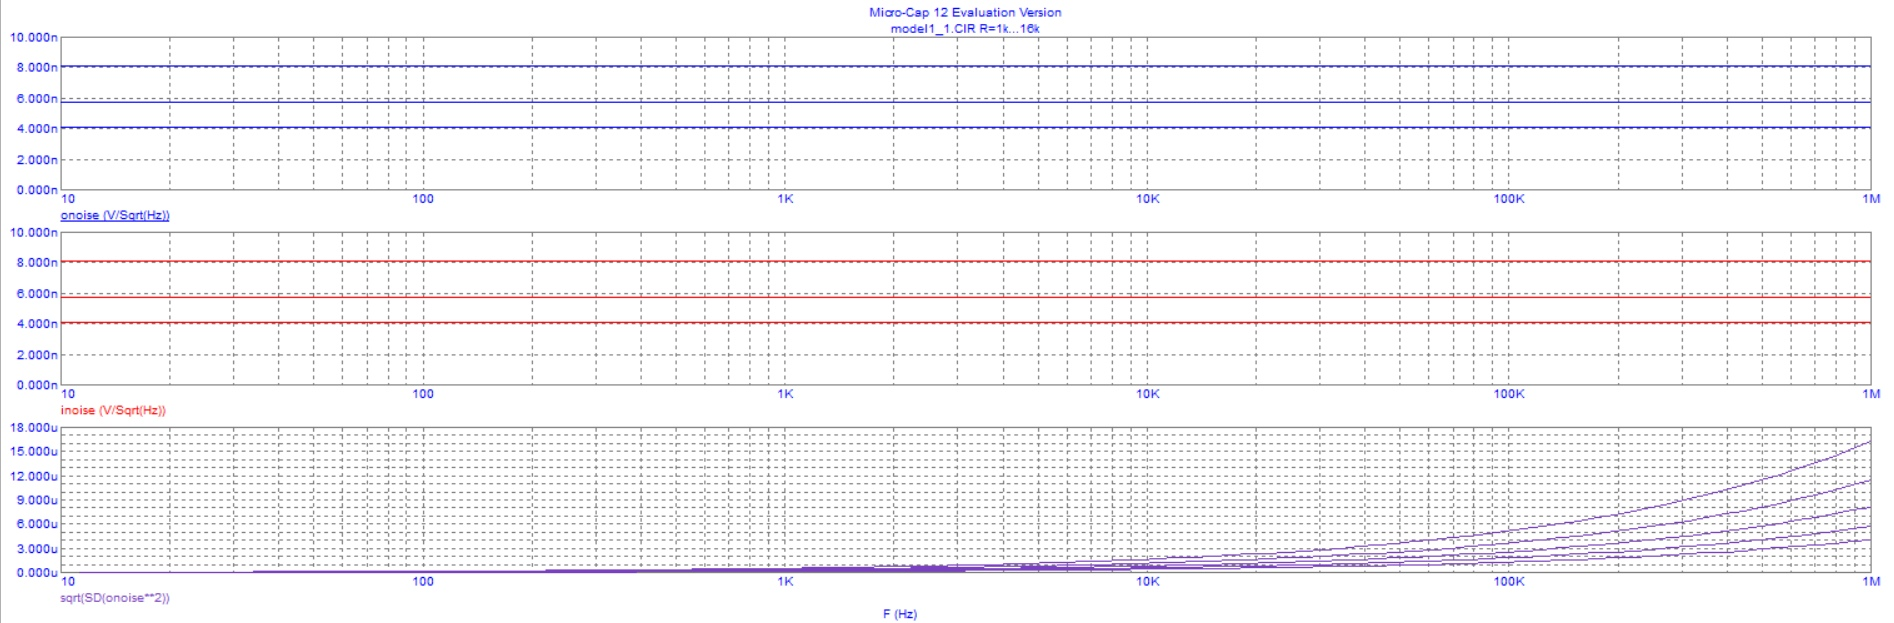
\includegraphics[width=1.1\linewidth]{pic1.jpg}
			\caption{Задание 1.1, пункт 2, Варьирование 1}
			\label{A}
\end{figure}

Первое варьирование: $R[1k, 16k | \log2]$

1) $R = 16k \Rightarrow \sigma = 16.138u$

2) $R = 8k \Rightarrow \sigma = 11.638u$

3) $R = 4k \Rightarrow \sigma = 8.224u$

4) $R = 2k \Rightarrow \sigma = 5.741u$

5) $R = 1k \Rightarrow \sigma = 4.198u$



\begin{figure}[h!]
	\centering
			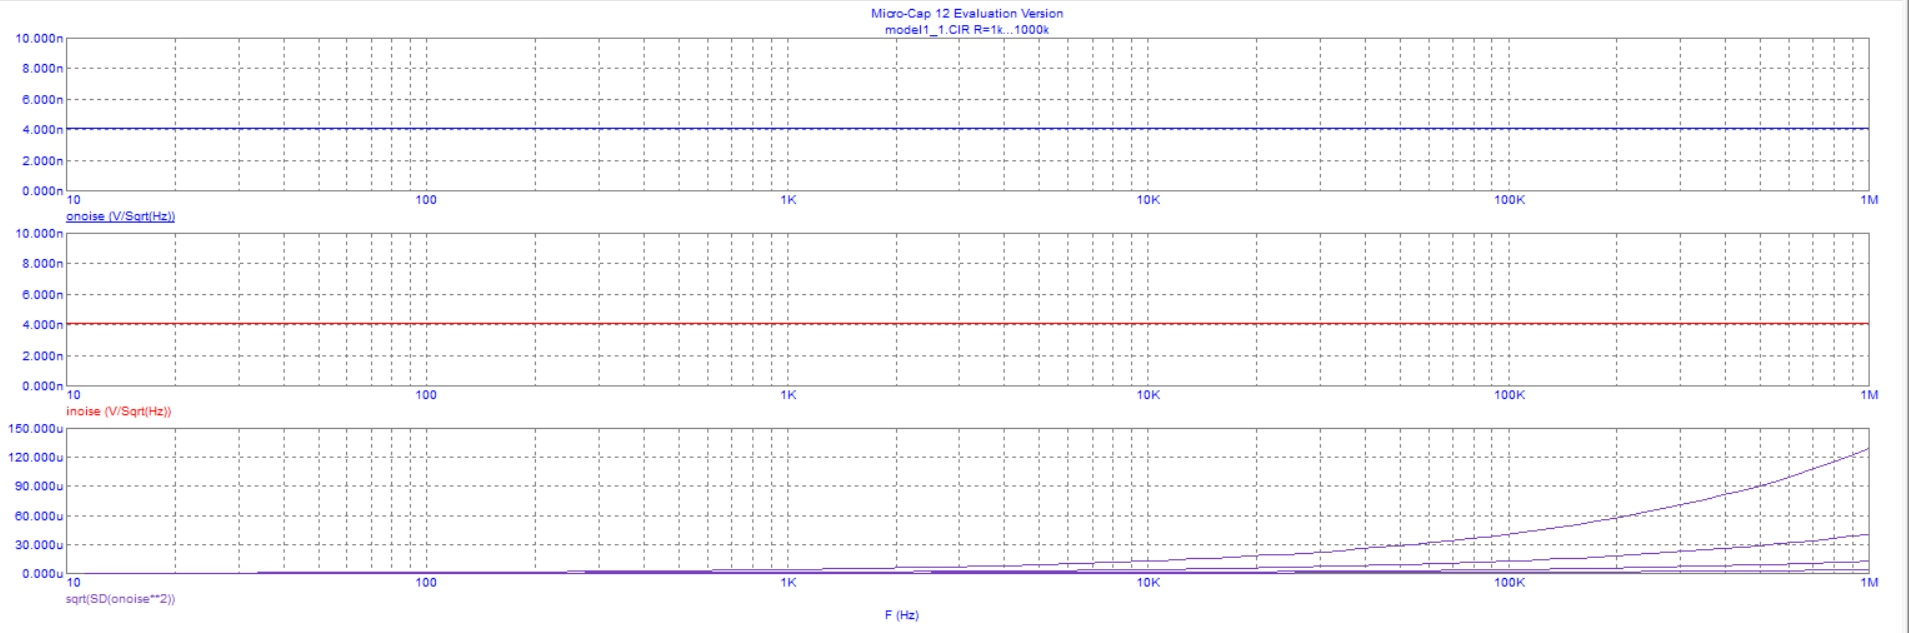
\includegraphics[width=1.1\linewidth]{pic2.jpg}
			\caption{Задание 1.1, пункт 2, Варьирование 2}
	\label{A}
\end{figure}

Второе варьирование: $R[1k, 1000k | \log10]$

1) $R = 1k \Rightarrow \sigma = 4.138u$

2) $R = 10k \Rightarrow \sigma = 12.931u$

3) $R = 100k \Rightarrow \sigma = 40.086u$

4) $R = 1000k \Rightarrow \sigma = 128.017u$


\textbf{3.}

Теперь перейдем к модели источника точка: $\{Is/ni\}$. Варьируя $R1[1k, 16k | Log2]$, проверим, что с увеличением $R1$ шумовое напряжение растет как $\sqrt{R}$, а ток падает как $\frac{1}{\sqrt{R}}$.

\begin{figure}[h!]
			\centering
			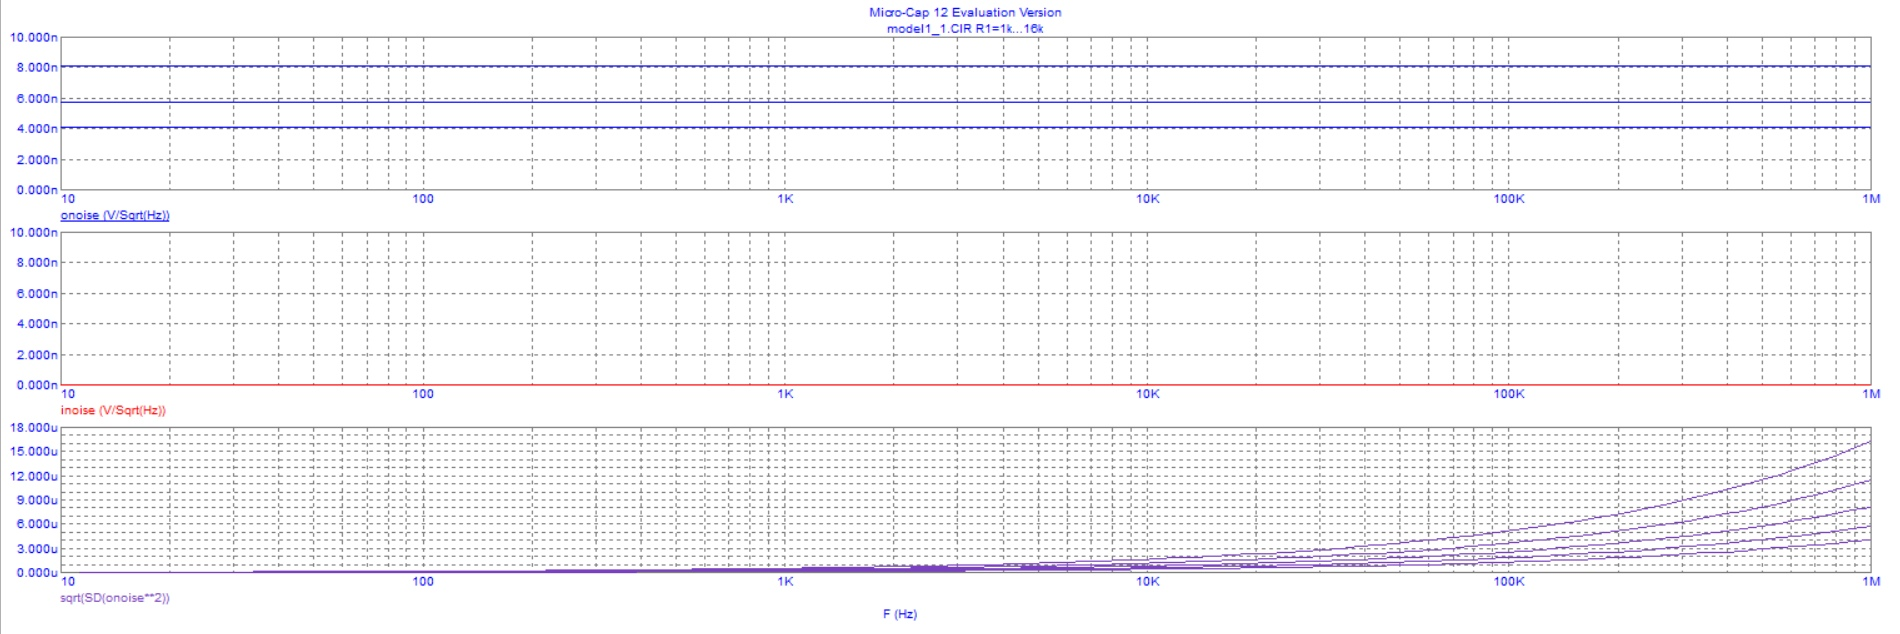
\includegraphics[width=1.1\linewidth]{pic3.jpg}
			\caption{Задание 1.1, пункт 3, Варьирование 1 для модели \{Is/ni\}}
			\label{A}
\end{figure}


Первое варьирование: $R[1k, 16k | \log2$]

1) $R = 1k \Rightarrow \sigma = 4.034u$

2) $R = 2k \Rightarrow \sigma = 5.741u$

3) $R = 4k \Rightarrow \sigma = 8.224u$

4) $R = 8k \Rightarrow \sigma = 11.328u$

5) $R = 16k \Rightarrow \sigma = 16.293u$


Замечаем, что напряжение растет как $\sqrt{R}$:

1) При $R_1 = 1k \Rightarrow  V_1 = 4.0n$

2) При $R_2 = 2k \Rightarrow  V_2 = 6.0n$

3) При $R_3 = 4k \Rightarrow  V_3 = 8.0n$

4) При $R_4 = 8k \Rightarrow  V_4 = 11.311n$

5) При $R_5 = 16k \Rightarrow  V_5 = 16.0n$

1) При $R_1 = 1k \Rightarrow  I_1 = 4.072p$

2) При $R_2 = 2k \Rightarrow  I_2 = 2.835p$

3) При $R_3 = 4k \Rightarrow  I_3 = 1.960p$

4) При $R_4 = 8k \Rightarrow  I_3 = 1,392p$

5) При $R_5 = 16k \Rightarrow  I_4 = 1.031p$


Замечаем, что напряжение растет как $\sqrt{R}$, т.к. $\frac{V_5}{V_4}$ $\approx 1,41 \approx \sqrt{\frac{16k}{8k}} \approx \sqrt{2} \approx 1.41$ и аналогично для других значений.

Заметим, что ток падает как $\frac{1}{\sqrt{R}}$.
Например, $\frac{I_2}{I_1} \approx 0.7$, при этом $\frac{R_1}{R_2} \approx \frac{1}{\sqrt{2}} \approx 0,72$. Аналогично проверяем для остальных значений.


\subsection{Сложение шумов}

$ $

$\textbf{1.}$

Рассмотрим модель с последовательным соединением $R_1, \: R_2$.

Проверим закон сложения шумовых напряжений.
\[ e(f) = \sqrt{4kT(R_1 + R_2)} \]

1) \textbf{Первое варьирование}: $R_1[0k, 1k | 1k]$, причем $R_2 = 2k$.

При $R_1 = 0k, \Rightarrow  e = 5.8n$.
Теоретическое значение $e \approx 5.75n$

При $R_1 = 1k, \Rightarrow  e = 7.00$
Теоретическое значение $e \approx 7.05n$

2) \textbf{Второе варьирование}: $R_2[0, 2k | 2k]$, причем $R_1 = 1k$.

При $R_2 = 0k, \Rightarrow  e = 4.00n$
Теоретическое значение $e \approx 4.07n$

При $R_2 = 2k, \Rightarrow  e = 7,05n$
Теоретическое значение $e \approx 7,00n$

Теоретические значения хорошо совпали с экспериментальными.

\begin{figure}[h!]
			\centering
			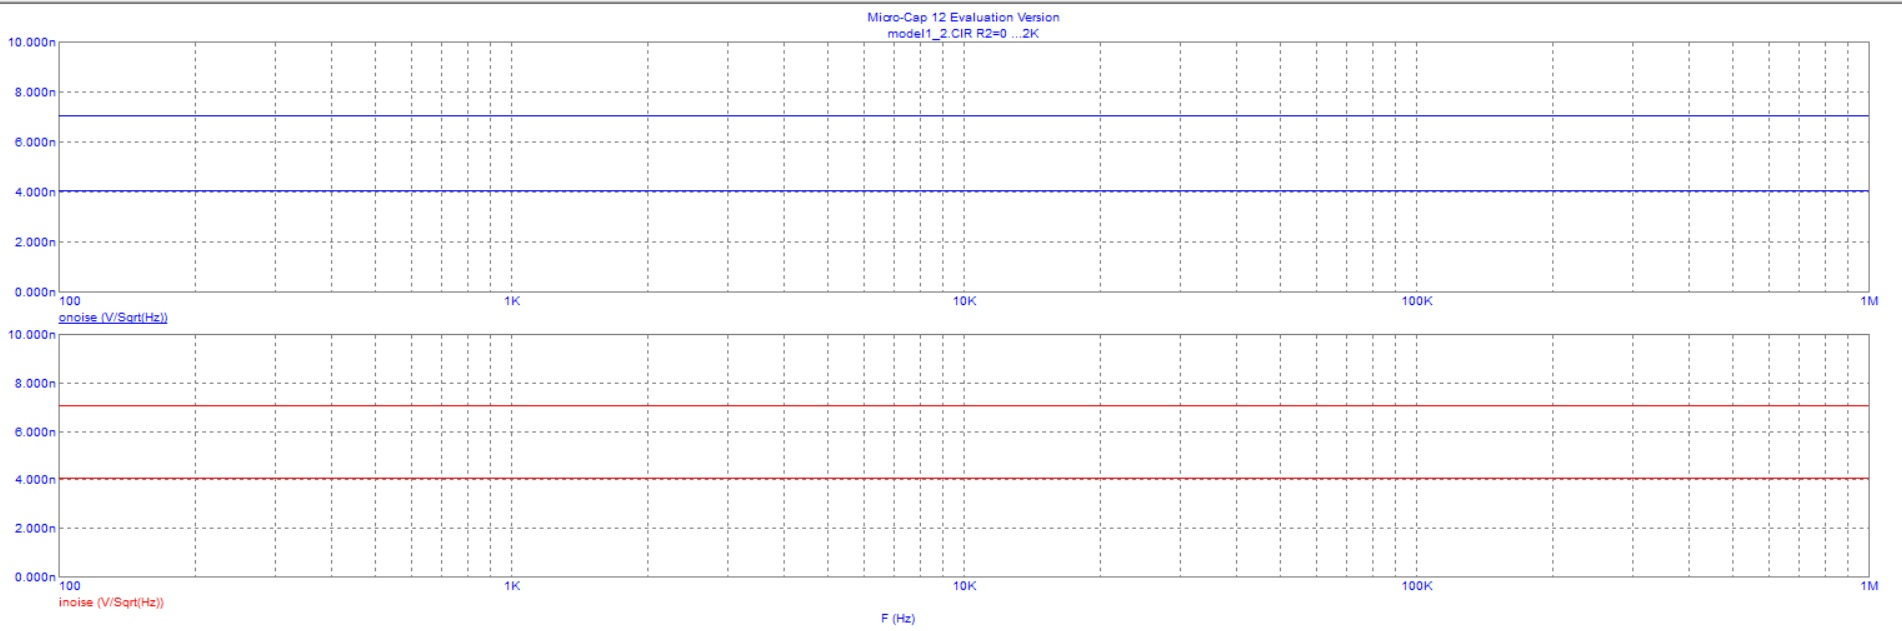
\includegraphics[width=1.1\linewidth]{1.2/pic4.jpg}
			\caption{Задание 1.2, пункт 1, Варьирование 1 для модели \{Es/se\}}
			\label{A}
\end{figure}

\begin{figure}[h!]
			\centering
			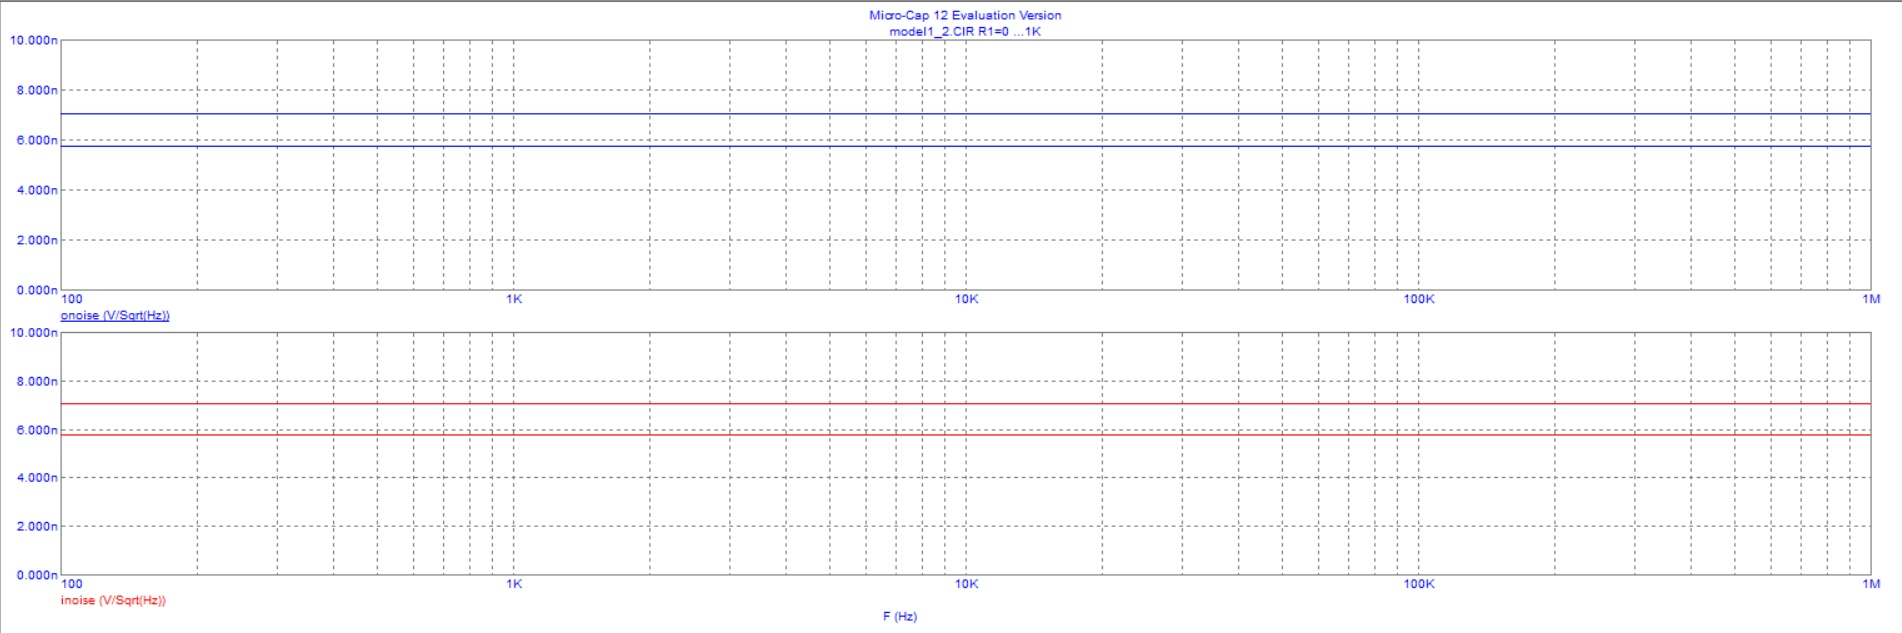
\includegraphics[width=1.1\linewidth]{1.2/pic5.jpg}
			\caption{Задание 1.2, пункт 1, Варьирование 2 для модели \{Es/se\}}
			\label{A}
\end{figure}



$\textbf{2.}$


Рассмотрим модель с параллельным соединением $R_3, \: R_4$ \{Is/ni\}

Проверим закон сложения шумовых токов:
\[ i(f) = \sqrt{\frac{4kT}{R_1 || R_2}}  \]

1) \textbf{Первое варьирование}: $R_3[1k, 100k | 99k]$, причем $R_4 = 2k$.

При $R_3 = 1k, \Rightarrow  i = 4,98p$.
Теоретическое значение $e \approx i = 5p$.

При $R_3 = 1k, \Rightarrow  i = 2.91p$.
Теоретическое значение $e \approx i = 2.94p$.

2) \textbf{Второе варьирование}: $R_4[2k, 100k | 98k]$, причем $R_3 = 1k$.

При $R_4 = 2k, \Rightarrow  i = 4.98p$.
Теоретическое значение $e \approx i = 5.00p$.

При $R_4 = 100k, \Rightarrow  i = 4.07p$.
Теоретическое значение $e \approx i = 4.09p$.

Теоретические значения хорошо совпали с экспериментальными.


\begin{figure}[h!]
			\centering
			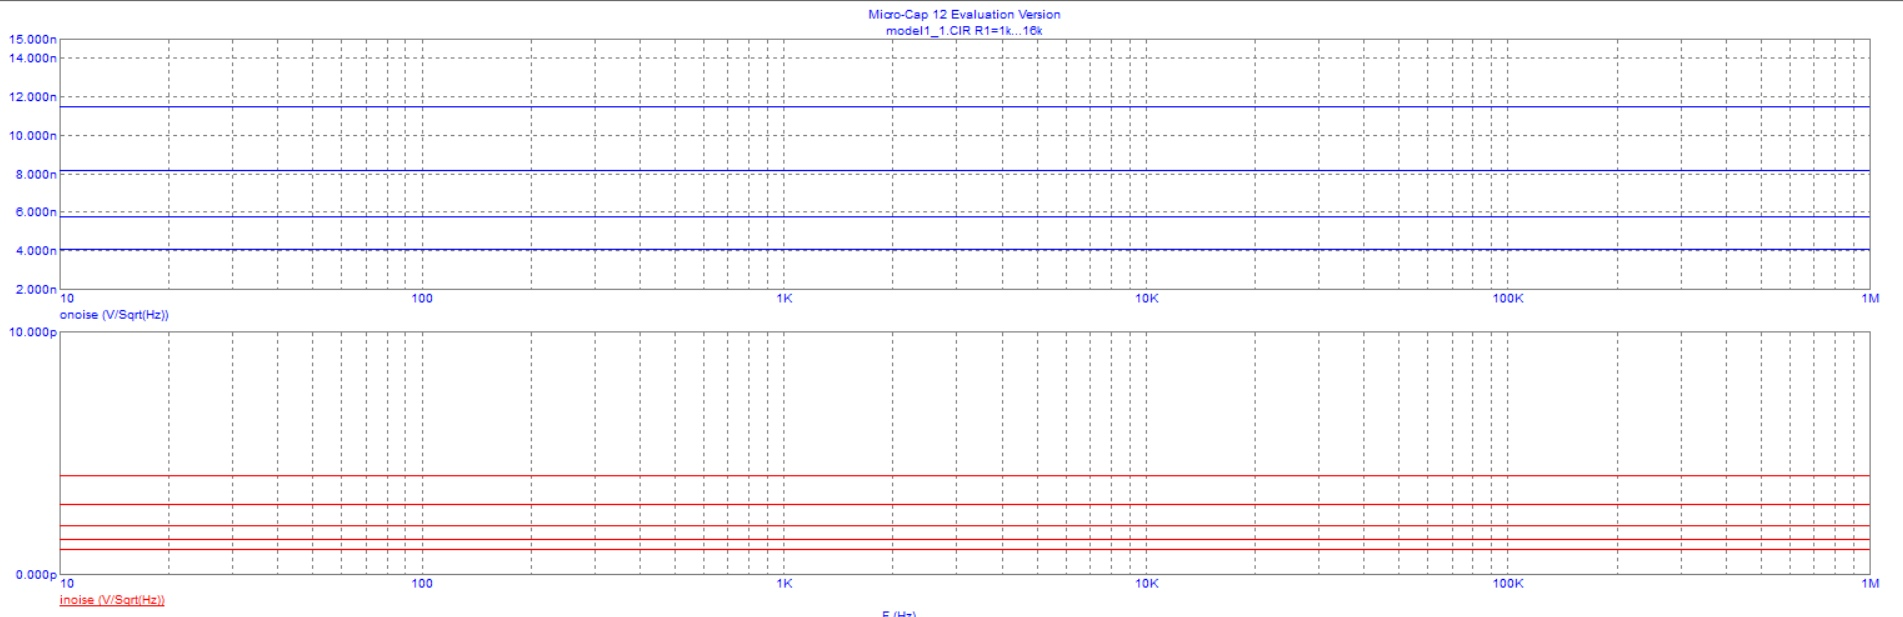
\includegraphics[width=1.1\linewidth]{1.2/pic6.jpg}
			\caption{Задание 1.2, пункт 2, Варьирование 1 для модели \{Is/ni\}}
			\label{A}
\end{figure}

\begin{figure}[h!]
			\centering
			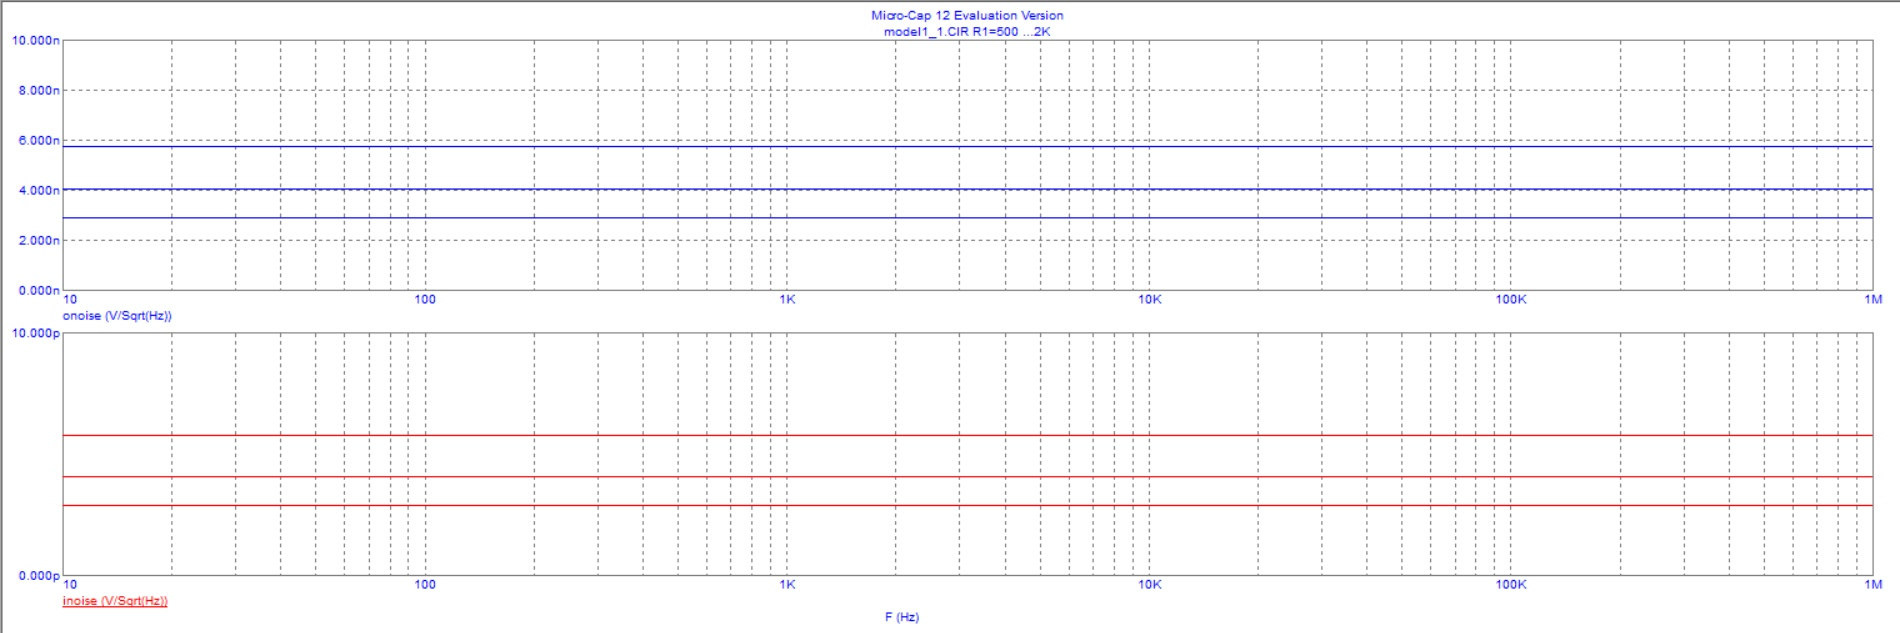
\includegraphics[width=1.1\linewidth]{1.2/pic7.jpg}
			\caption{Задание 1.2, пункт 2,Варьирование 2 для модели \{Is/ni\}}
			\label{A}
\end{figure}


\subsection{Шум в делителе напряжения}

$ $

$\textbf{1. }$


\begin{figure}[h!]
			\centering
			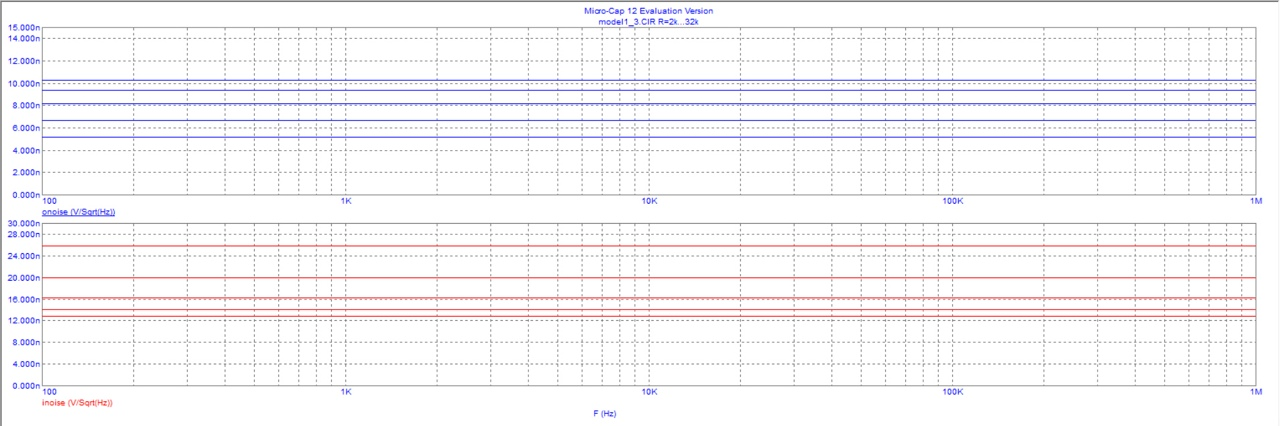
\includegraphics[width=1.1\linewidth]{1.3/pic8.jpg}
			\caption{Задание 1.3, пункт 1, данные для таблицы}
			\label{A}
\end{figure}

\begin{figure}[h!]
			\centering
			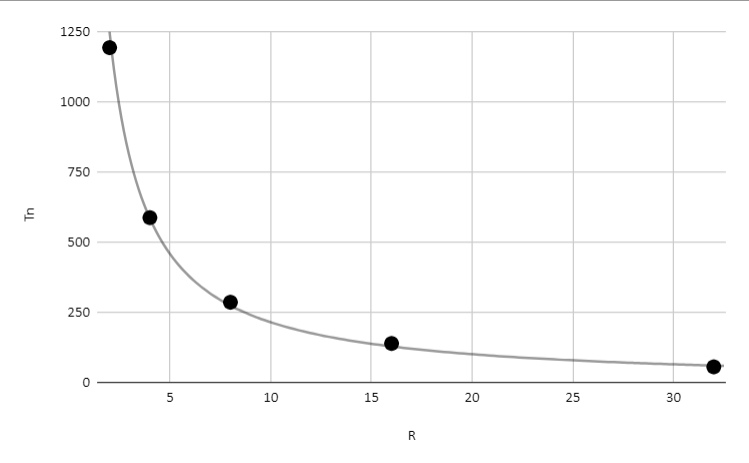
\includegraphics[width=1.1\linewidth]{1.3/pic9.jpg}
			\caption{Задание 1.3, пункт 1, График 1, $T_n(R)$}
			\label{A}
\end{figure}

\begin{figure}[h!]
			\centering
			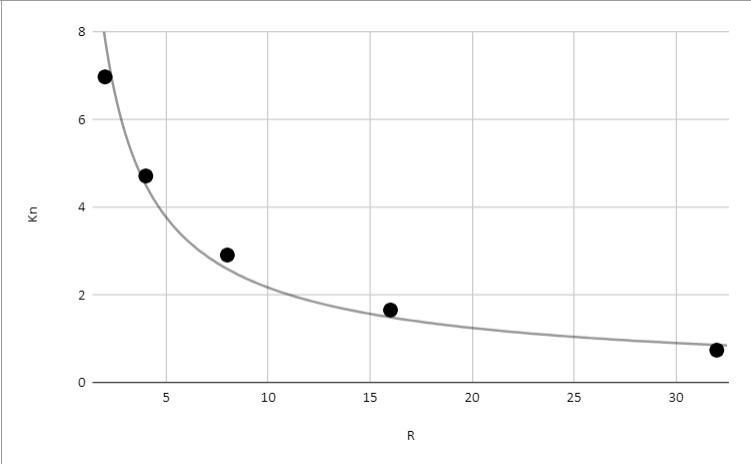
\includegraphics[width=1.1\linewidth]{1.3/pic10.jpg}
			\caption{Задание 1.3, пункт 1, График 2, $K_n(R)$}
			\label{A}
\end{figure}



\begin{table}[h!]
  \caption{Таблица для построения}
  \begin{center}
  	\begin{tabular}{|c|c|c|c|}
  	    \hline
  	$R_s, \: kOm$ & $e_n, \: nV$ & $K_n$ & $T_n, \: K$ \\
  	    \hline
  	8 & 25.680 &  & 1193.34   \\
  		\hline
  	8 & 19.794 &  & 587.23    \\
  		\hline
  	8 & 16.082  &   & 285.66   \\
  		\hline
    8 & 13.918  &   &  138.65   \\
        \hline
    8 & 12.526  &   & 55.30    \\
        \hline
  	\end{tabular}
  \end{center}
\label{B_table}
\end{table}


\newpage
\newpage

\section{Дробовой шум}

$ $

$\textbf{1.}$

\begin{figure}[h!]
			\centering
			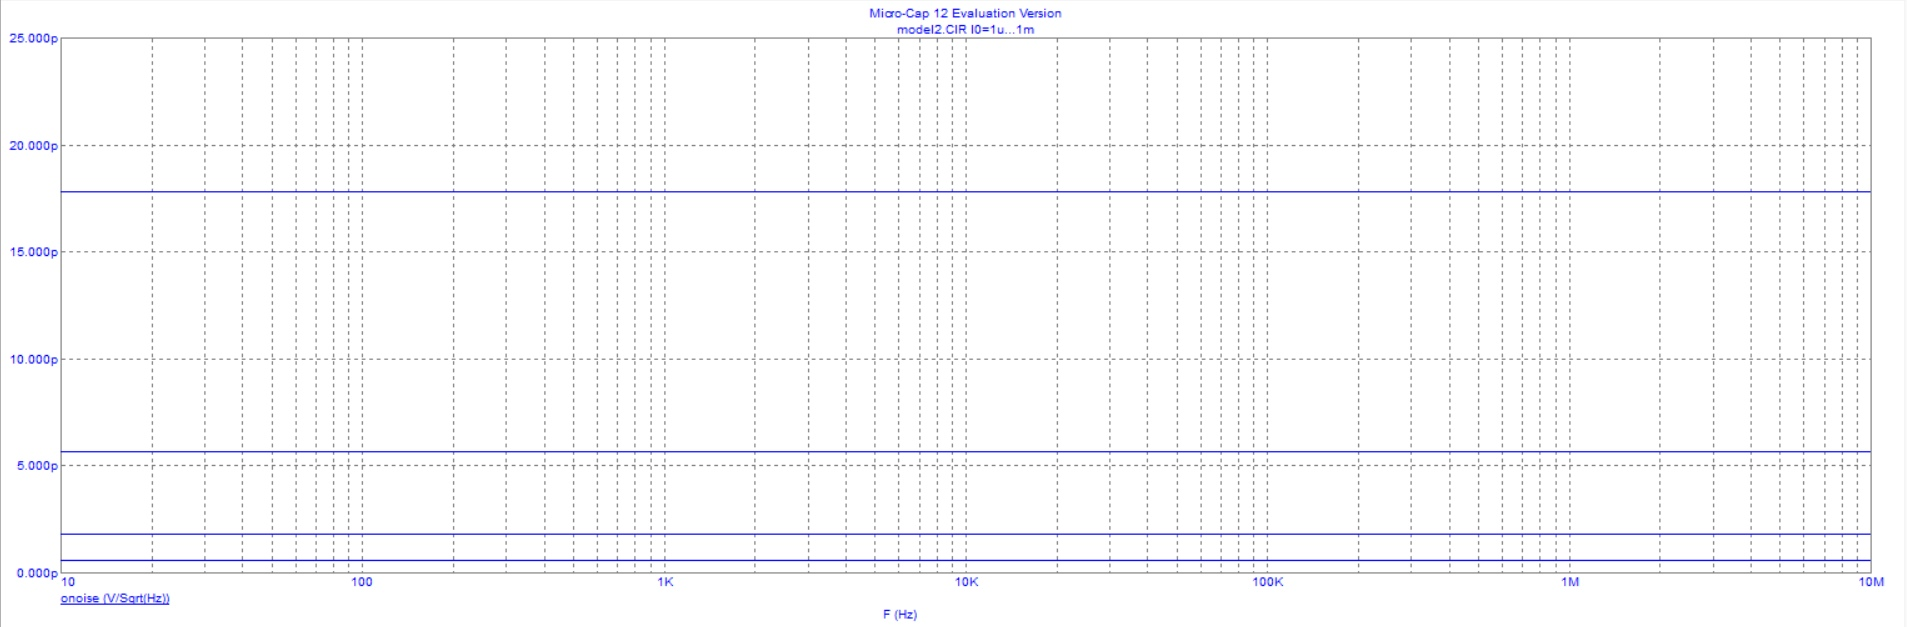
\includegraphics[width=1.1\linewidth]{2.1/pic12.jpg}
			\caption{Задание 2.1, пункт 1}
			\label{A}
\end{figure}


1)$I_{01} = 1m \Rightarrow e_1 = 17.8p$

2)$I_{02} = 100u \Rightarrow e_2 = 5.7p$

3)$I_{03} = 10u \Rightarrow e_3 = 1.8p$

4)$I_{04} = 1u \Rightarrow e_4 = 0.5p$


Проверим, что $\frac{e_1}{e_2} = \frac{\sqrt{I_{02}}}{\sqrt{I_{01}}}$


\begin{figure}[h!]
			\centering
			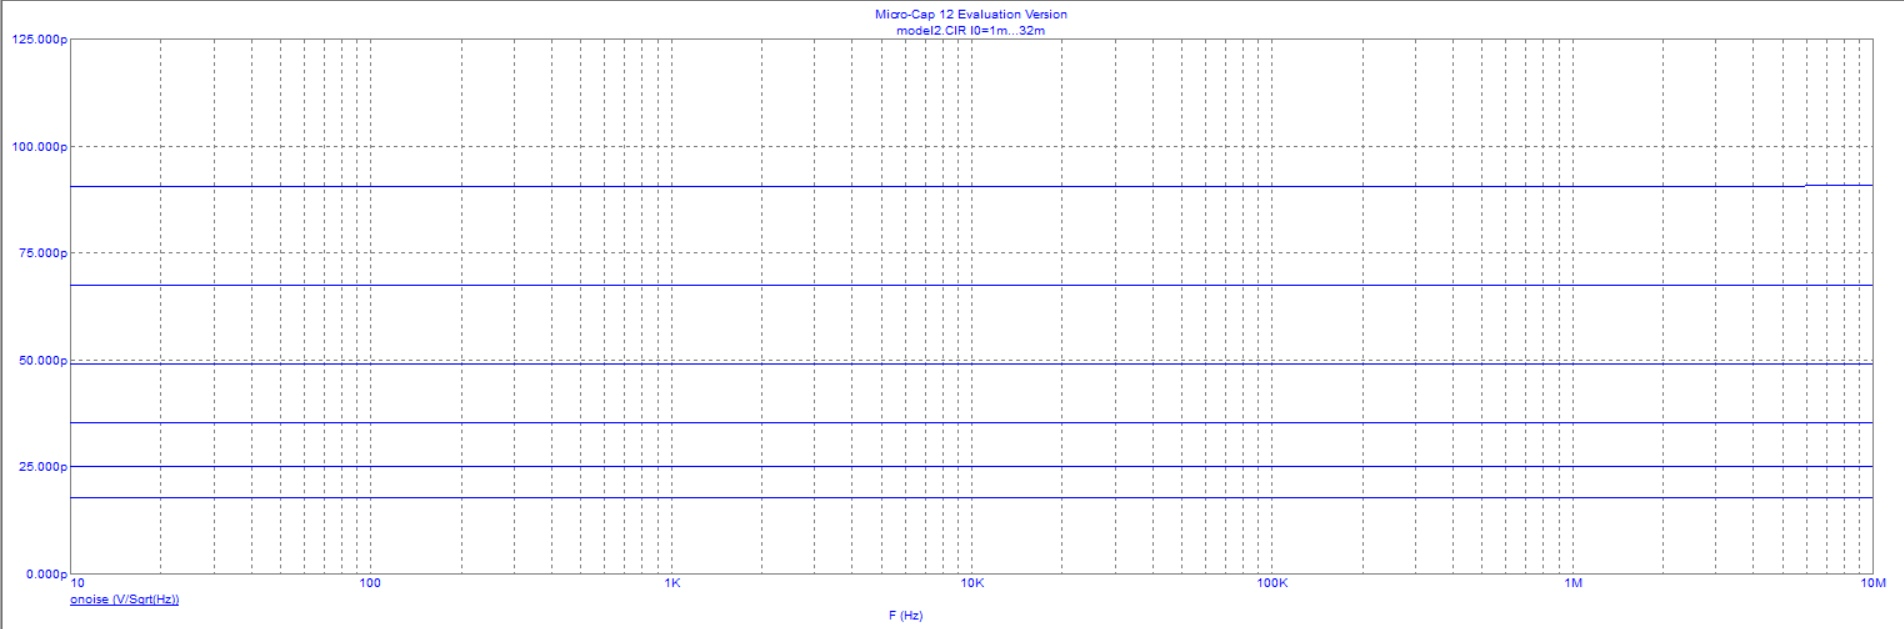
\includegraphics[width=1.1\linewidth]{2.1/pic11.jpg}
			\caption{Задание 2.1, пункт 2}
			\label{A}
\end{figure}


1) $I_{01} = 32m \Rightarrow e_1 = 98.5p$

2) $I_{02} = 16m \Rightarrow e_2 = 67.5p$

3) $I_{03} = 8m \Rightarrow  e_3 = 48.8p$

4) $I_{04} = 4m \Rightarrow e_4 = 35.0p$

5) $I_{05} = 2m \Rightarrow e_4 = 24.8p$

6) $I_{06} = 1m \Rightarrow e_4 = 17.5p$


Проверим, что $\frac{e_1}{e_2} = \frac{\sqrt{I_{02}}}{\sqrt{I_{01}}}$

$\textbf{2.}$

Учтем, что $r_D \approx K\cdot R_1$, причем $R_1 = 10K$

1)$I_{01} = 1u, K = 838.2m \Rightarrow r_{D_{01}} = 8.38K$

2)$I_{02} = 10u, K = 338.8m \Rightarrow r_{D_{02}} = 3.38K$

3)$I_{03} = 100u, K = 46.7m  \Rightarrow r_{D_{03}} = 460$

4)$I_{04} = 1m, K = 2.9m \Rightarrow r_{D_{04}} = 29$


\begin{figure}[h!]
			\centering
			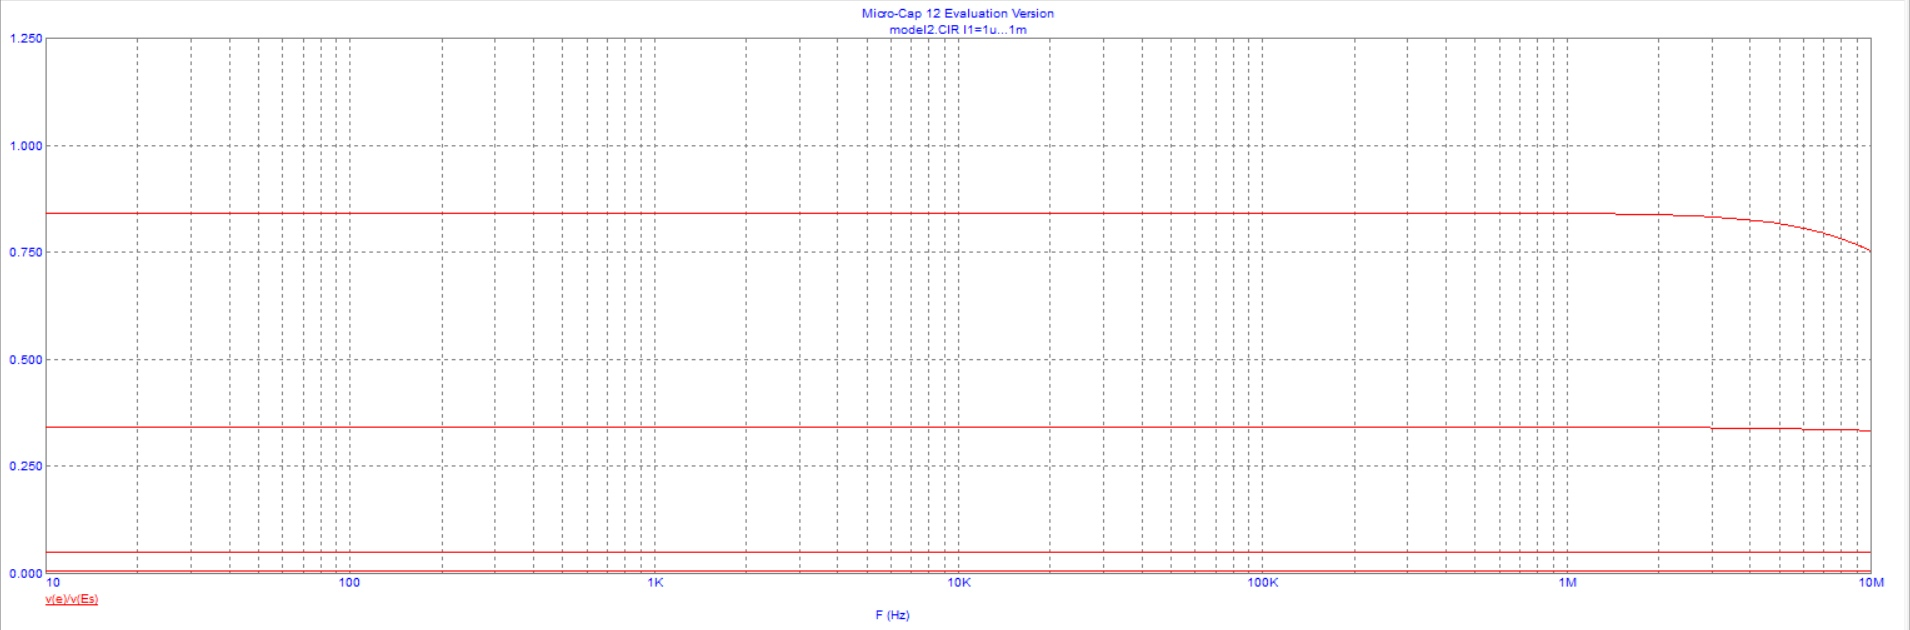
\includegraphics[width=1.1\linewidth]{2.1/pic13.jpg}
			\caption{Задание 2.1, пункт 2}
			\label{A}
\end{figure}


$\textbf{3.}$

1) $I_1 = 1u, \Rightarrow e = 14.6n$

2) $I_1 = 10u, \Rightarrow e = 4.6n $

3) $I_1 = 100u , \Rightarrow  e = 1.4n $

4) $I_1 = 1m , \Rightarrow e = 420.6p$

5) $I_1 = 10m,  \Rightarrow e = 93.5p$

Проверяем формулу $e(f) = i(f)\cdot r_d$, при варьированиее $I_1[1u, 10m | Log10] $.

Причем $i(f) = \sqrt{2qI_0}$.

1) $i_1(f) = 5.65\cdot 10^{-13} \Rightarrow e = R_{D_{01}} \cdot i_1(f)  = 4.7n$

1) $i_1(f) = 1.78\cdot 10^{-12} \Rightarrow e = R_{D_{02}} \cdot i_1(f) = 6n$





\newpage

\section{Фильтрация шумов}

\subsection{Установить $\frac{V1}{n1}$ (интегрирующая цепь)}

$ $

$\textbf{1.}$



Открываем файл model3.
Устанавливаем интегрирующую цепь.
По графику рис.14 определяем граничную частоту $f_h$.
Получаем $f_h = 10148 Hz$.


\begin{figure}[h!]
			\centering
			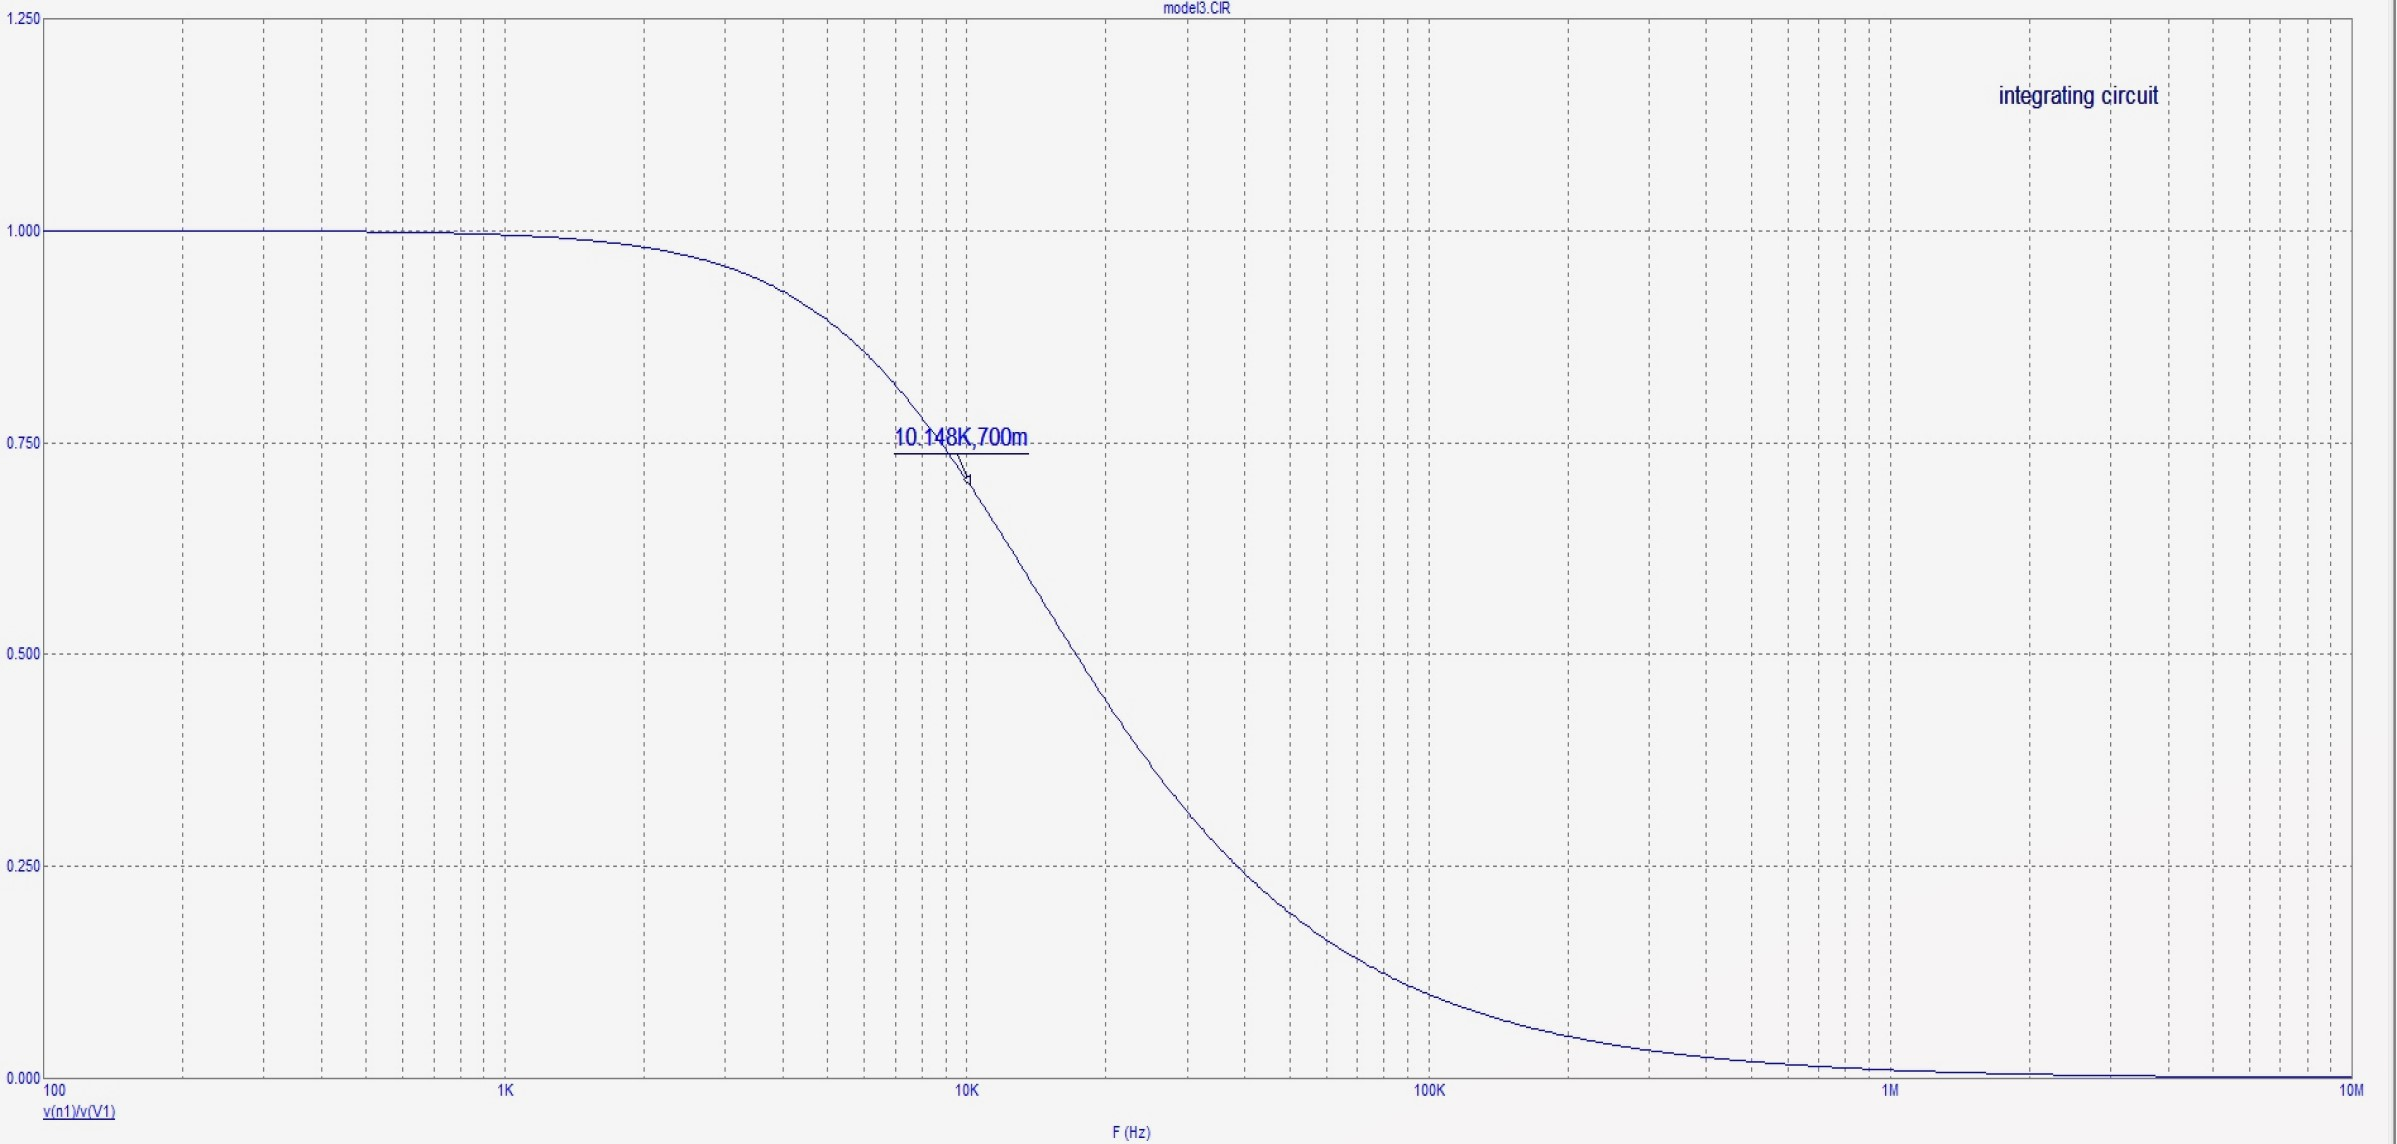
\includegraphics[width=1.1\linewidth]{3/3_1_1.jpg}
			\caption{Задание 3.1, пункт 1}
			\label{A}
\end{figure}

$\textbf{2.} $


Переключимся на шумовые графики. Измерим шумовое напряжение $n_1$ в полосе пропускания, уровень шума на выходе $\sigma$.

Проверим, что $\sigma = n_1\cdot \sqrt{F_n} = \sqrt{\frac{kT}{C}}$, причем $F_n = \frac{\pi}{2} \cdot f_n$.

Измерения, вычисления так же приведены на скриншоте.

$n_1 = 12.874n$

$\sigma_{pract} = 1.604$, $\sigma_{theor} = 1.627$.


\begin{figure}[h!]
			\centering
			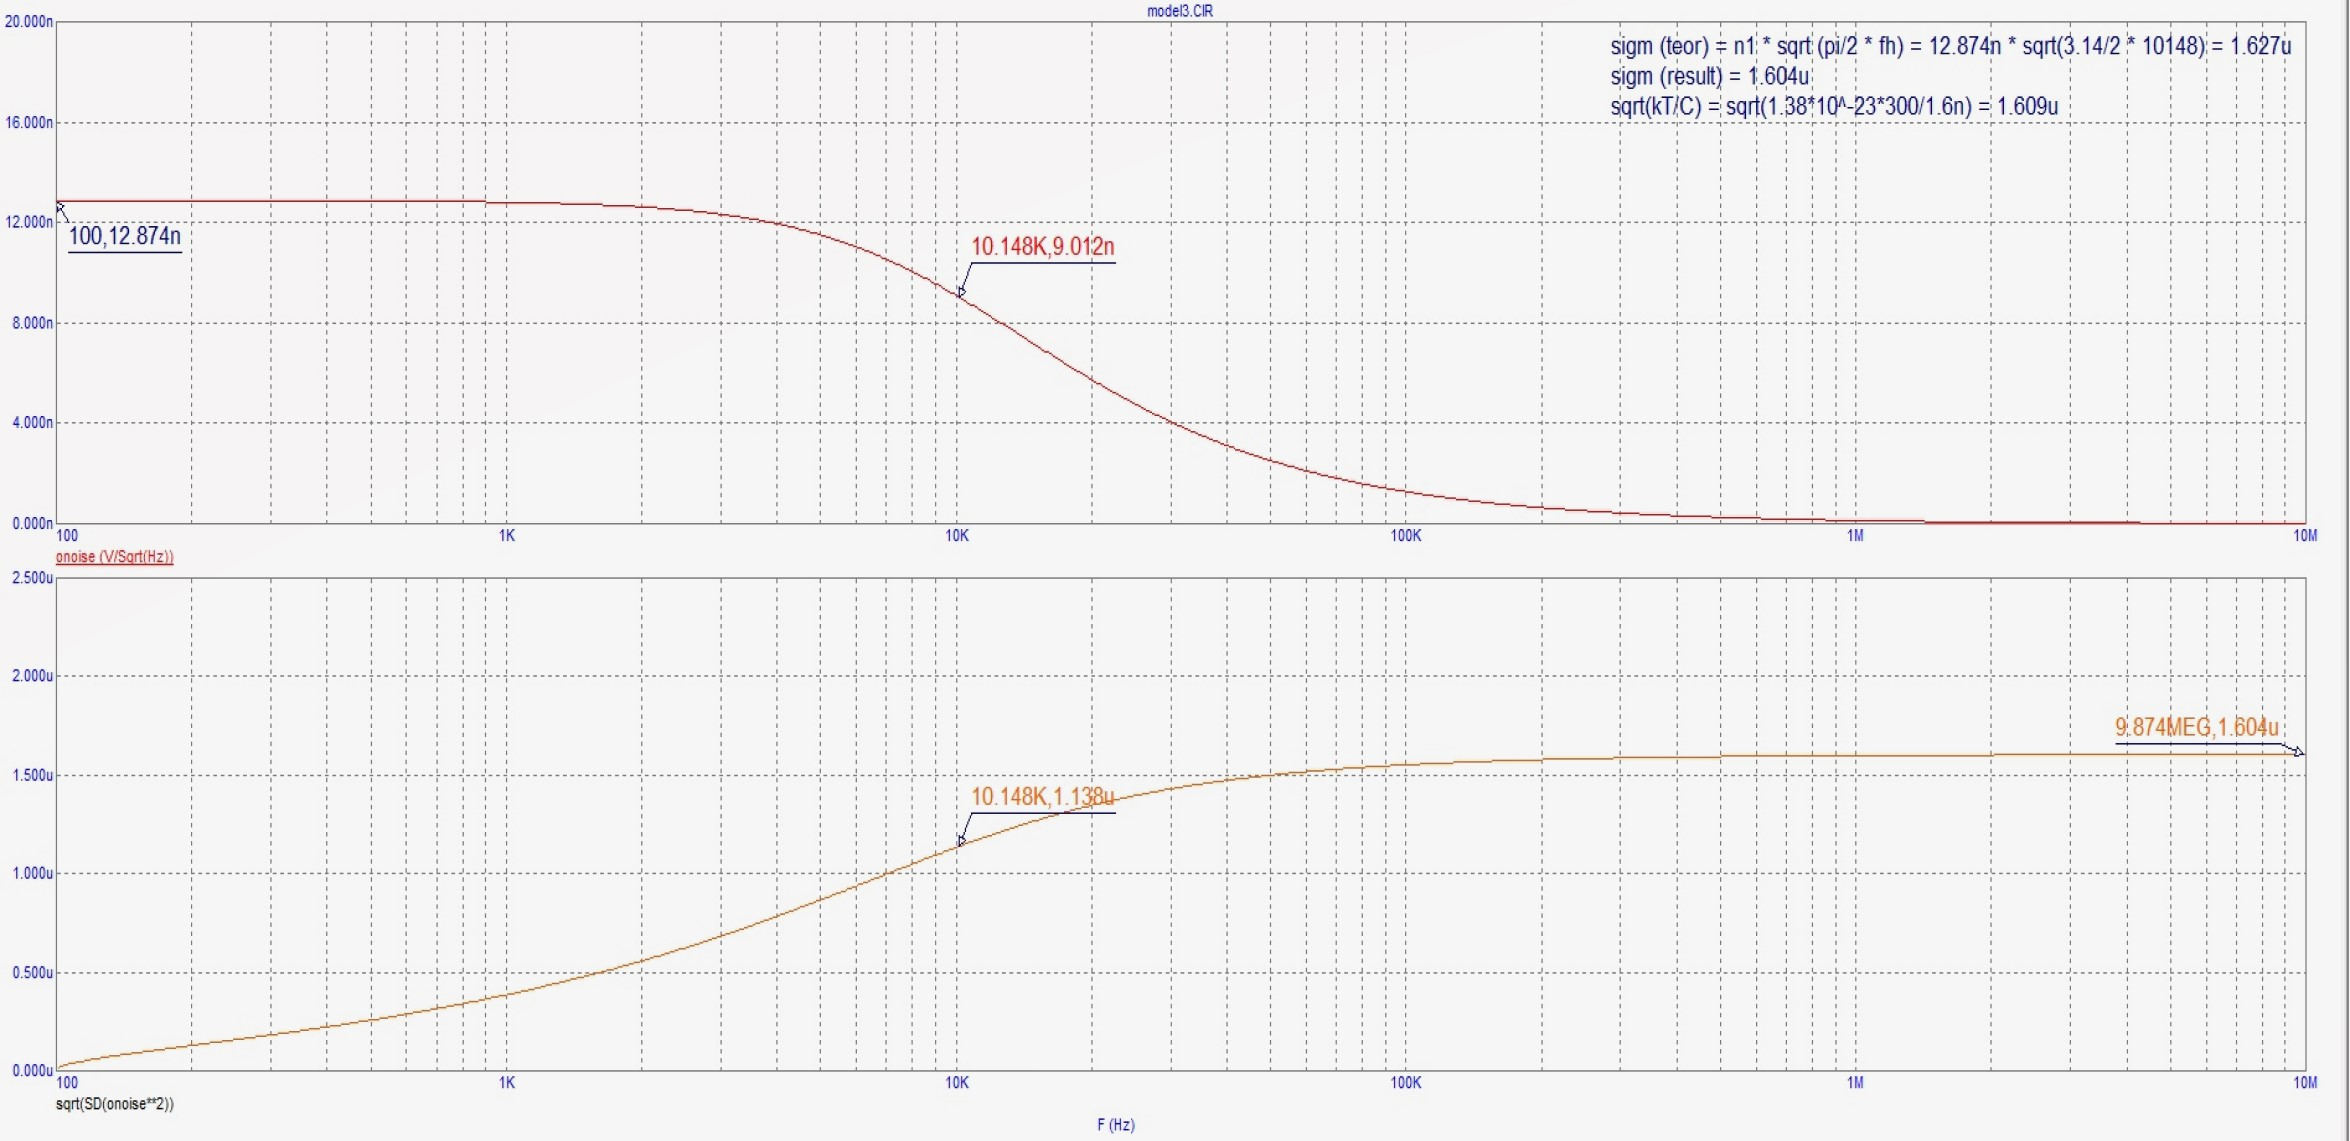
\includegraphics[width=1.1\linewidth]{3/3_1_2.jpg}
			\caption{Задание 3.1, пункт 2}
			\label{A}
\end{figure}


$\textbf{3.}$


Варьирование $R_1[2k, 16k | 4k]$.
Снимаем зависимость шумового напряжения от $R_1$.

\begin{figure}[h!]
			\centering
			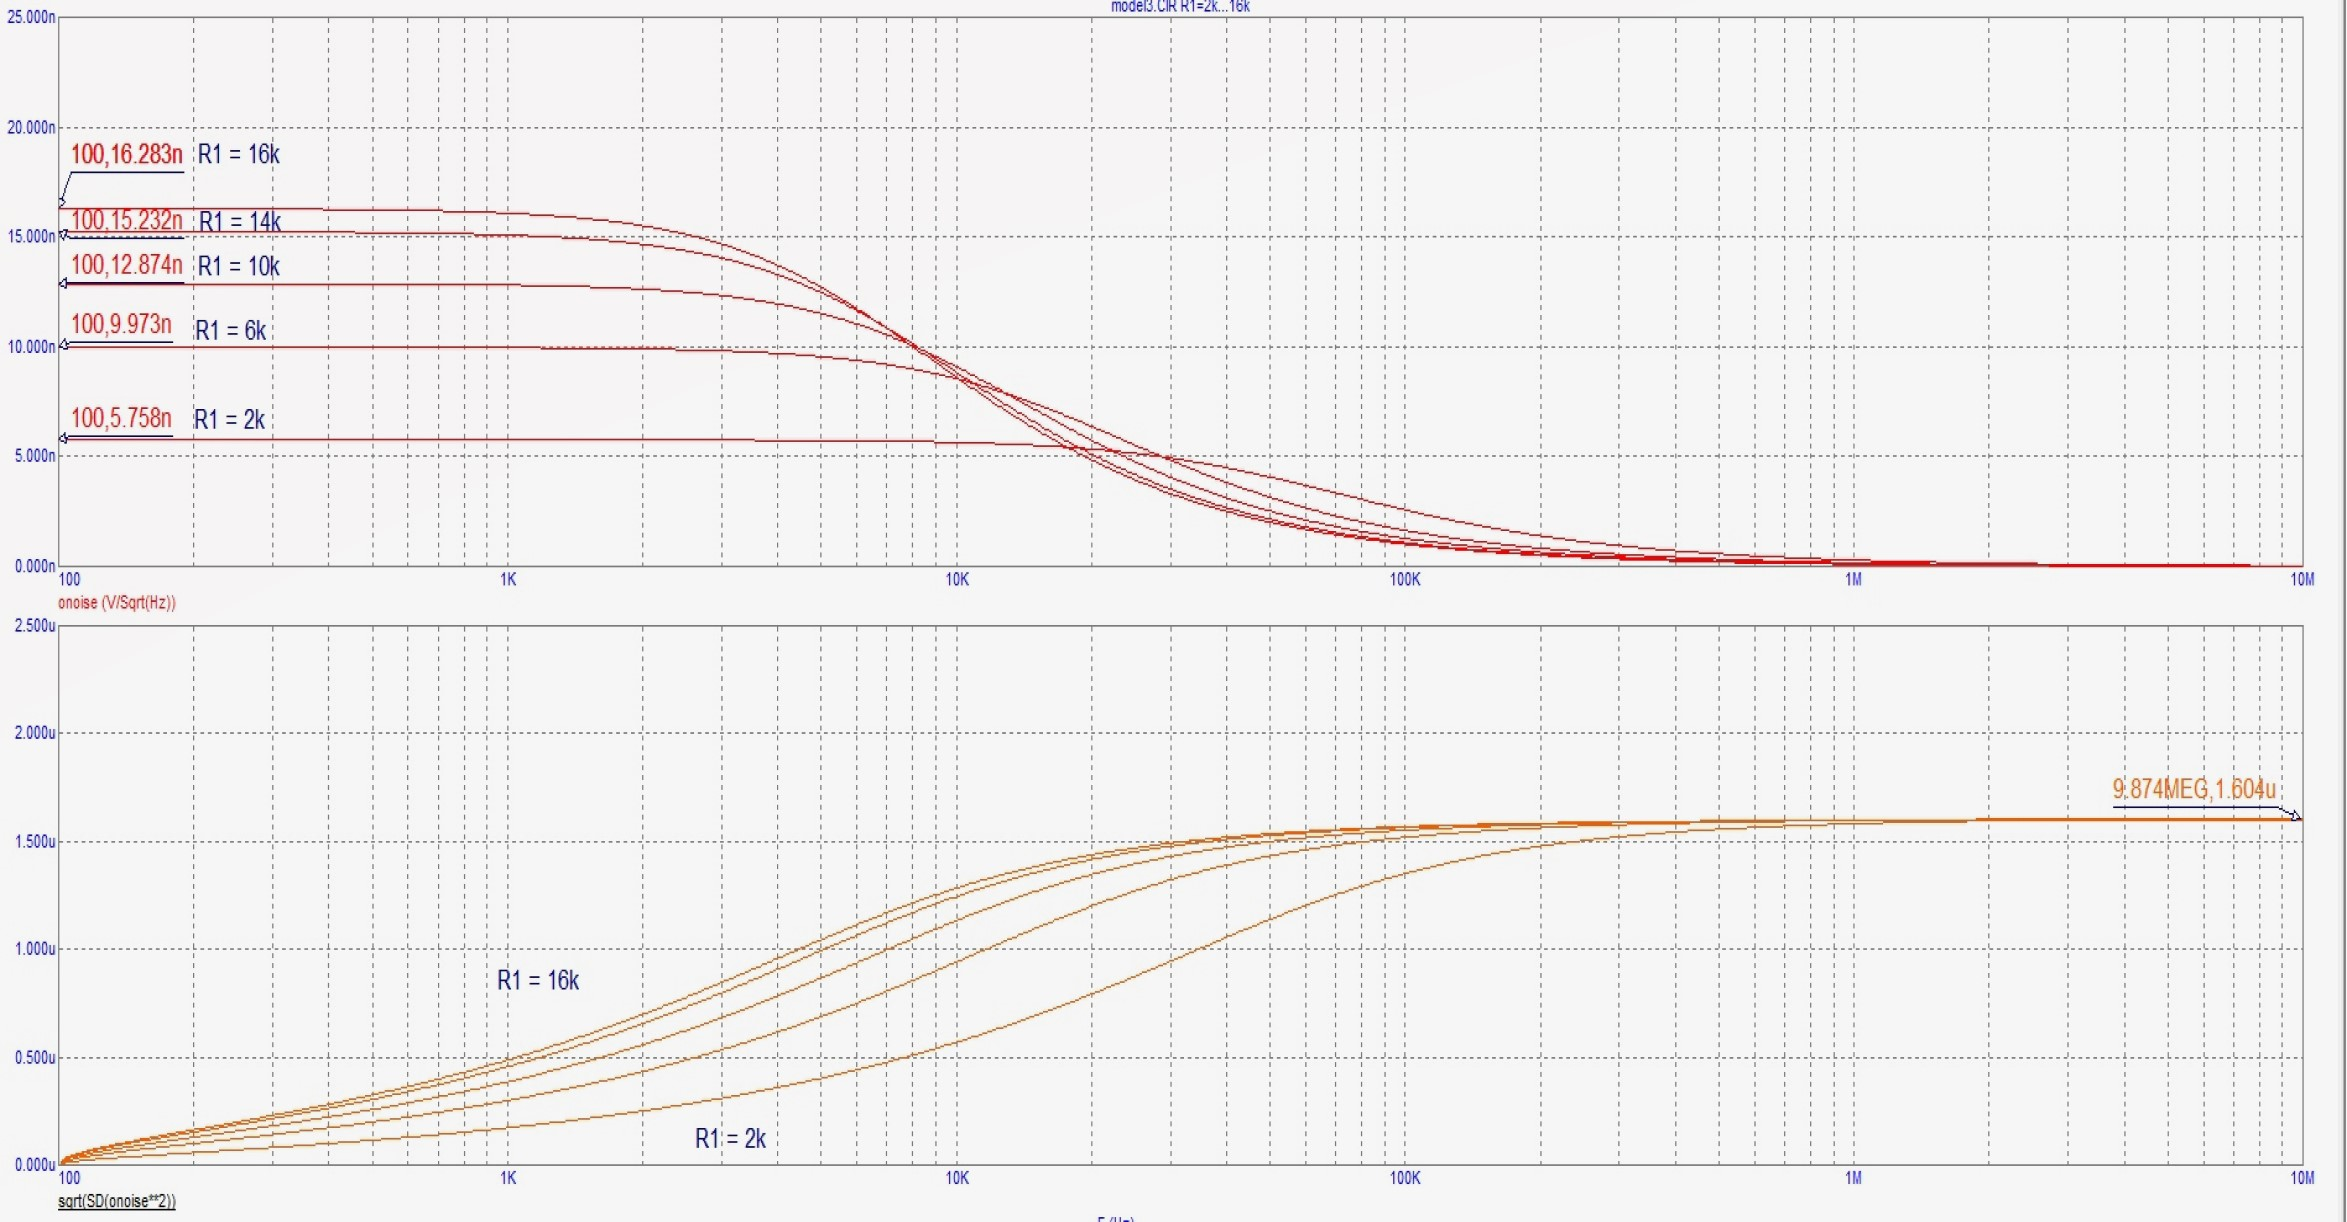
\includegraphics[width=1.1\linewidth]{3/3_1_4.jpg}
			\caption{Задание 3.1, пункт 3}
			\label{A}
\end{figure}


$\textbf{4.}$


Варьирование $C_1[0.8n, 2.4n | 0.4k]$.
Cнимаем зависимость уровня шума от емкости.

\begin{figure}[h!]
			\centering
			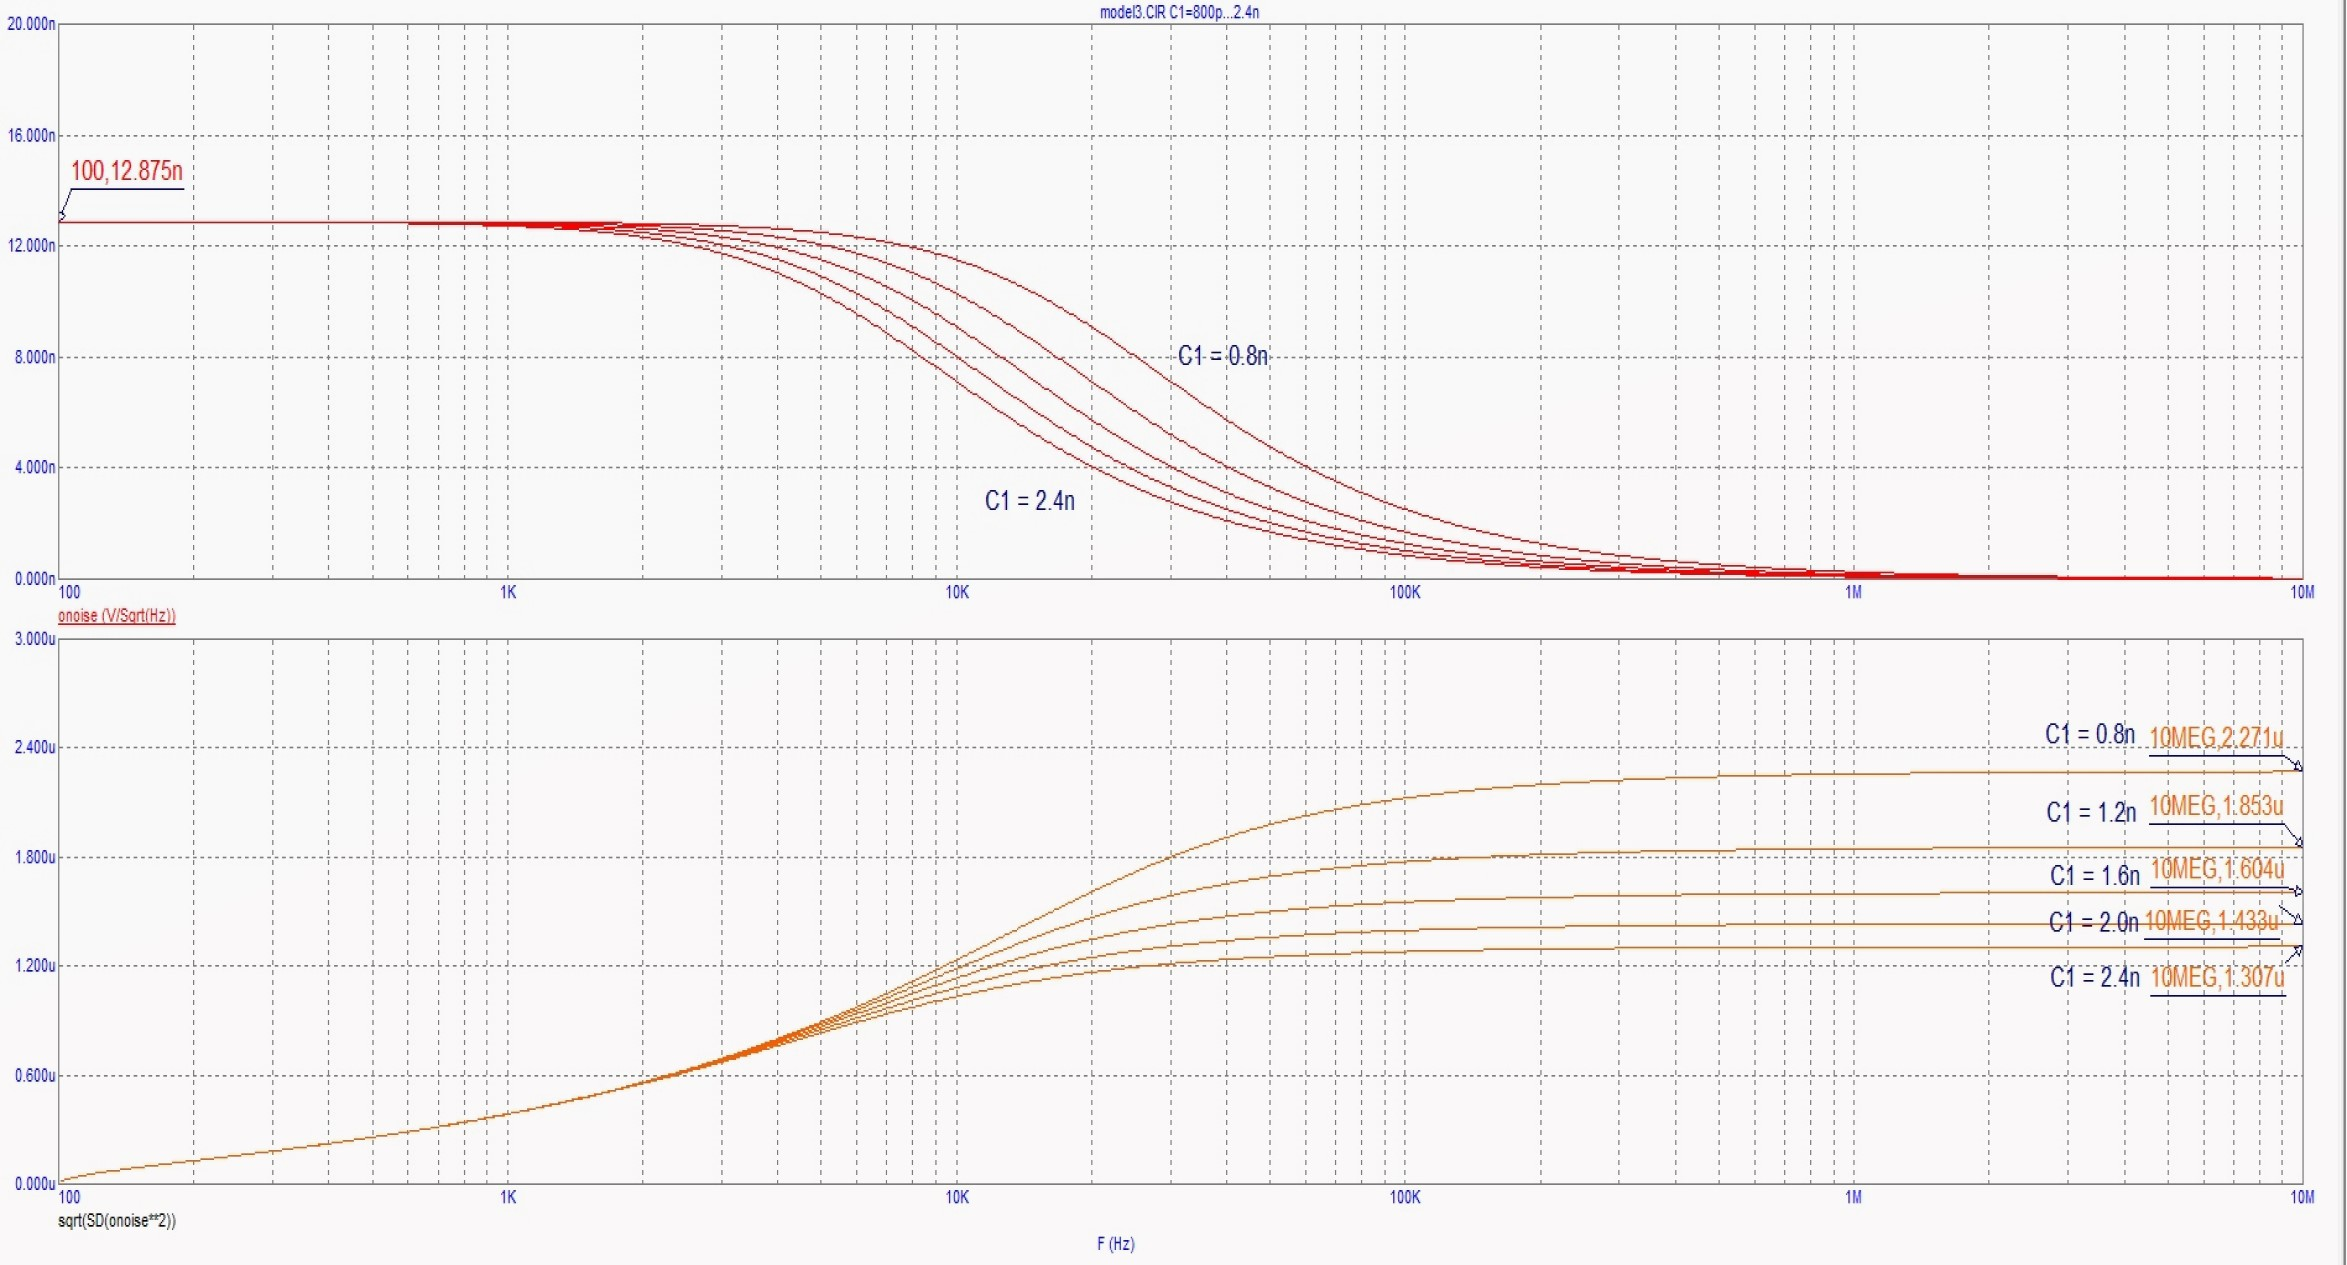
\includegraphics[width=1.1\linewidth]{3/3_1_3.jpg}
			\caption{Задание 3.1, пункт 4}
			\label{A}
\end{figure}

\subsection{Установить $\frac{V2}{n2}$ (полосовой $LC$--фильтр)}

Теперь рассматрим полосовой LC-фильтр.

$\textbf{1.}$


По графику оцениваем резонансную частоту и полосу пропускания по уровню 0,7. Оцениваем добротность. Получаем:

$f_0 = 100694 \: Hz$, $\Delta f = 20626 \: Hz$, $Q = \frac{f_0}{\Delta f} \approx 4.8$.

\begin{figure}[h!]
			\centering
			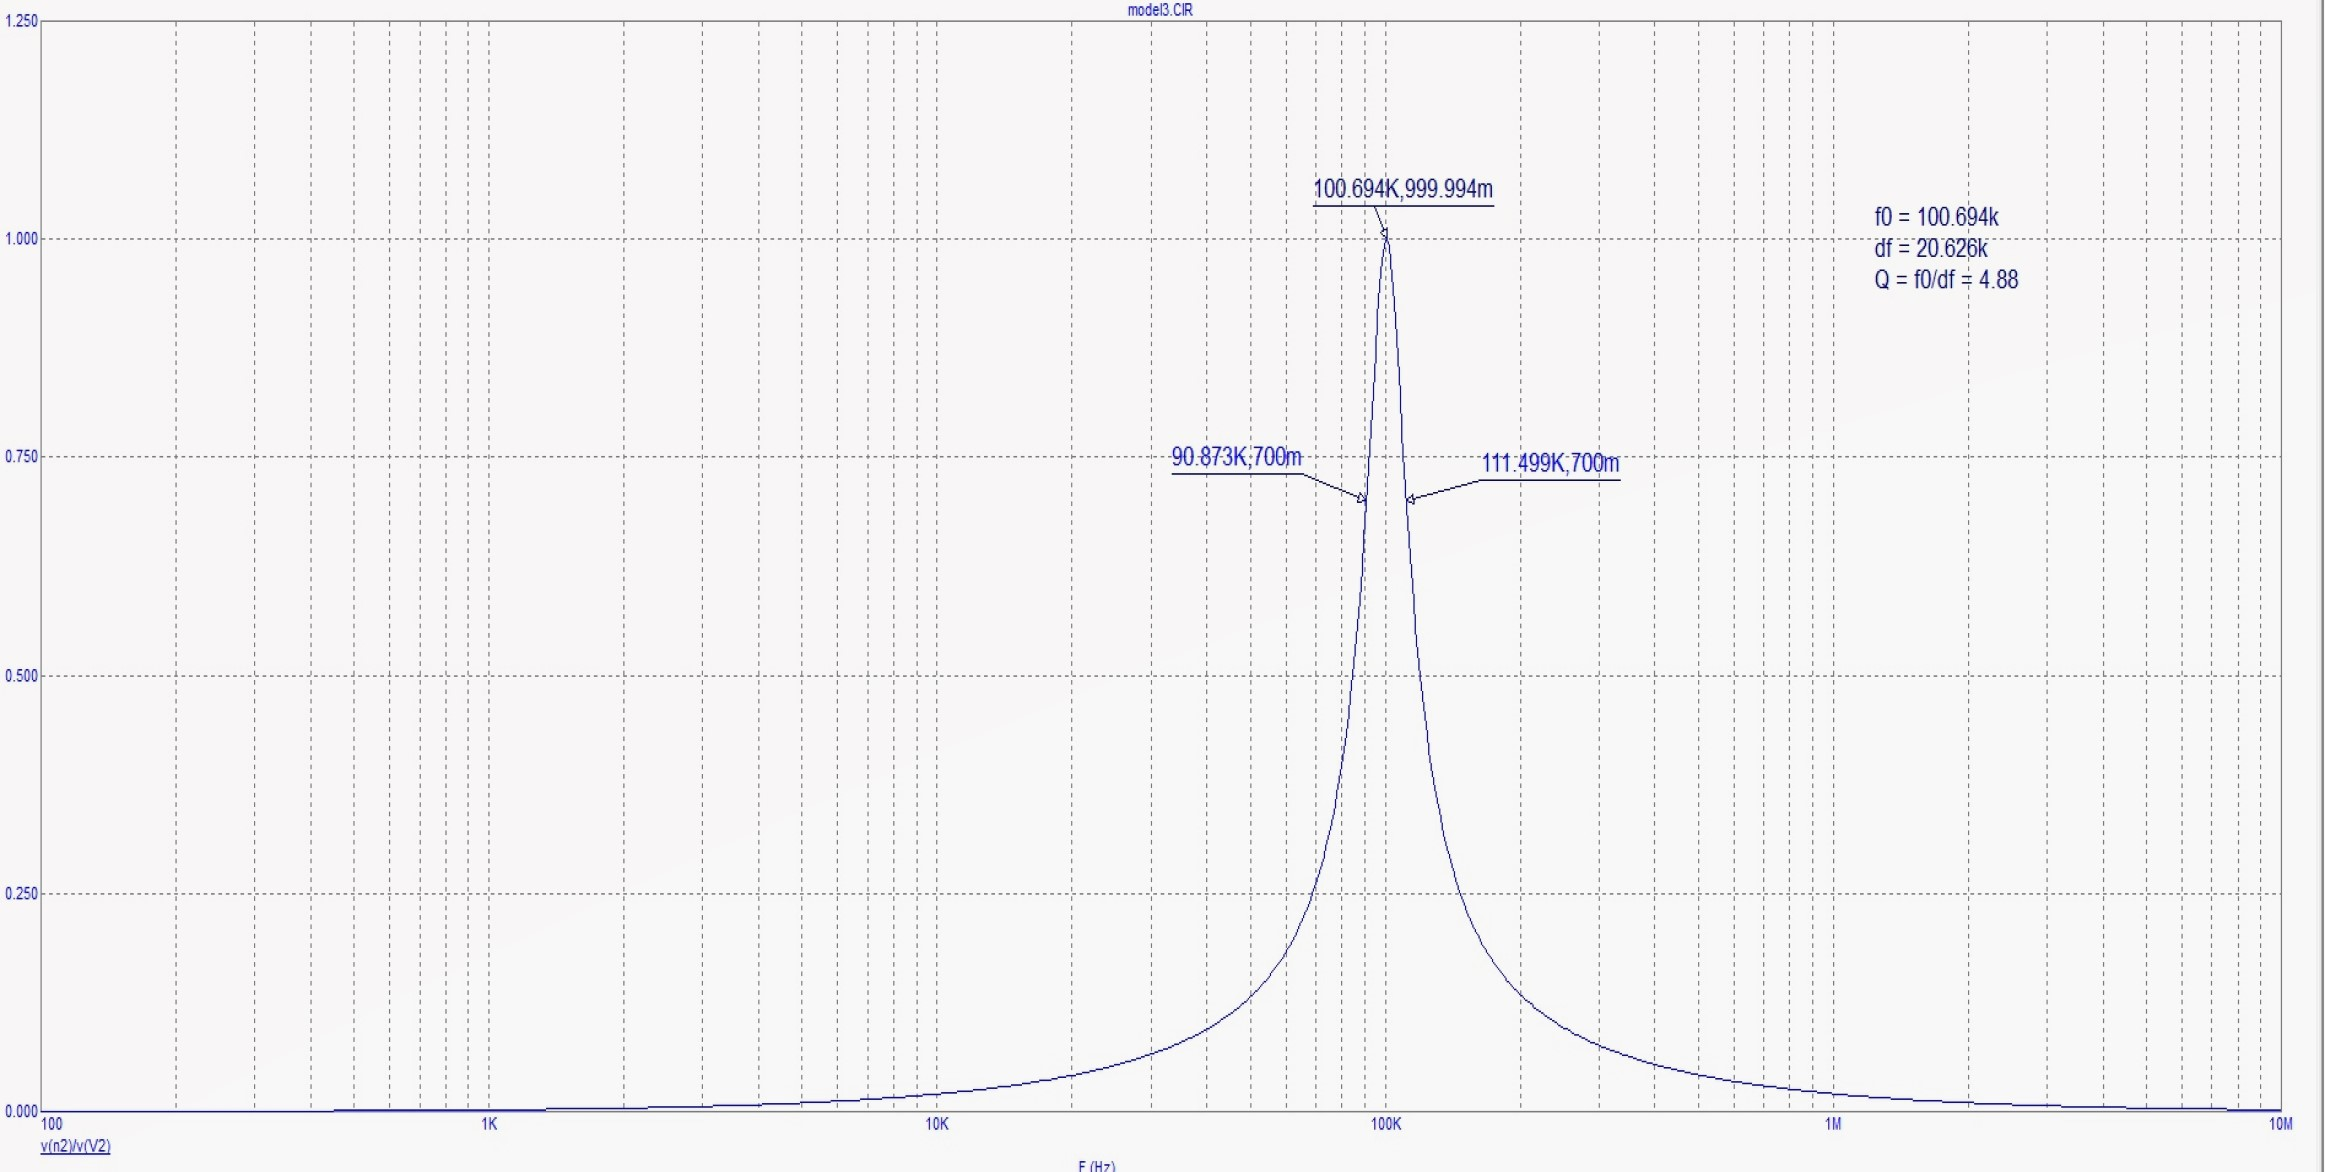
\includegraphics[width=1.1\linewidth]{3/3_2_1.jpg}
			\caption{Задание 3.2, пункт 1}
			\label{A}
\end{figure}

$ $

$\textbf{2.}$

Переключимся на шумовые графики. Измеряем шумовое напряжение $n_2$ в точке $f_0$, уровень шума на выходе.
Проверяем аналогичные условия как в 3.1 пункт 1.

Измерения:

$n_2 = 10.219n$

$\sigma = 1.82u$.

Проверка формулы дала такое же значение шума.


\begin{figure}[h!]
			\centering
			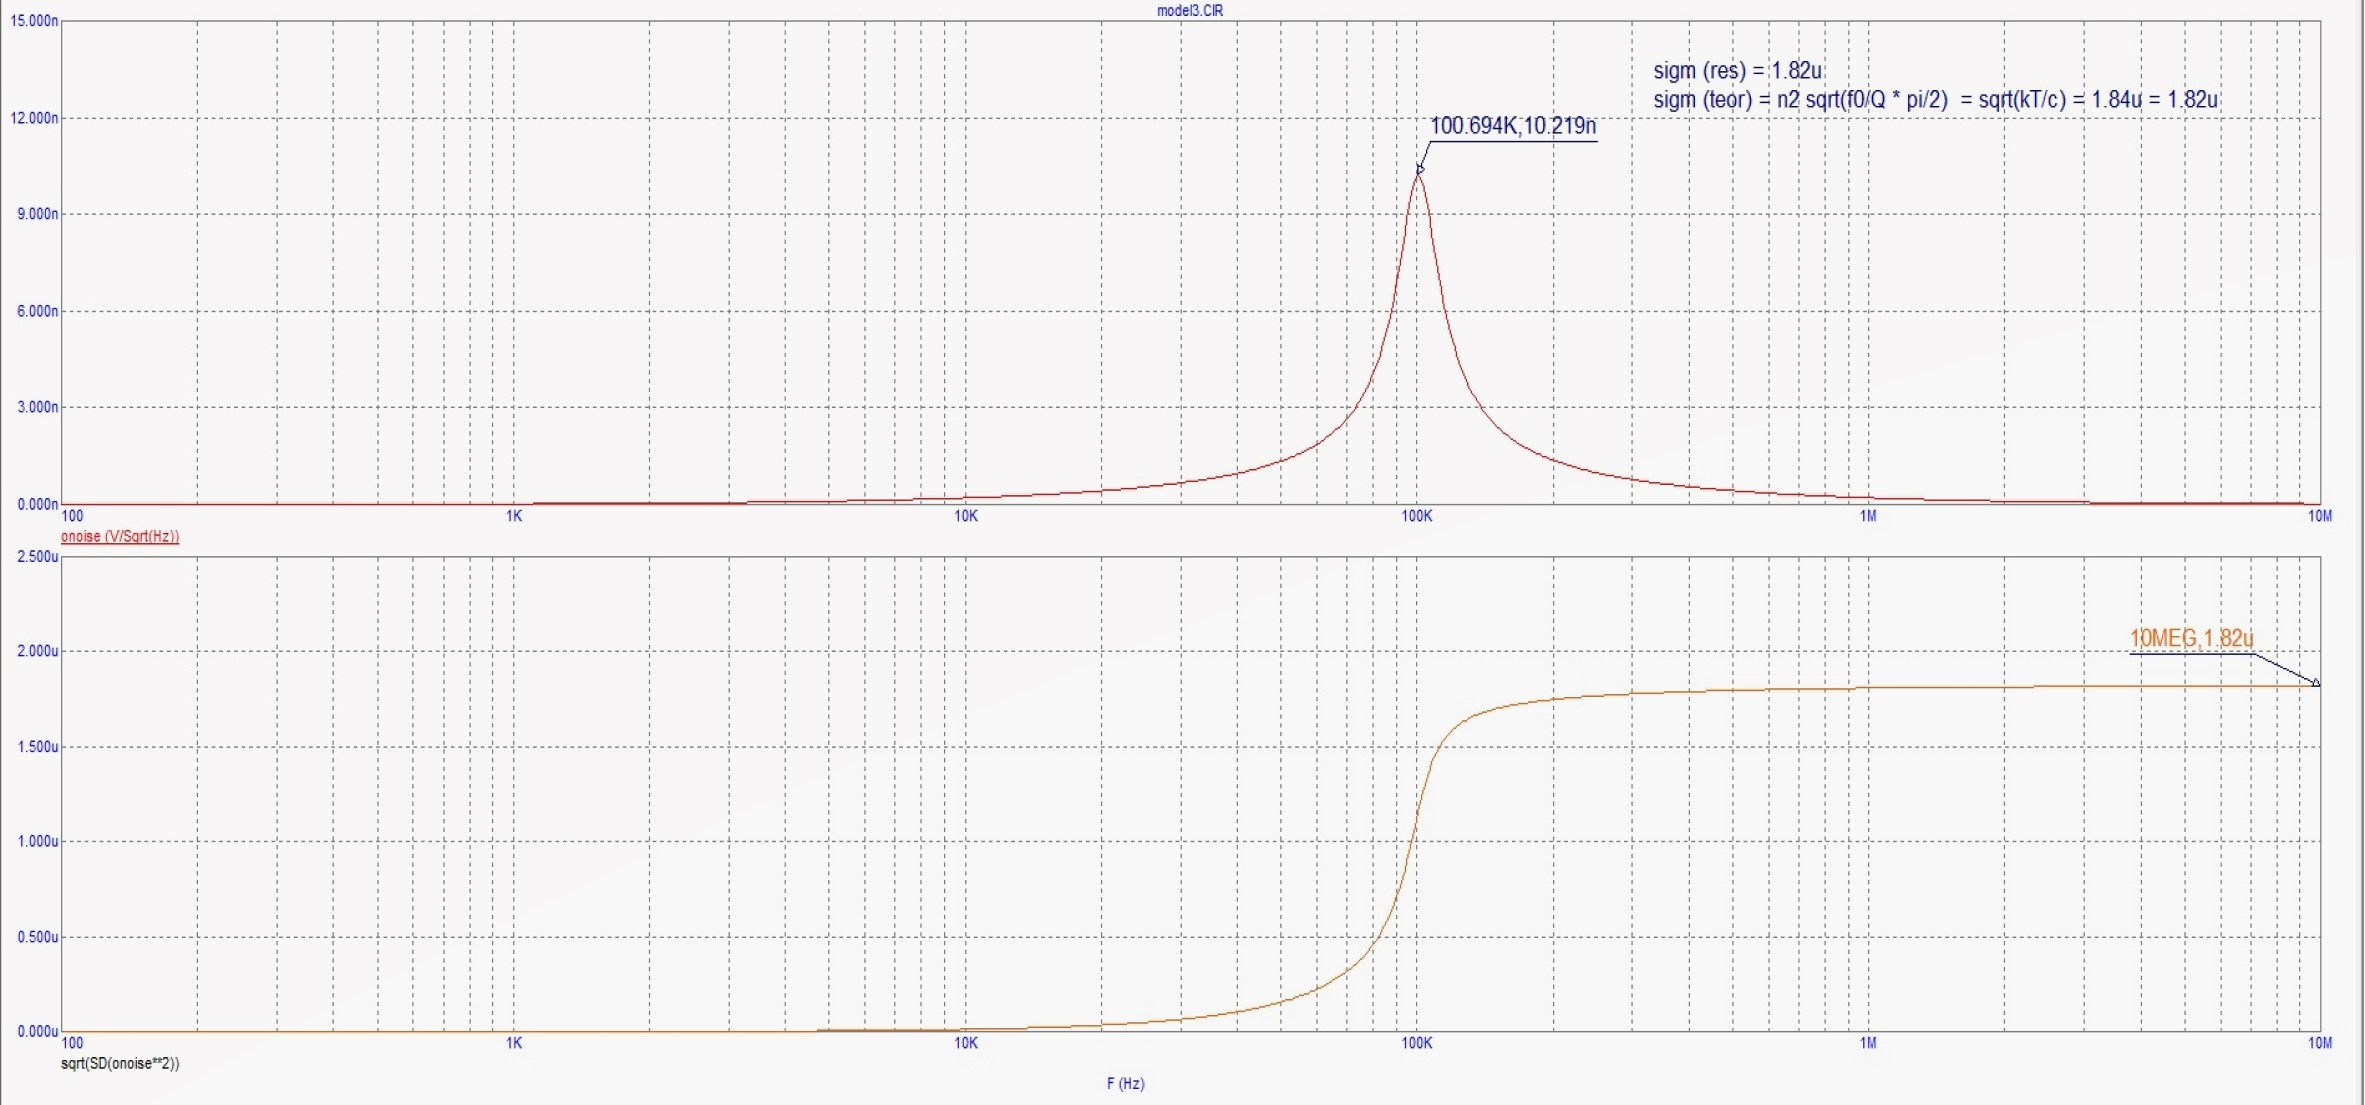
\includegraphics[width=1.1\linewidth]{3/3_2_2.jpg}
			\caption{Задание 3.2, пункт 2}
			\label{A}
\end{figure}


$\textbf{3.}$


Варьирование $R_2[2.3k, 10.3k | 4k]$.
Снимаем зависимость шумового напряжения от $R_2$. Соответственные кривые подписаны на графике.

\begin{figure}[h!]
			\centering
			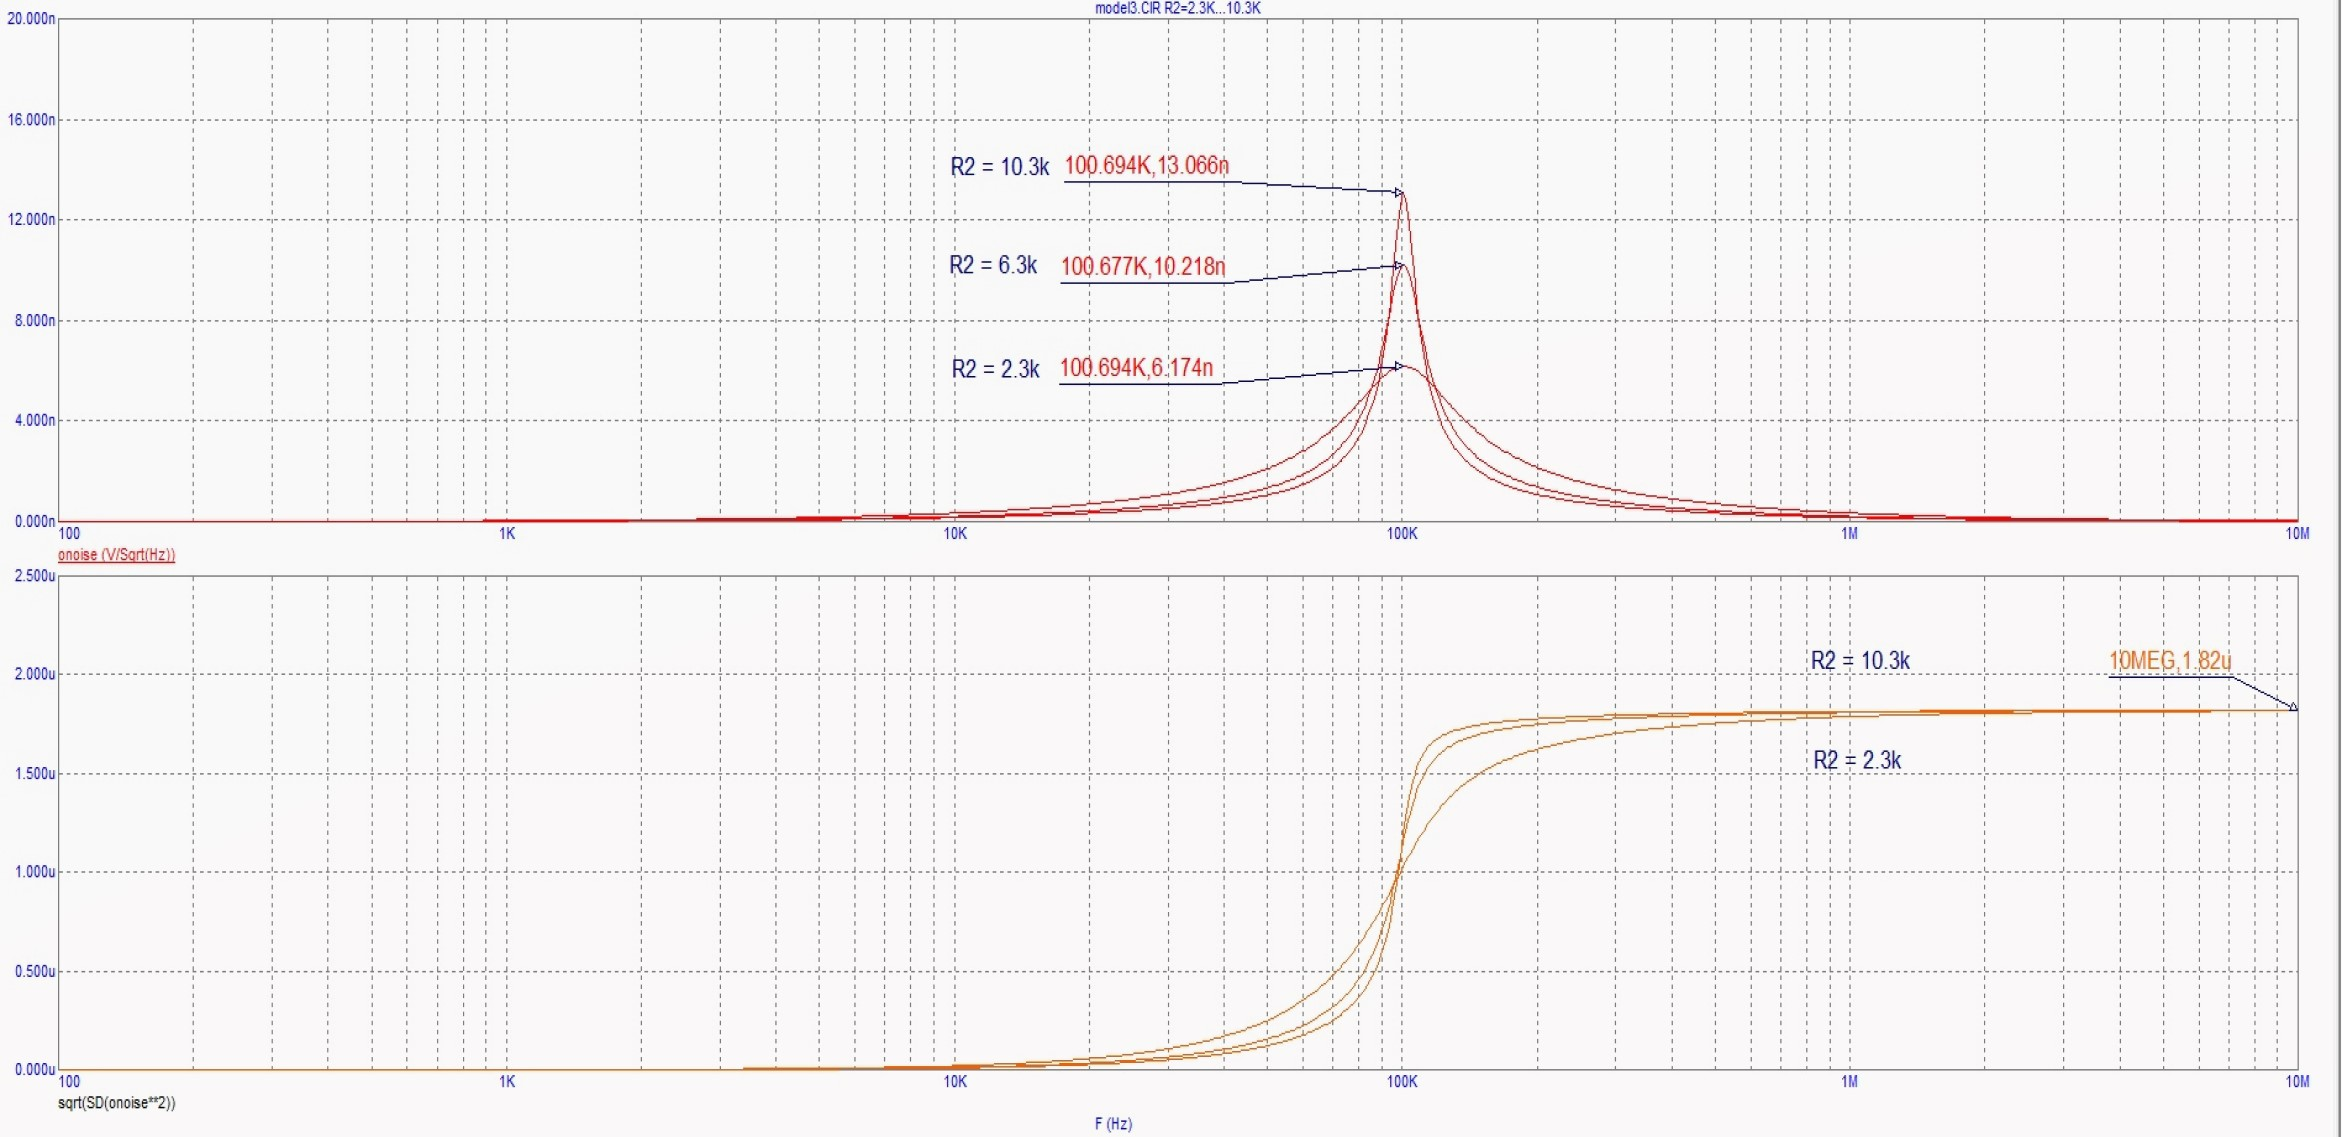
\includegraphics[width=1.1\linewidth]{3/3_2_5.jpg}
			\caption{Задание 3.2, пункт 3}
			\label{A}
\end{figure}

$\textbf{4.}$


Варьирование $С_2[0.75n, 1.75n | 0.5n]$.

Замечаем, что при мзенении емкости меняется частота резонанса, но шумовое напряжение $n_2$ на этой частоте остается прежним.
Снимаем зависимость уровня шума на выходе $\sigma$ от емкости.
Значение емкости указано для каждой кривой на скриншоте.

\begin{figure}[h!]
			\centering
			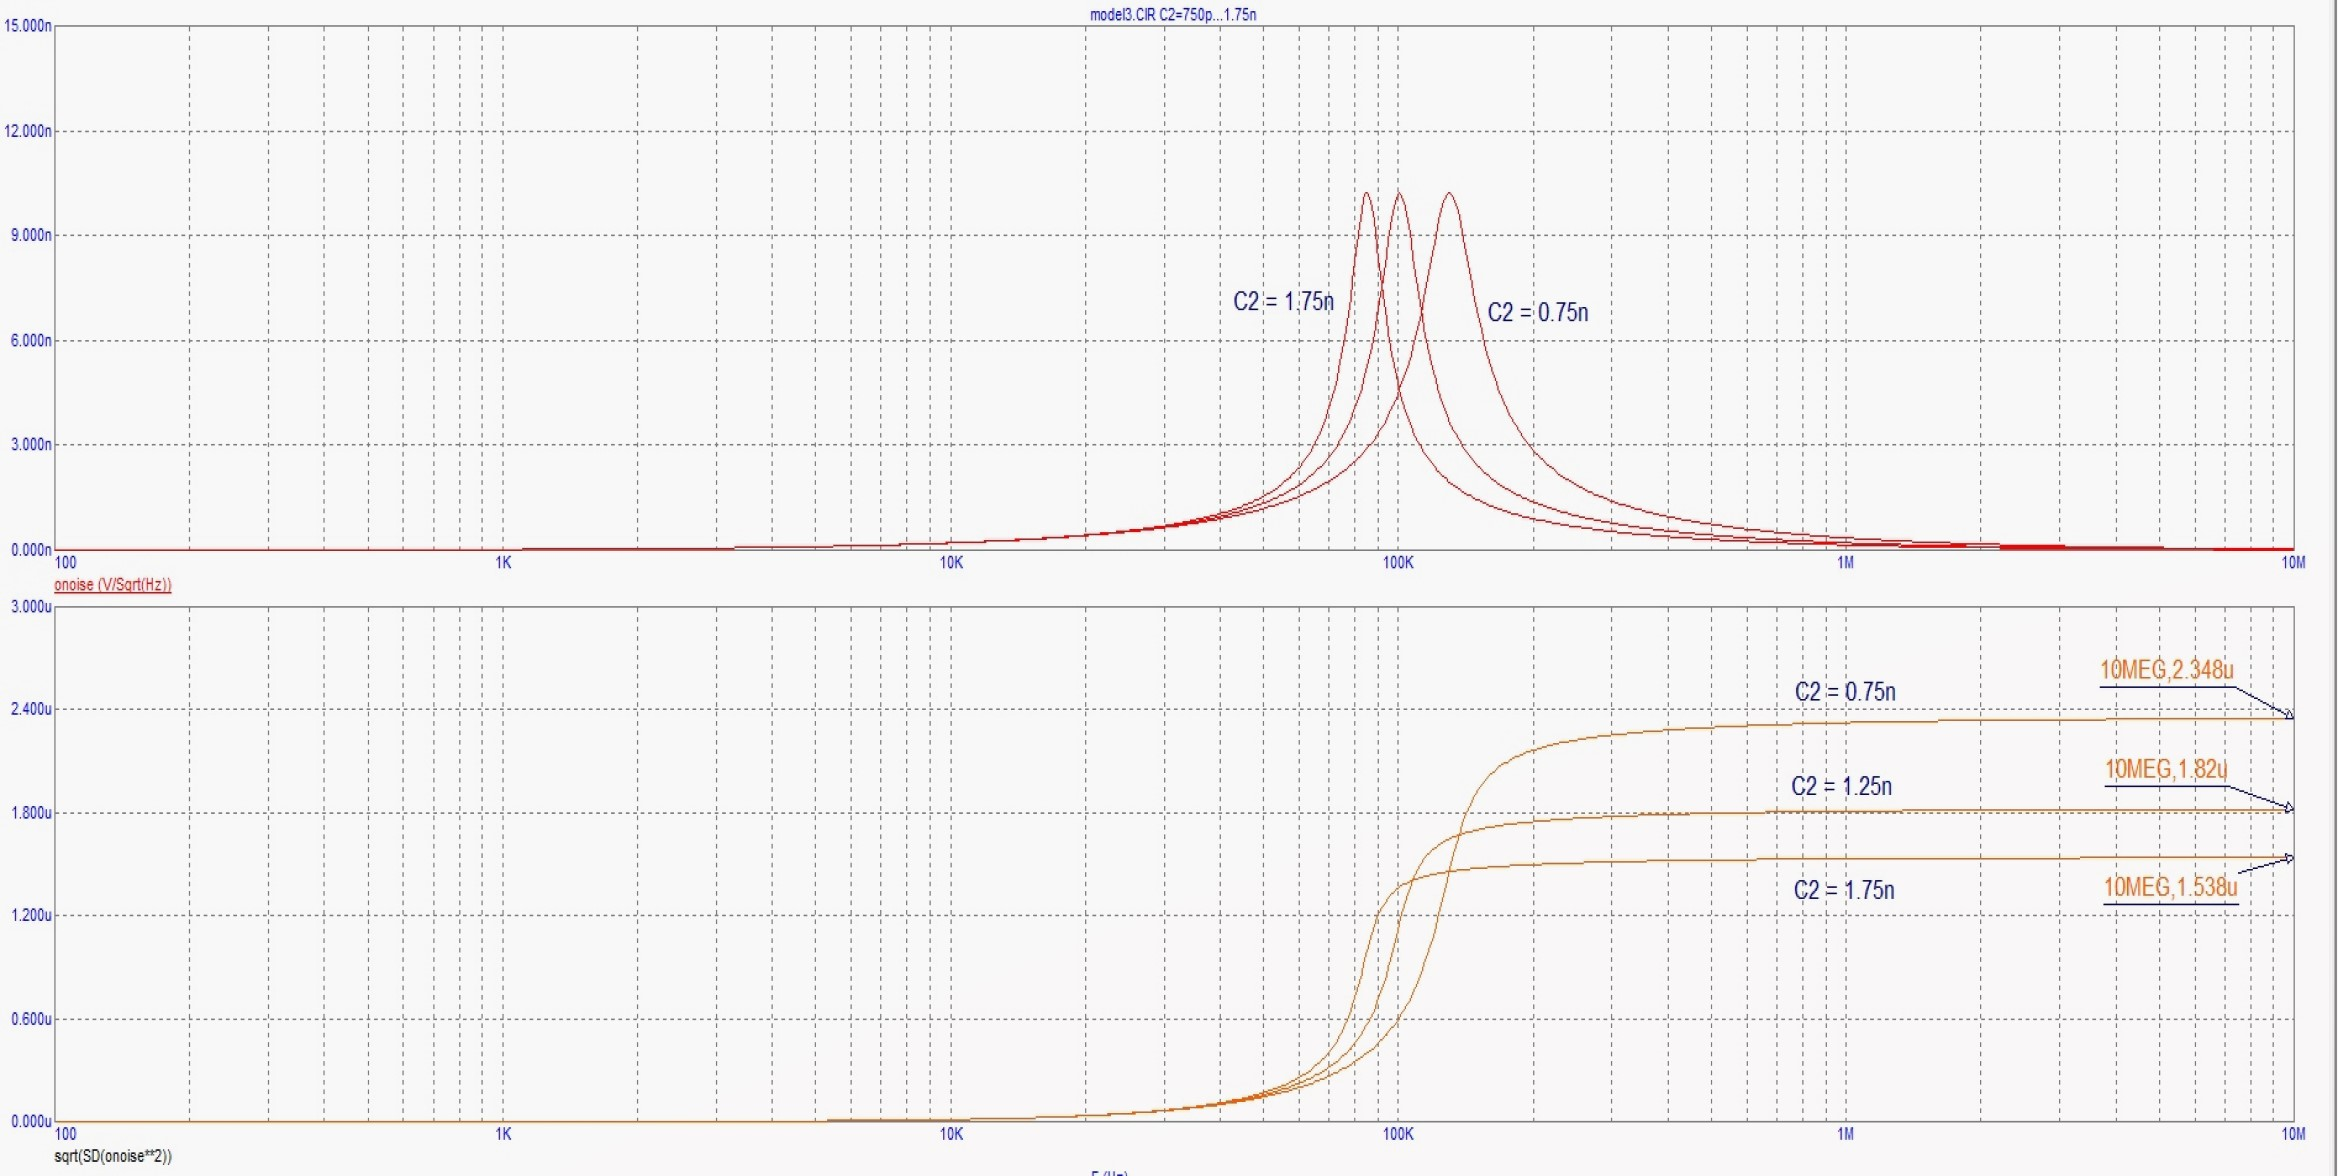
\includegraphics[width=1.1\linewidth]{3/3_2_3.jpg}
			\caption{Задание 3.2, пункт 4}
			\label{A}
\end{figure}


$\textbf{5.}$


Варьирование $L_2[1m, 3m | 1m]$.
Убеждаемся, что при изменении индуктивности сохраняются шумовое напряжение на частоте резонанса, уровень шума $\sigma$ на выходе. Для каждой кривой подписано соответственное значение индуктивности.

\begin{figure}[h!]
			\centering
			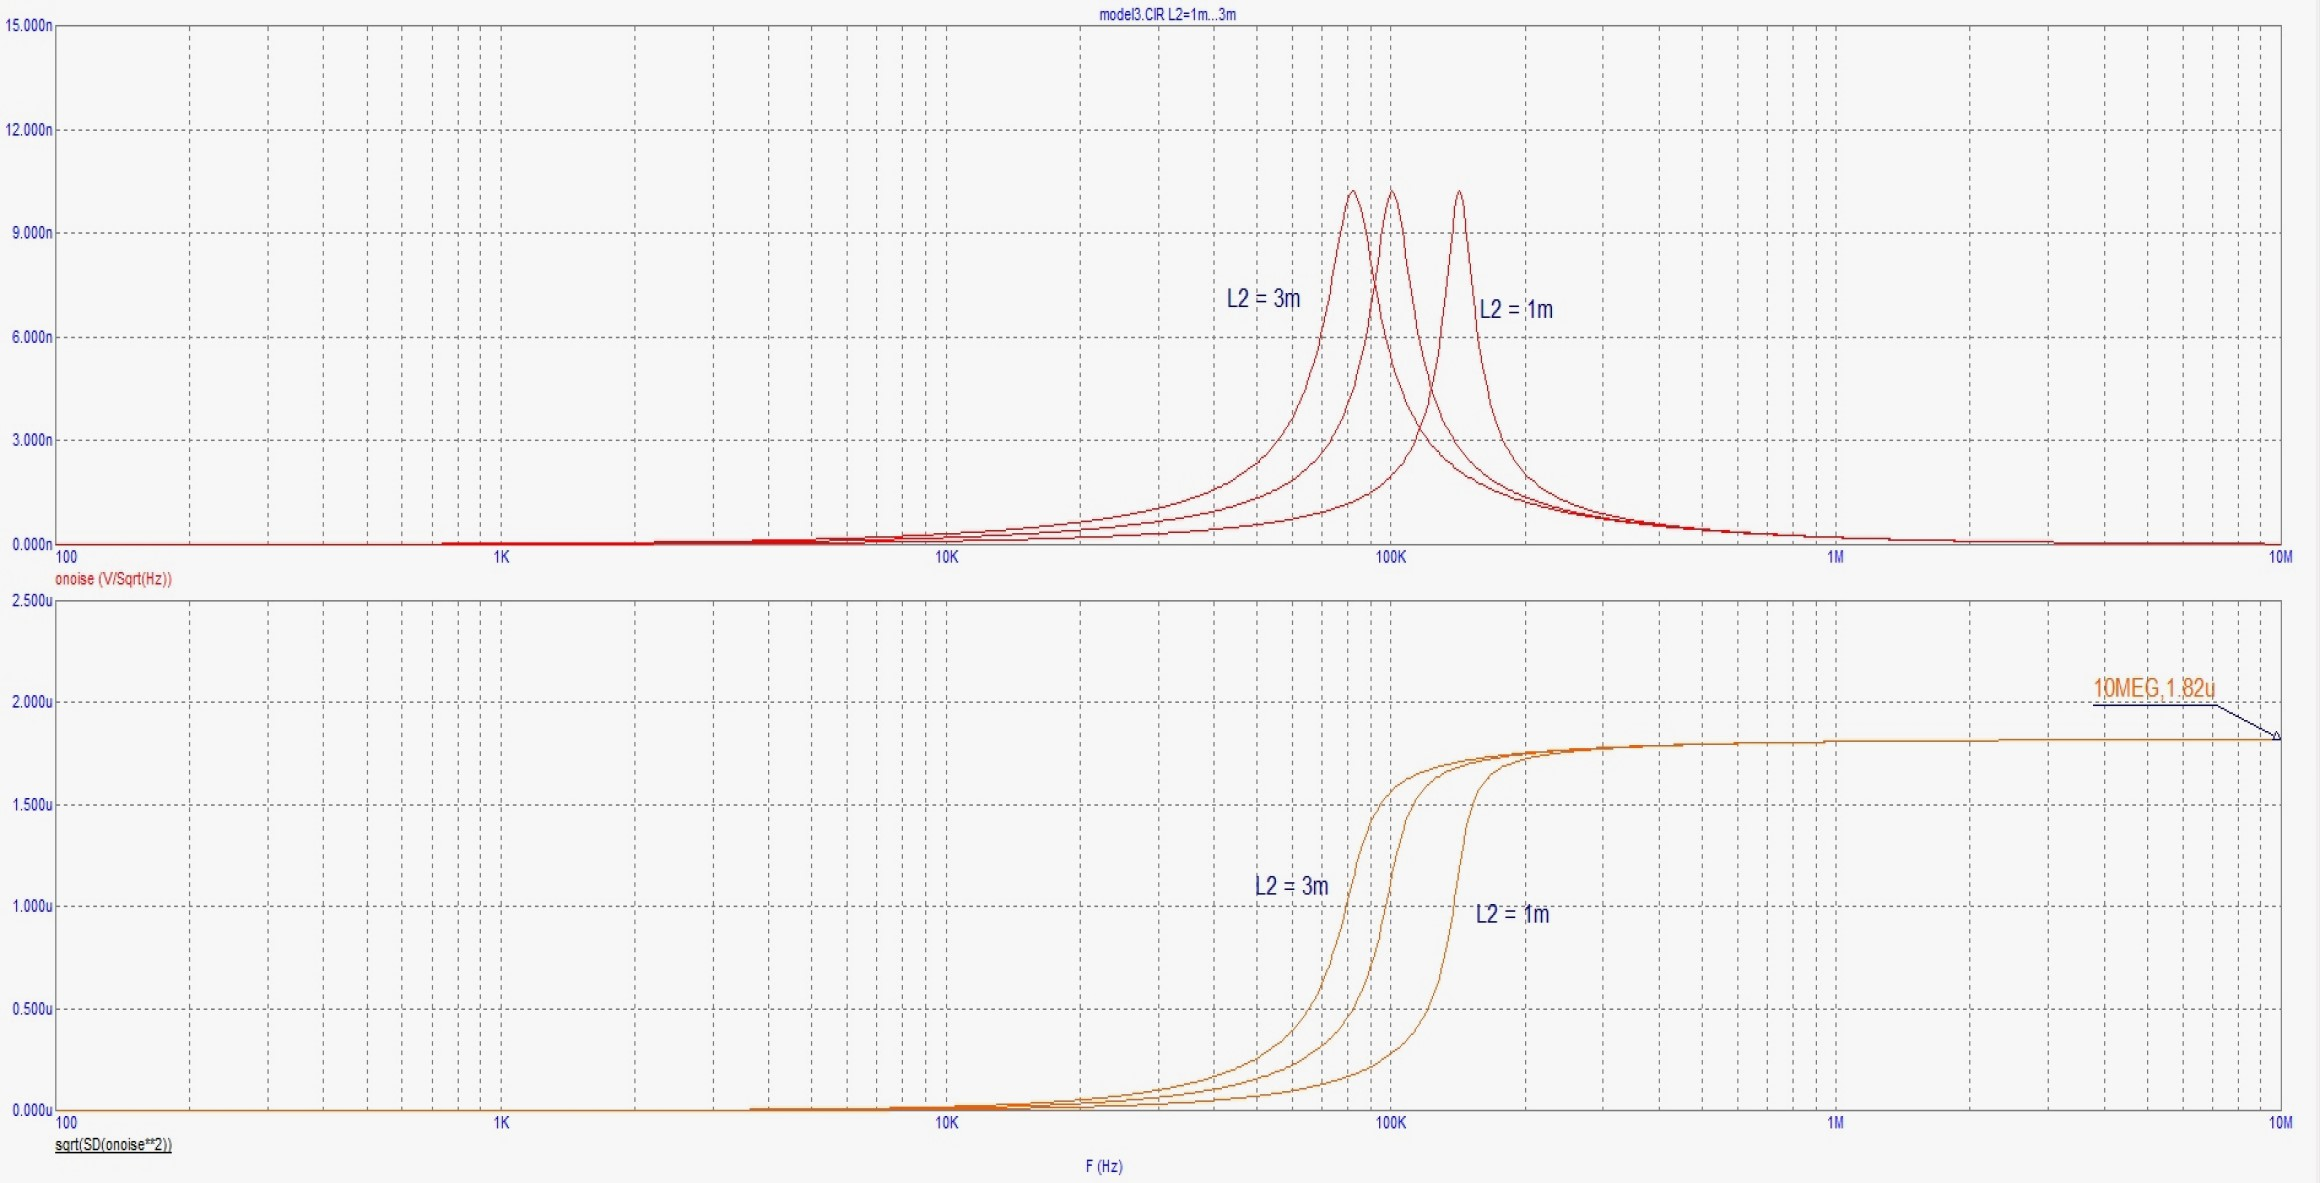
\includegraphics[width=1.1\linewidth]{3/3_2_4.jpg}
			\caption{Задание 3.2, пункт 5}
			\label{A}
\end{figure}

\subsection{Установить $\frac{V3}{n3}$ ($LC$--фильтр нижних частот)}

Рассматриваем LC - фильтр нижниъ частот.

$p = \frac{jf}{f_o}, f_0 = 100k, \rho = 1260, Q = \frac{1}{2\sigma} = 5$



$\textbf{1.} $


Измеряем шумовое напряжение $n_3$ в максимуме $f_0$, на частоте $f_0/10$, а так же уровень шума на выходе $\sigma$.
Проверим формулу $F_n = \frac{\pi\cdot f_0}{2\cdot Q}$.

Показания:

1) $f_0 = 99.54K \Rightarrow n_3 = 10.35n$

2) $f_0/10 = 9.95 \Rightarrow n_3 = 2.055n$

Напряжение шума на выходе:

$\sigma = 1.82u$.

Оценка шумовой полосы $F_n$ и проверка форумлы:

3) $F_{n_{theor}} = 31.3k$

4) $F_{n_{pract}} = (\frac{\sigma}{n_3})^{2} = 30.9k$

\begin{figure}[h!]
			\centering
			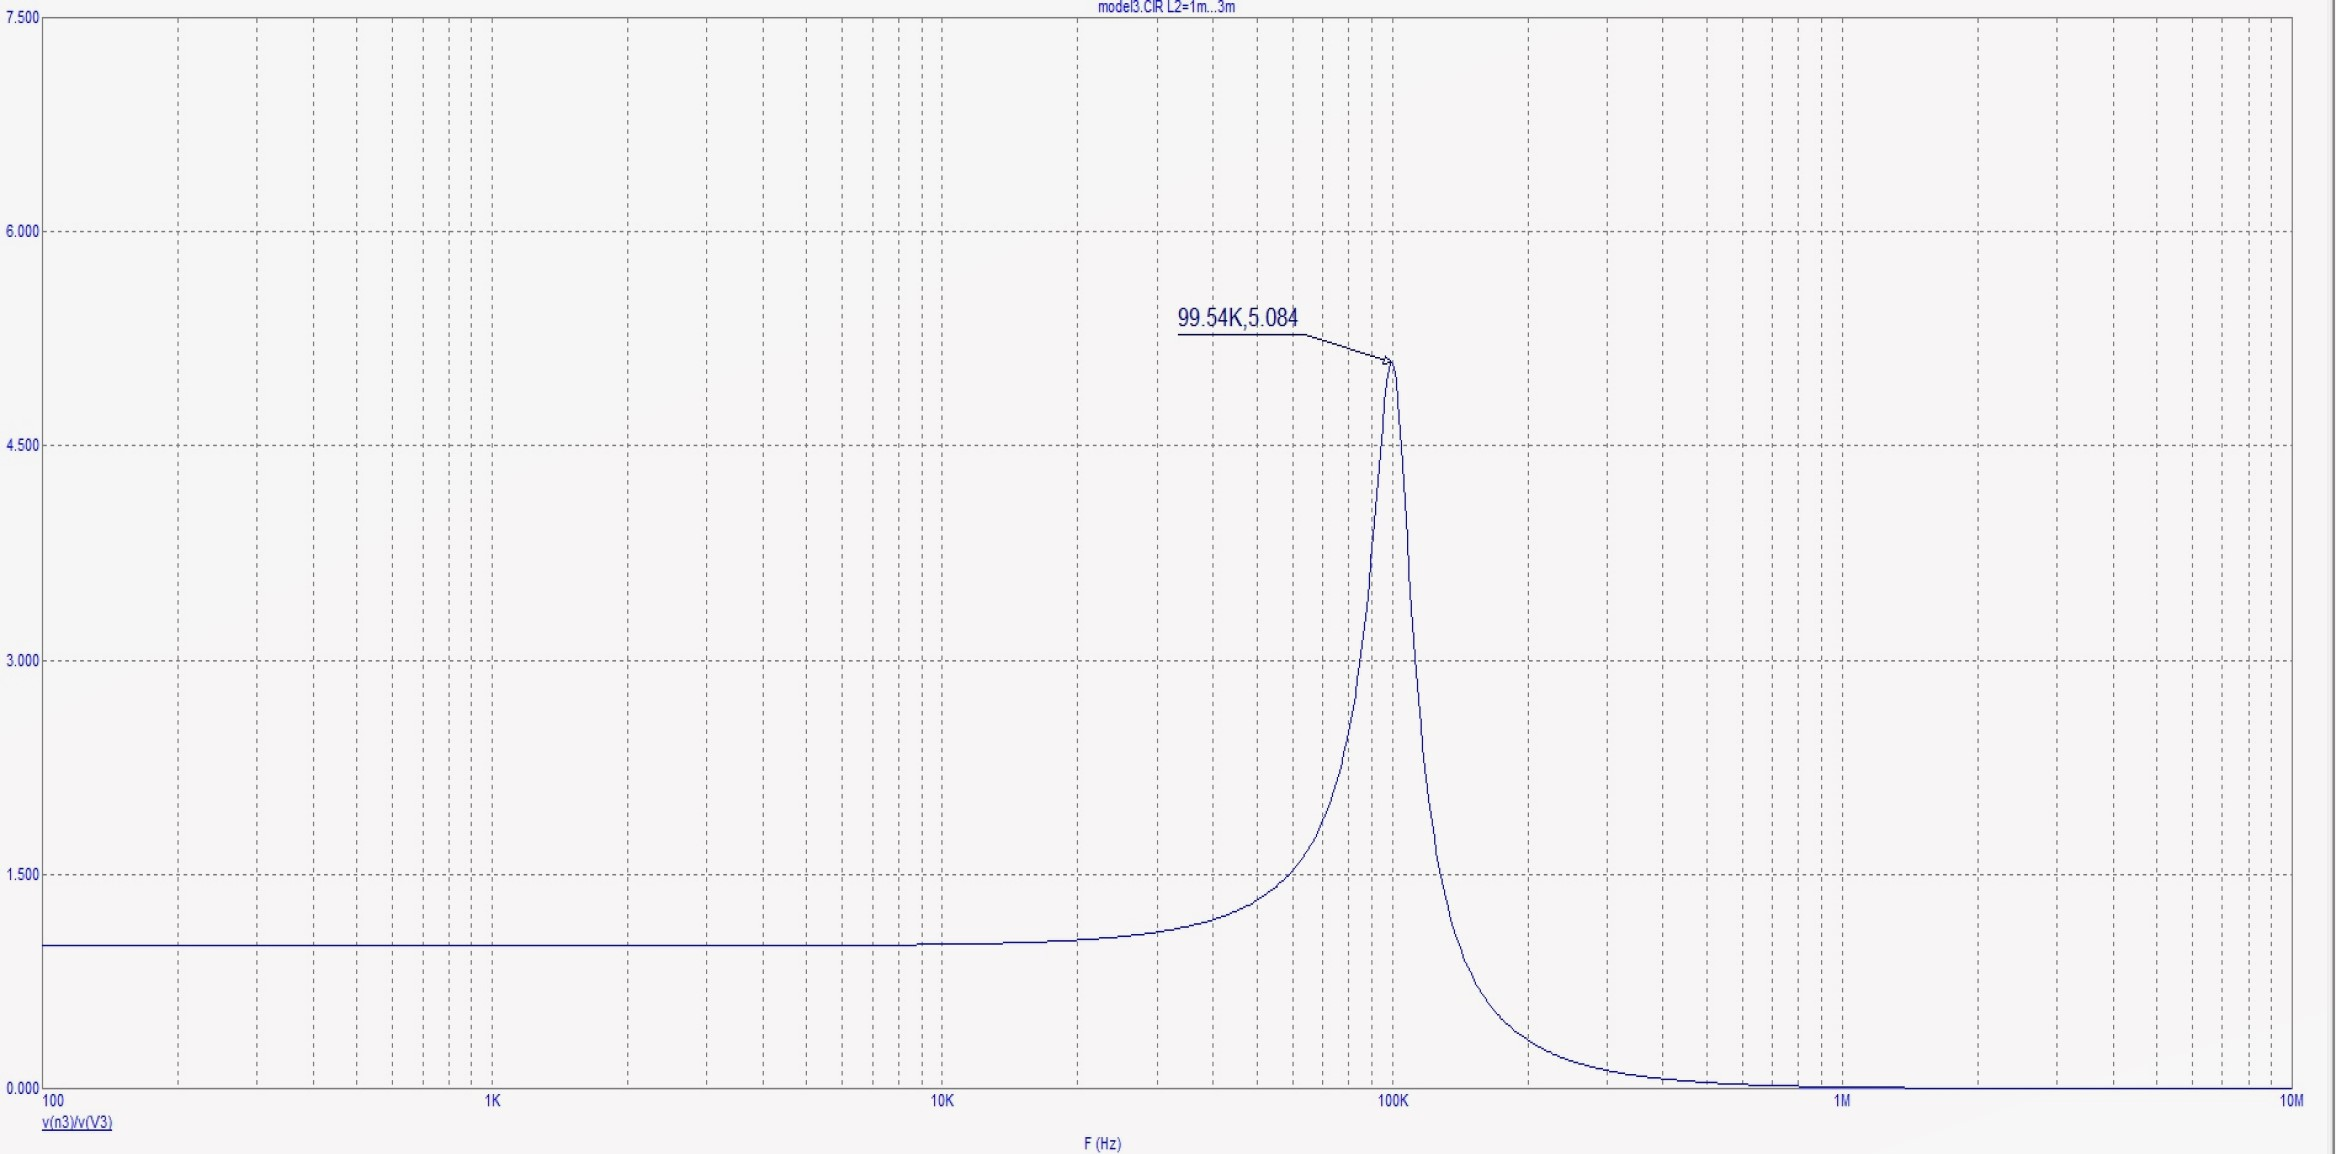
\includegraphics[width=1.1\linewidth]{3/3_3_1.jpg}
			\caption{Задание 3.3, пункт 1}
			\label{A}
\end{figure}



\begin{figure}[h!]
			\centering
			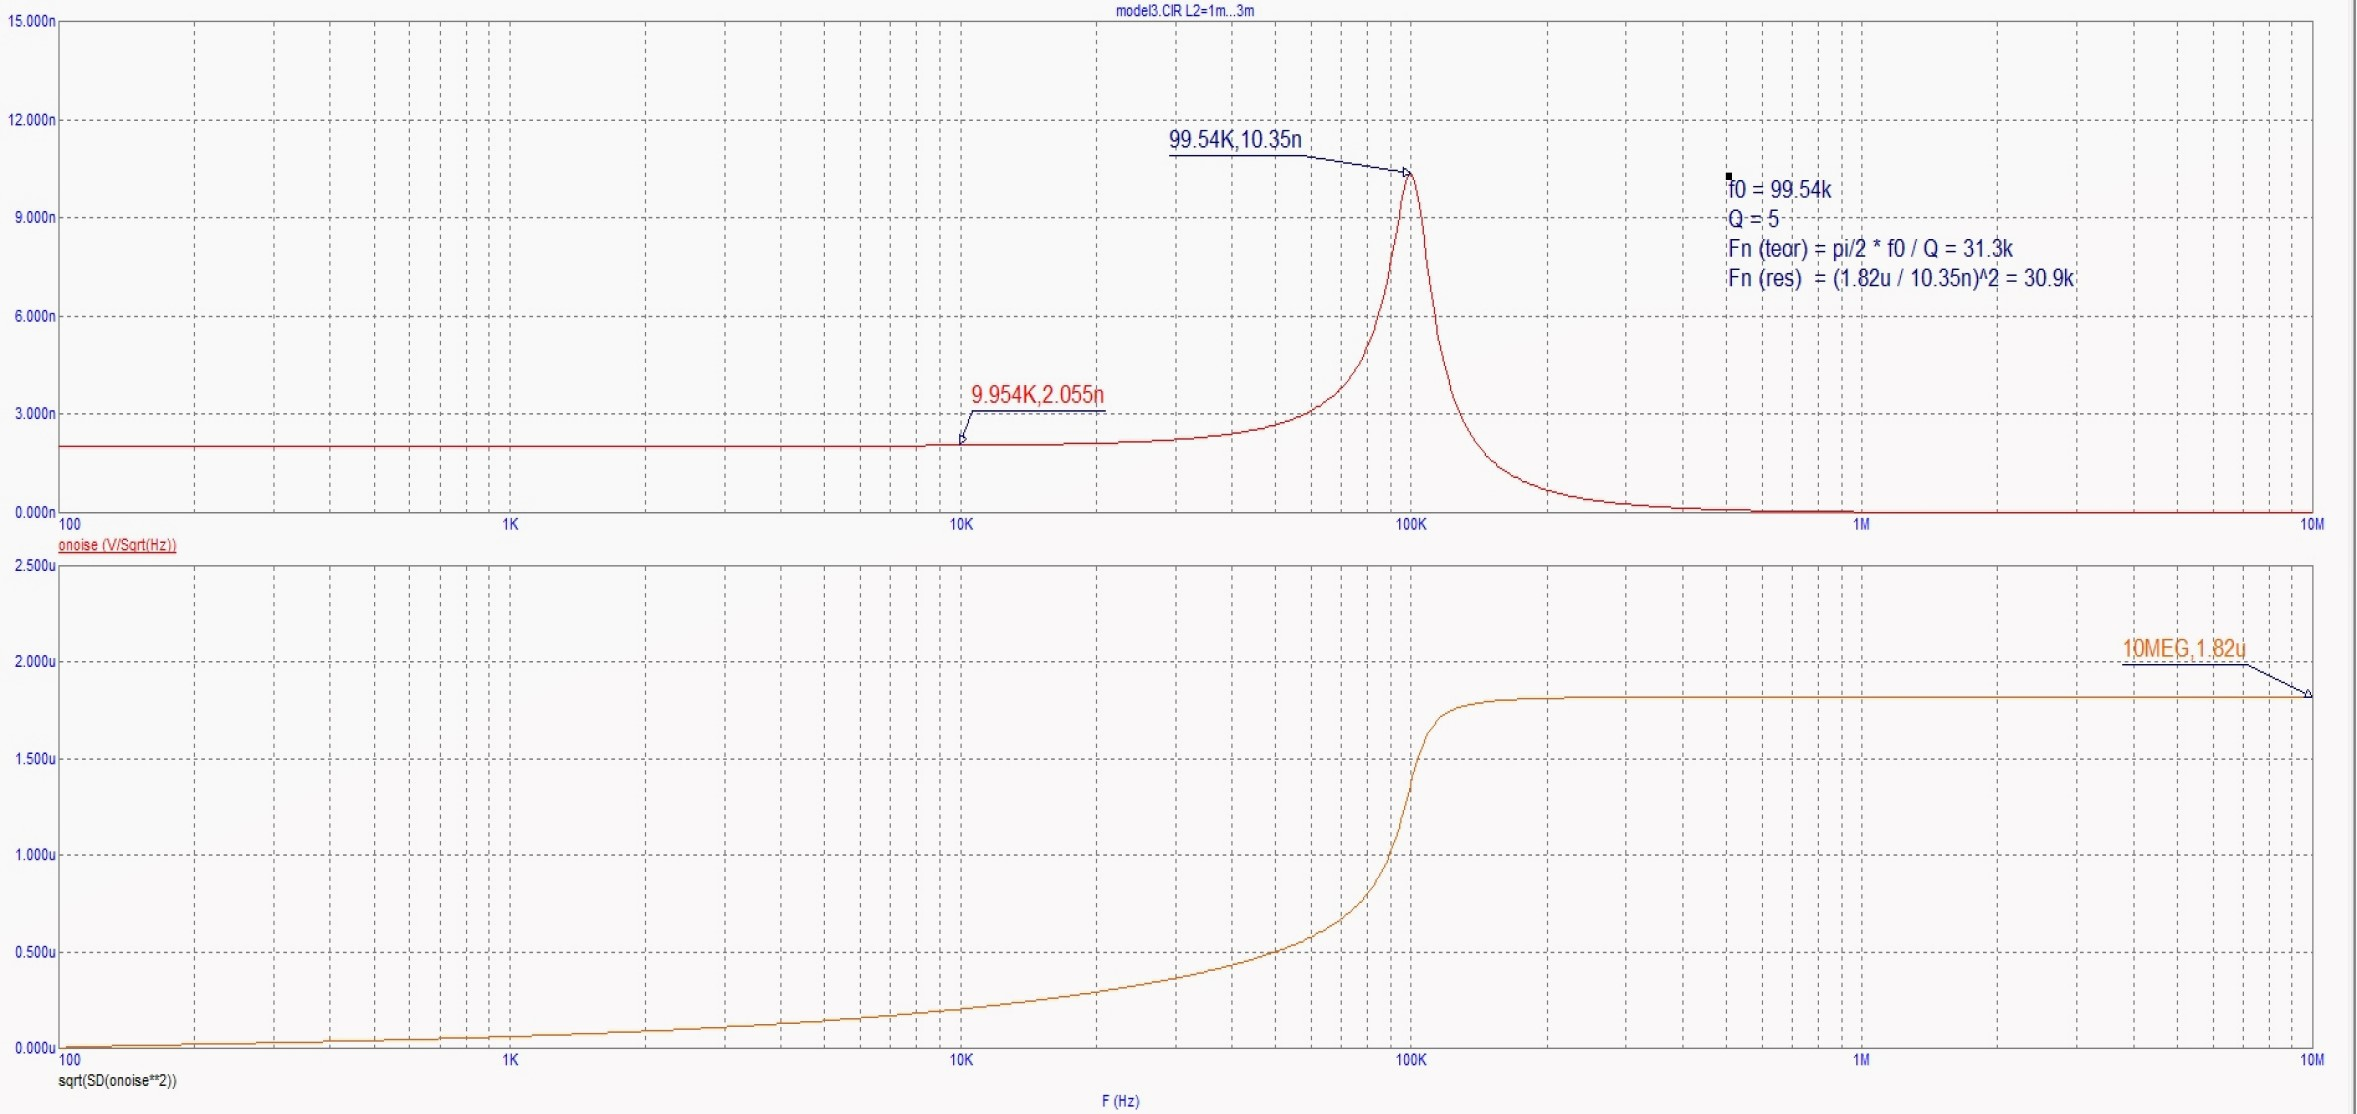
\includegraphics[width=1.1\linewidth]{3/3_3_2.jpg}
			\caption{Задание 3.3, пункт 1}
			\label{A}
\end{figure}



$\textbf{2.} $

Варьирование $R_3[100, 400 | 150]$.

Варьирование $C_3[0.75n, 1.75n | 0.5n]$.

Варьирование $L_3[1m, 3m | 1m]$.

Фиксируем зависимости $n_3(f_0), \: n_3(f_0/10), \: \sigma$ от изменяемых параметров.


\begin{figure}[h!]
			\centering
			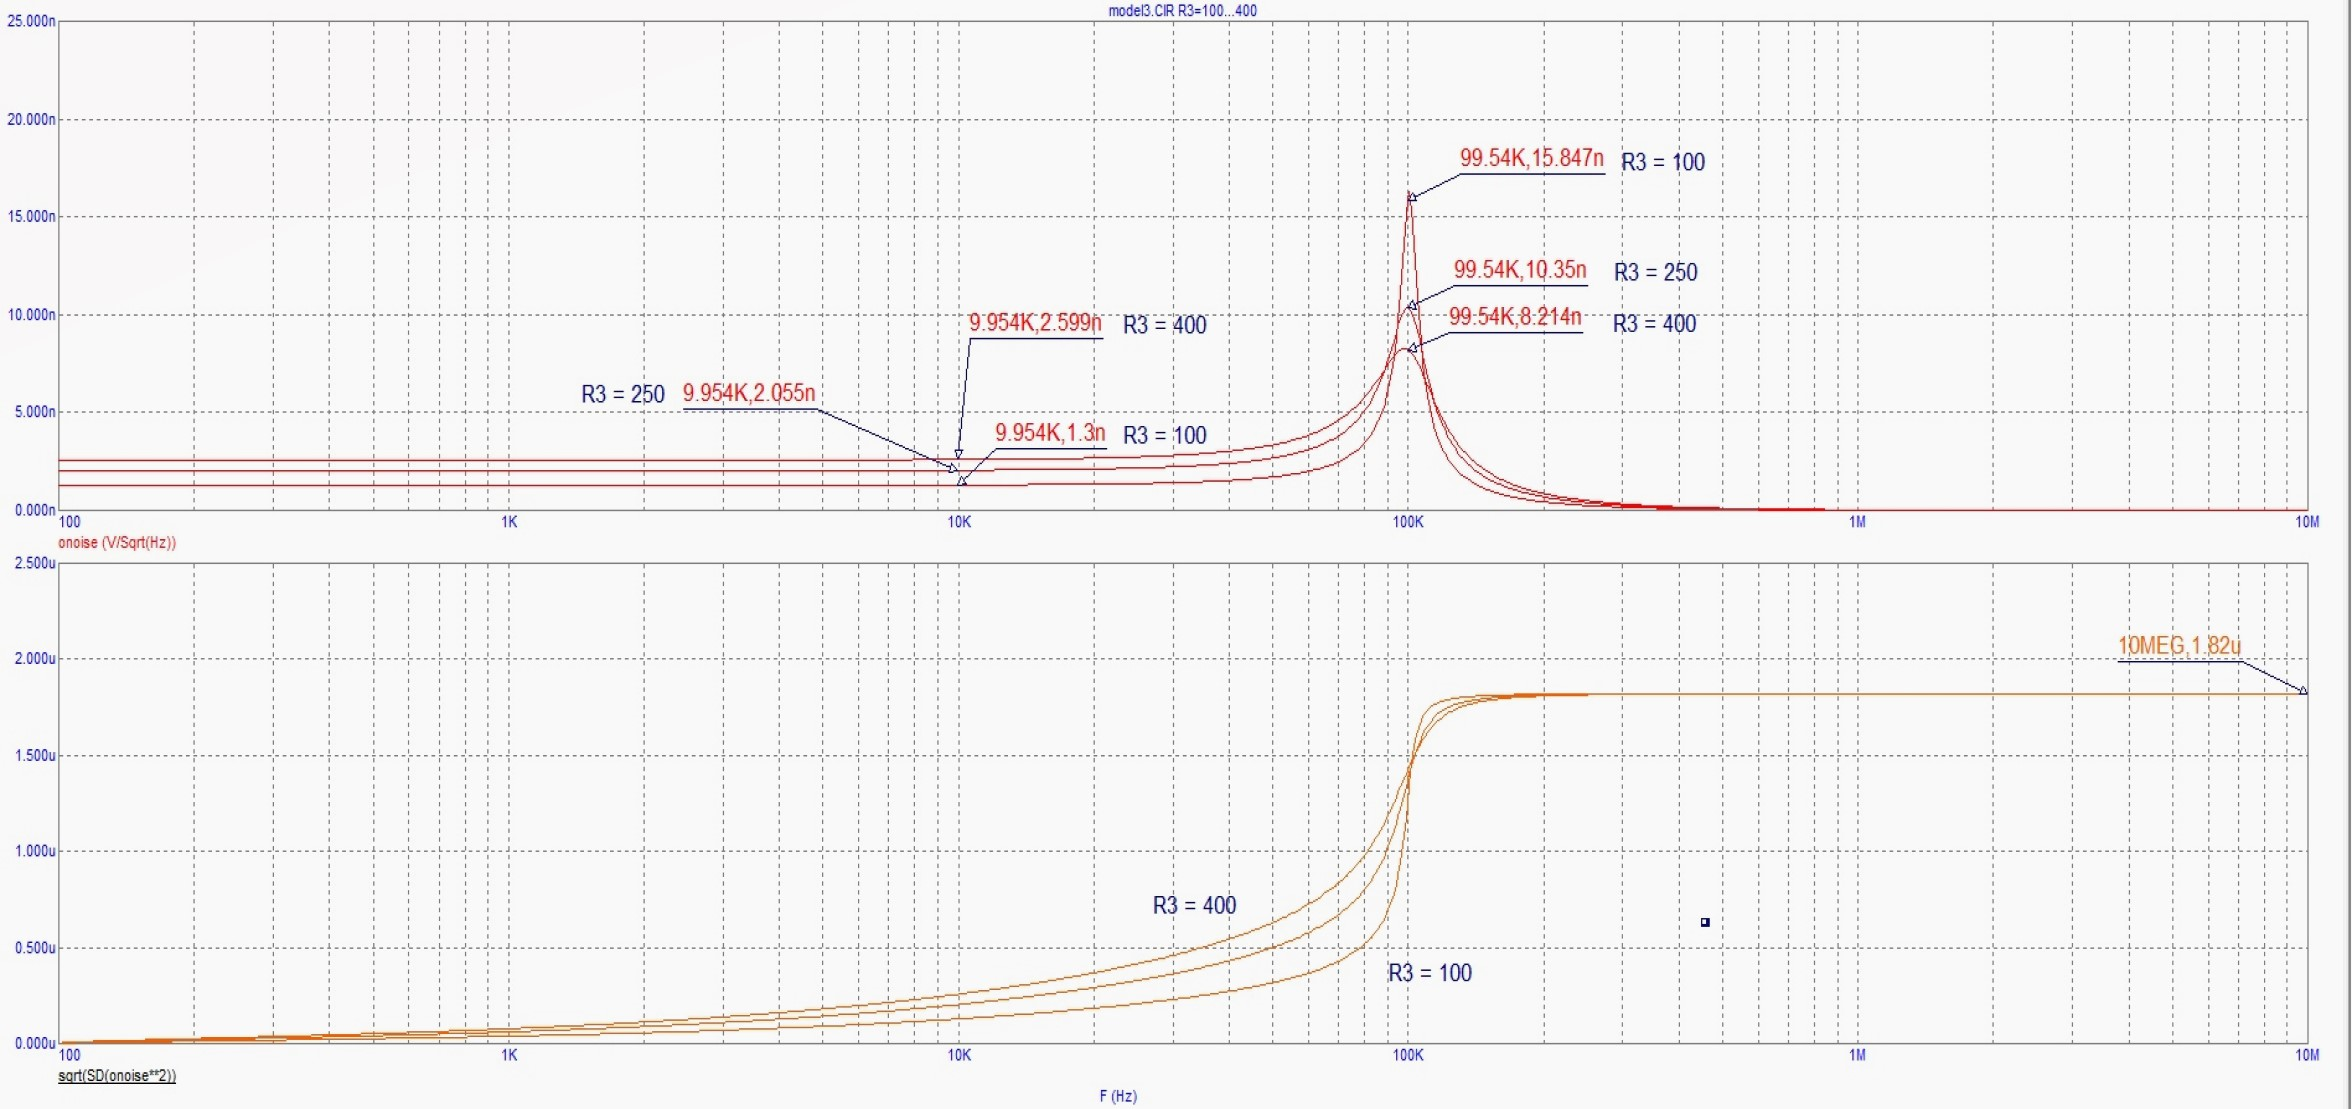
\includegraphics[width=1.1\linewidth]{3/3_3_5.jpg}
			\caption{Задание 3.3, пункт 2, варьирование R}
			\label{A}
\end{figure}



\begin{figure}[h!]
			\centering
			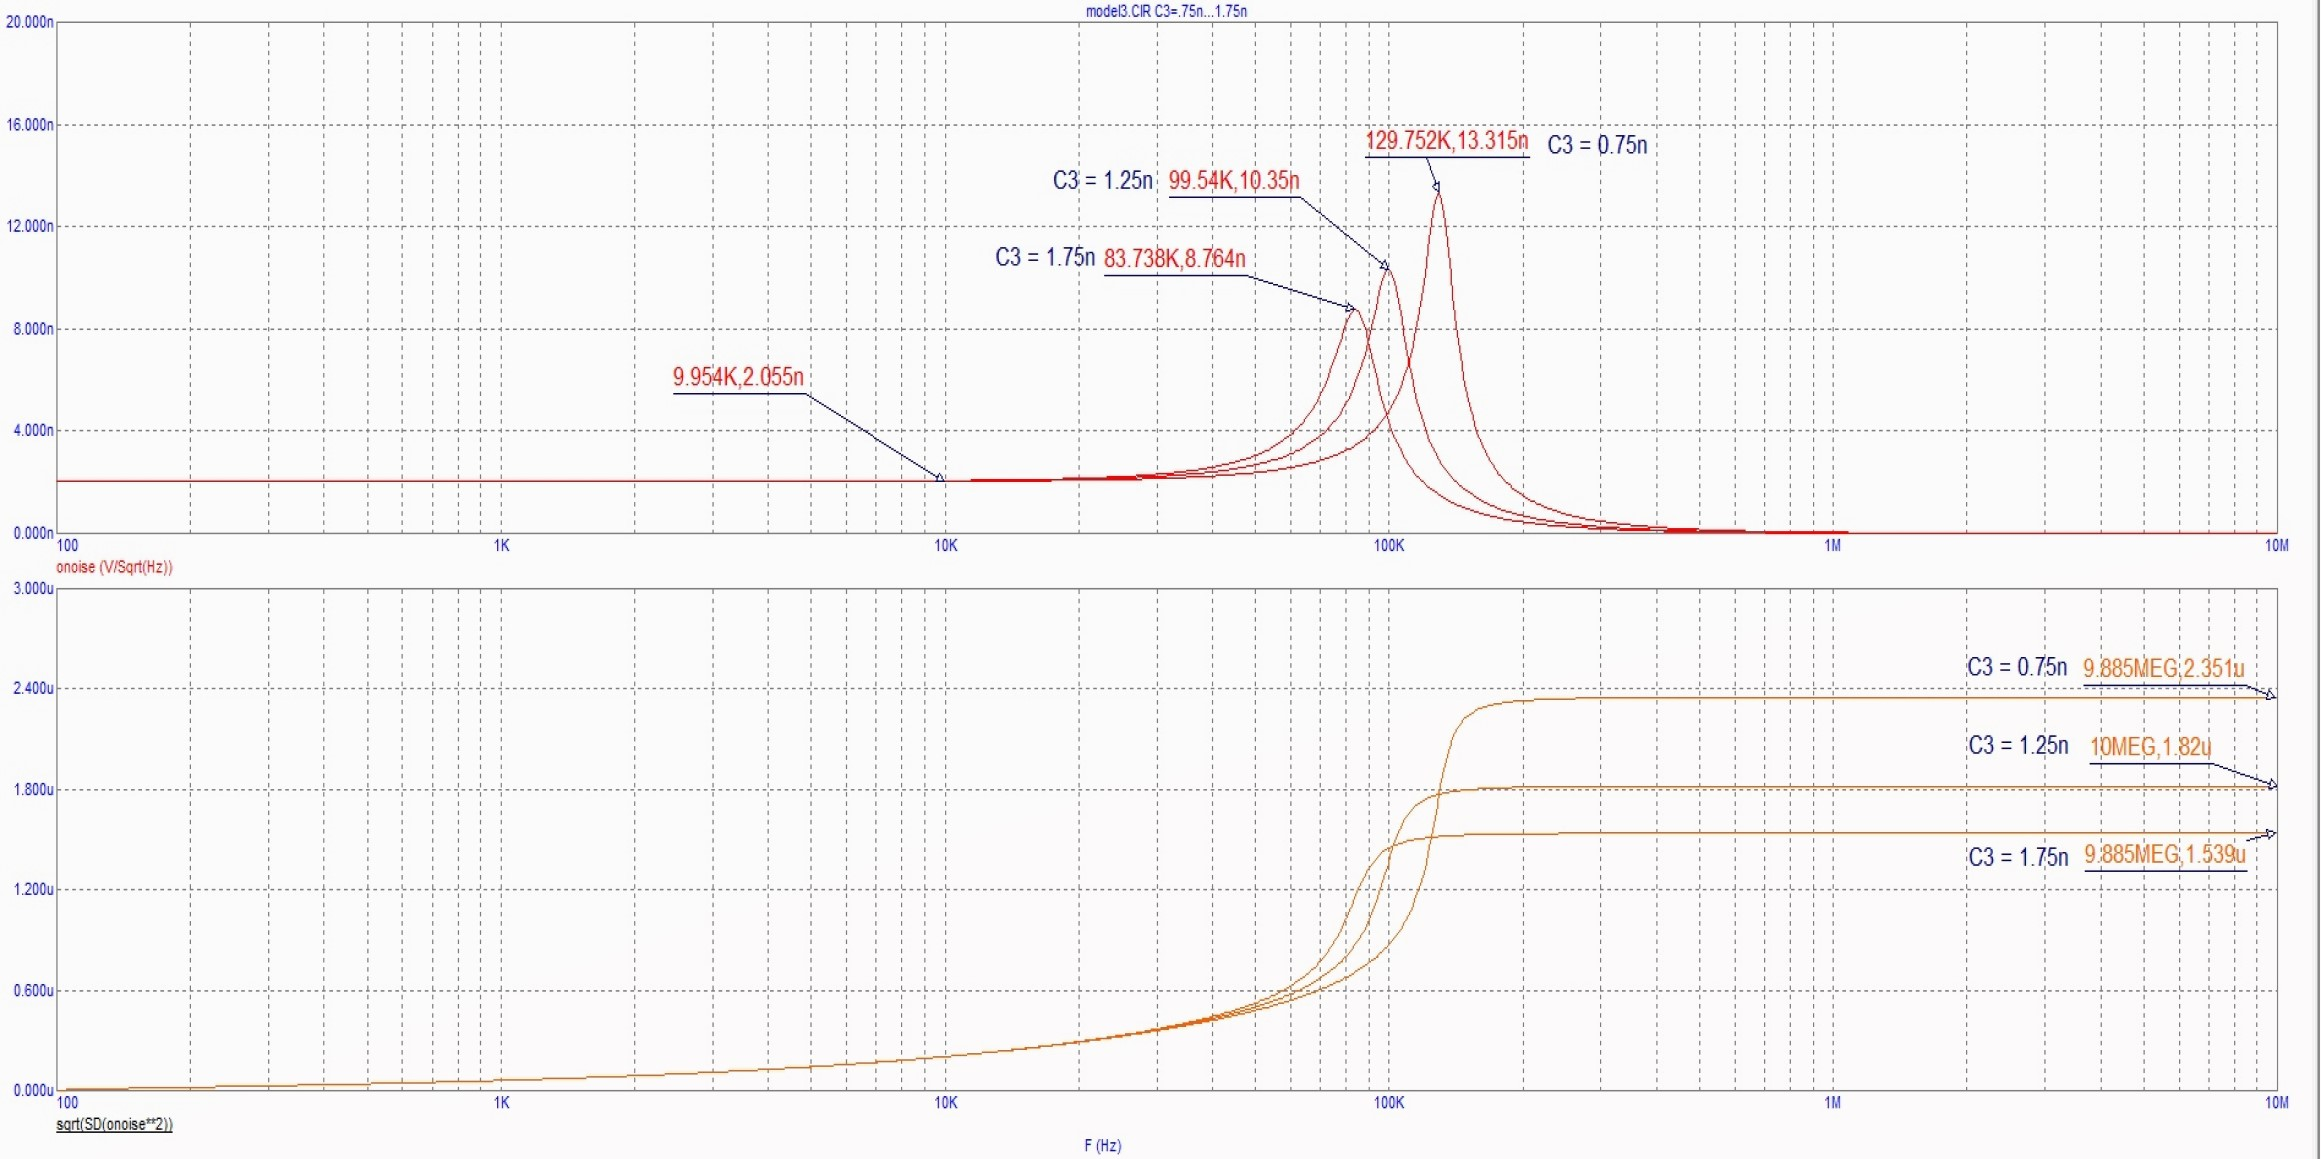
\includegraphics[width=1.1\linewidth]{3/3_3_3.jpg}
			\caption{Задание 3.3, пункт 2, варьирование C}
			\label{A}
\end{figure}



\begin{figure}[h!]
			\centering
			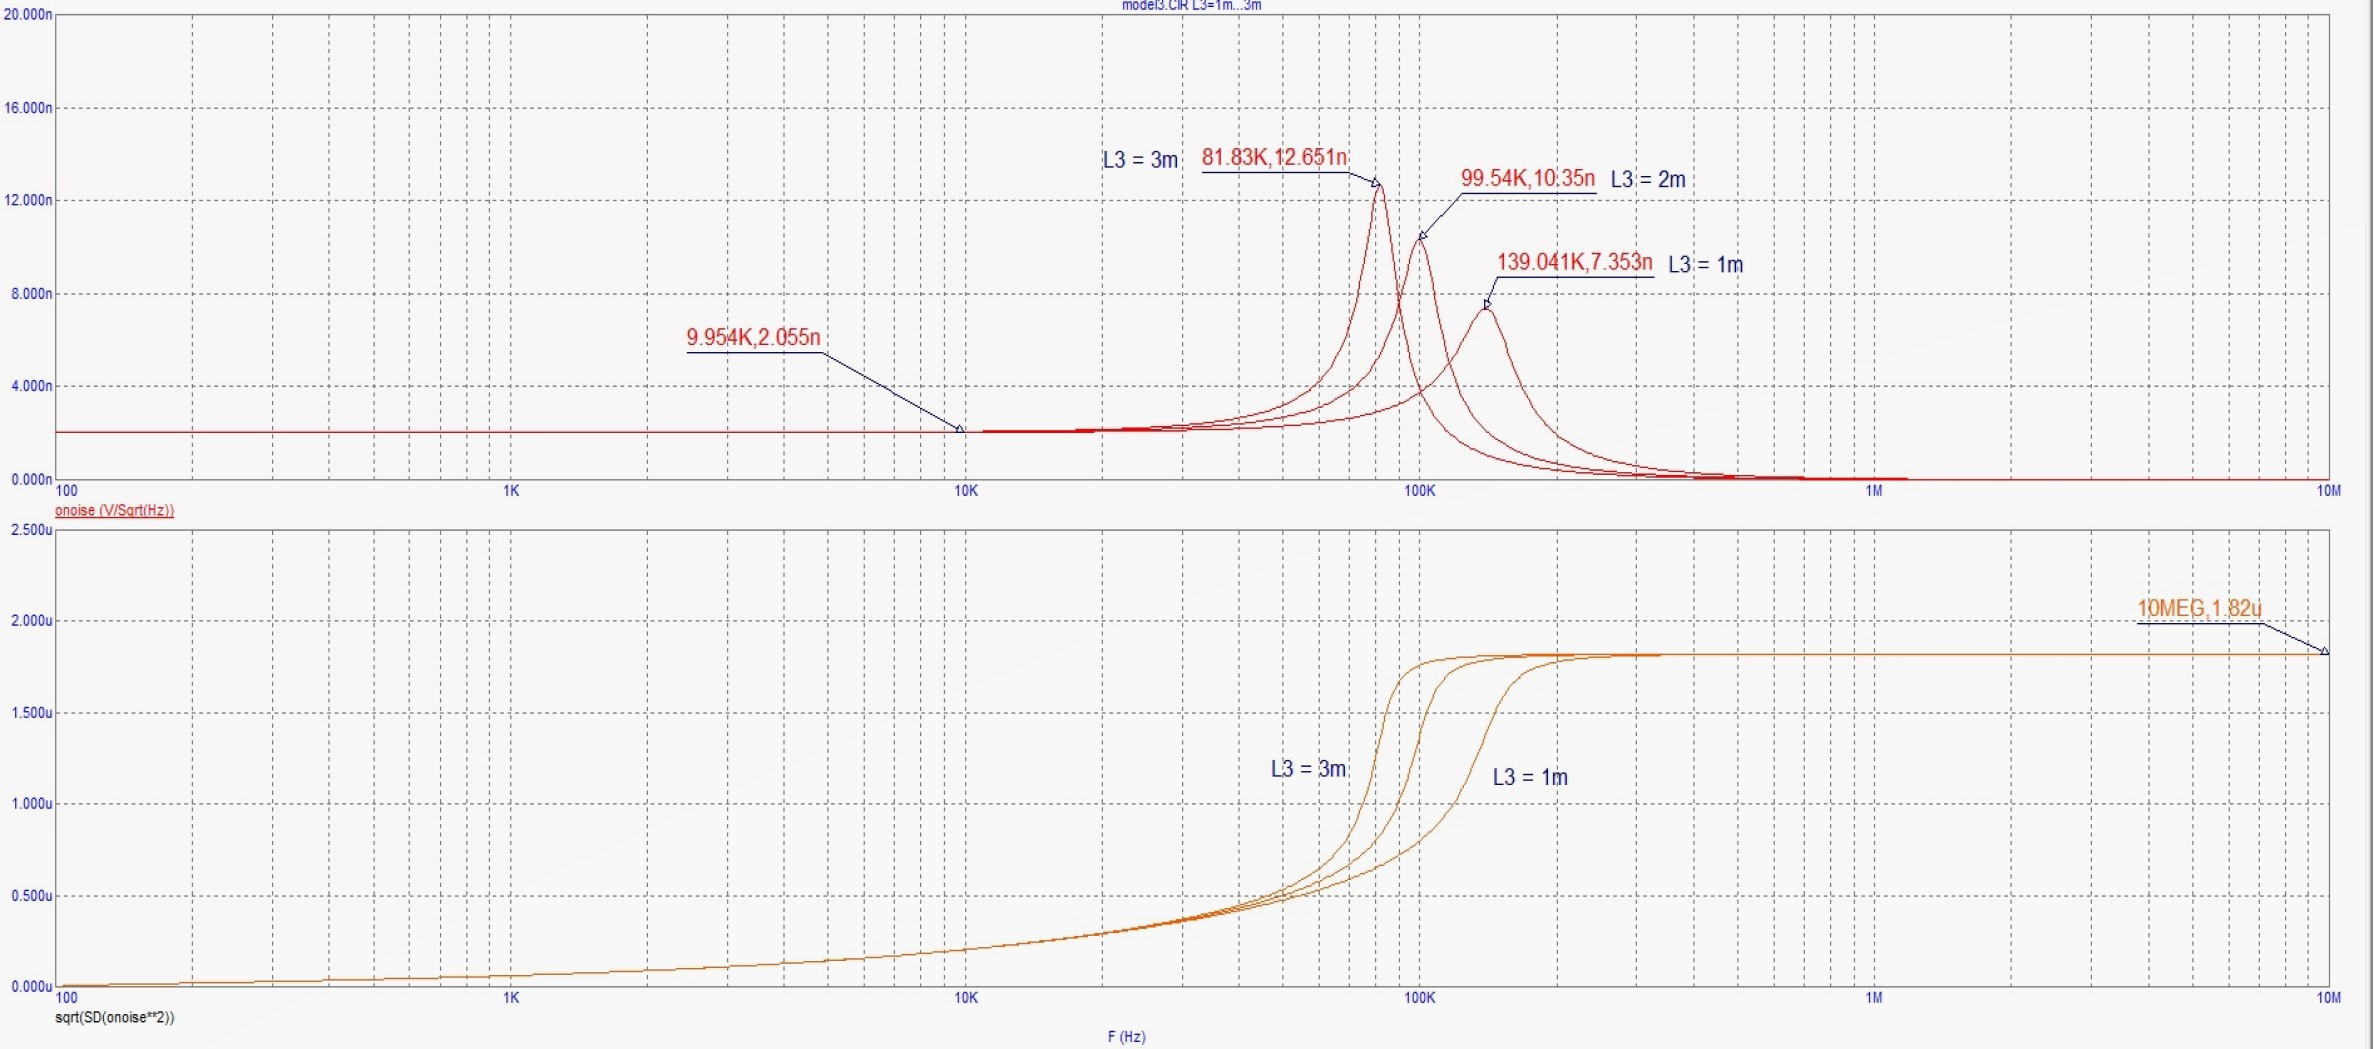
\includegraphics[width=1.1\linewidth]{3/3_3_4.jpg}
			\caption{Задание 3.3, пункт 2, варьирование L}
			\label{A}
\end{figure}

\subsection{Установить $\frac{V4}{n4}$ ($LC$--фильтр верхних частот)}

Рассмотрим LC - фильтр верхних частов с параметрами секции 3.3.


$ \textbf{1.} $


Измерим шумовое напряжение $n_4$ в максимуме при $f_0$ и на частоте $10f_0$, уровень шума $\sigma$ на выходе в полосе $1MHz$.

1) $f_0 = 99.54K \Rightarrow n_4 = 10.35n $

2) $10f_0 = 990.54k \Rightarrow n_4 = 2.056n$

3) $\sigma = 2.692u$


\begin{figure}[h!]
			\centering
			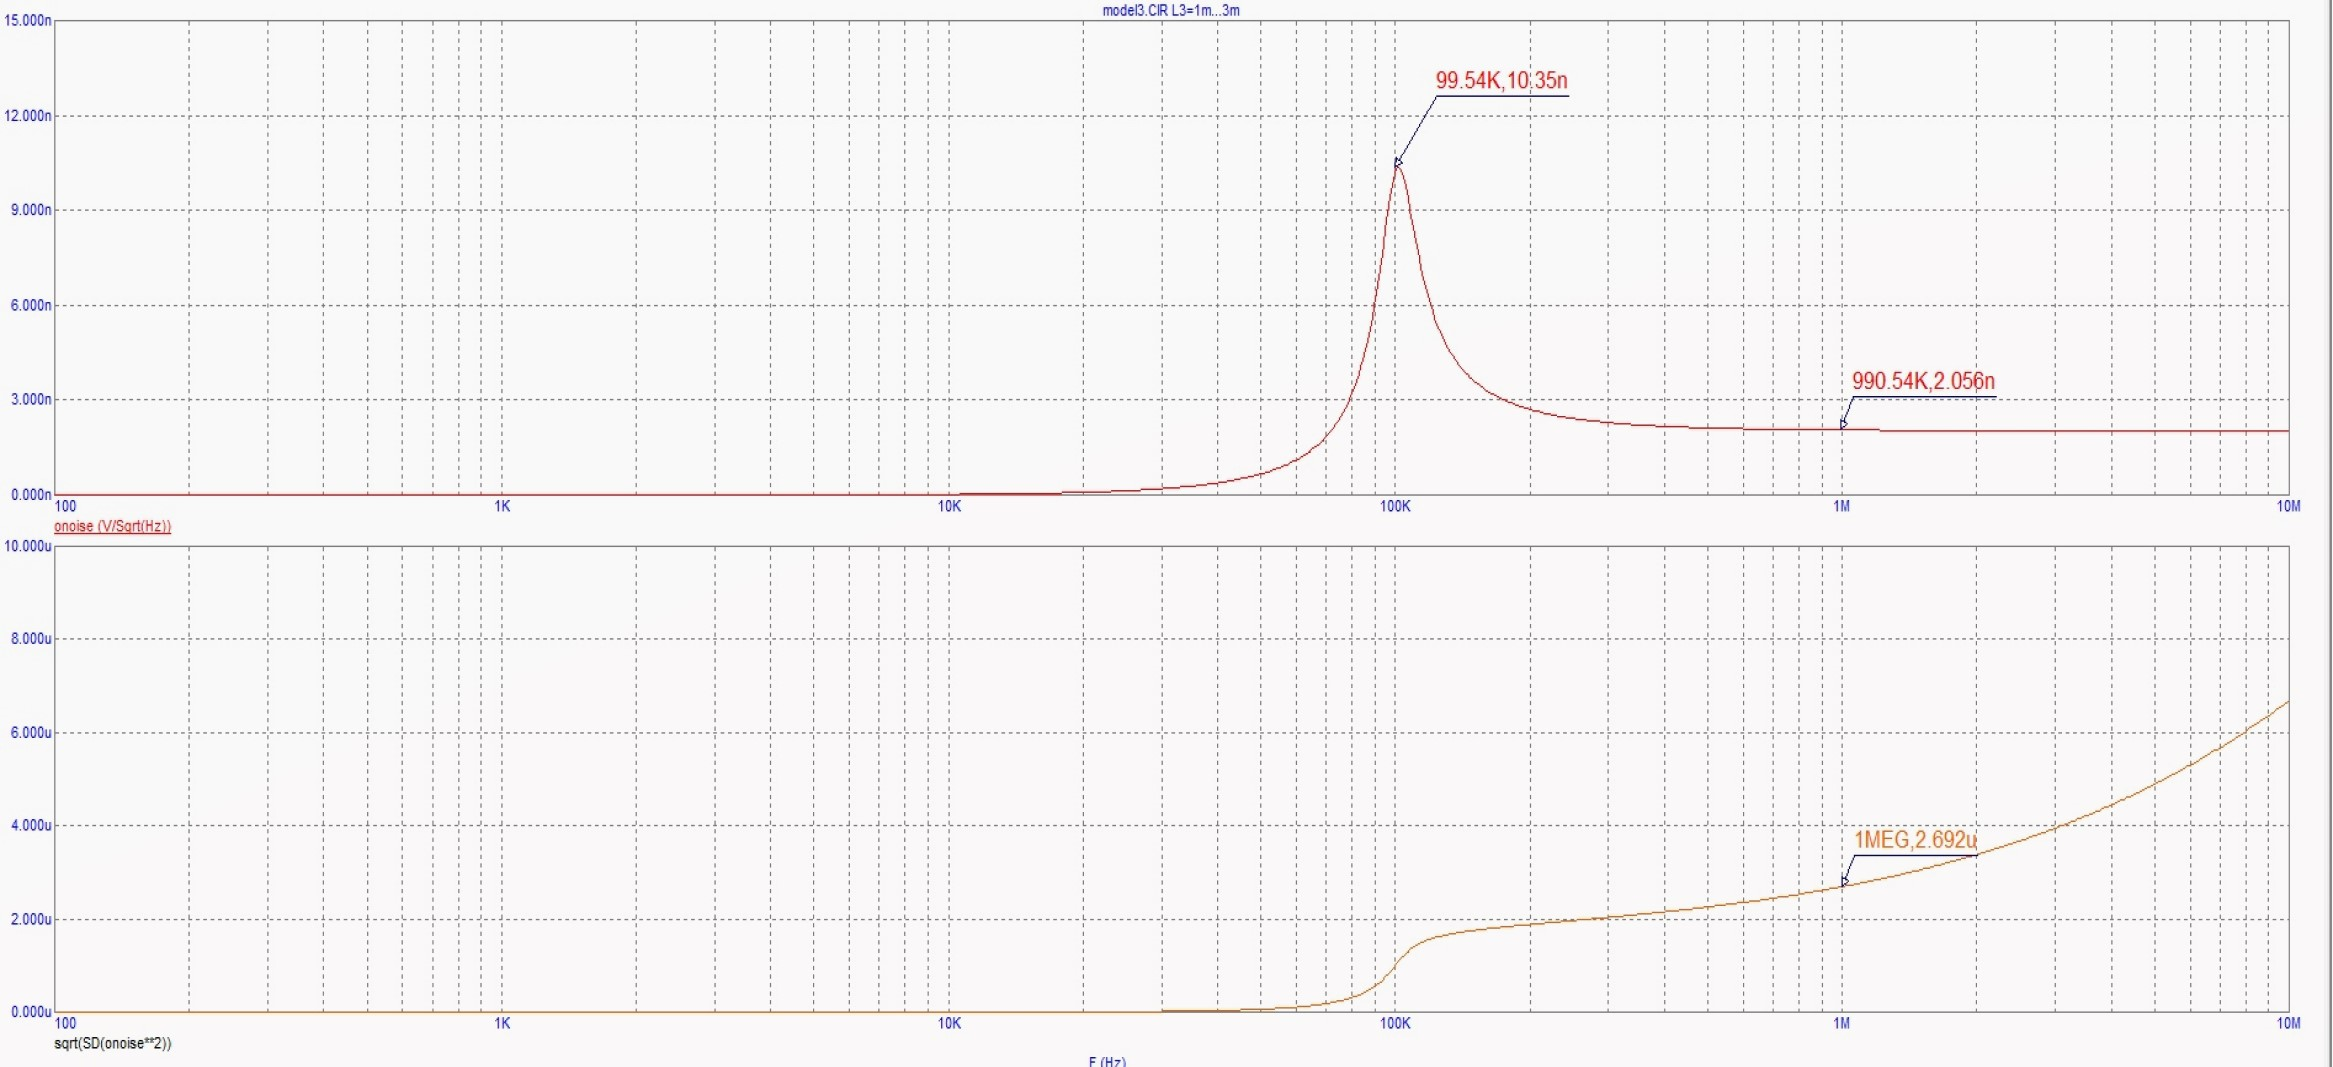
\includegraphics[width=1.1\linewidth]{3/3_3_6.jpg}
			\caption{Задание 3.4, пункт 1}
			\label{A}
\end{figure}

$ \textbf{2.} $

Варьирование $R_4[100, 400 | 150]$.

Варьирование $C_4[0.75n, 1.75n | 0.5n]$.

Варьирование $L_4[1m, 3m | 1m]$.

Фиксируем зависимости $n_4(f_0), \: n_4(10f_0), \: \sigma$ от изменяемых параметров.

\begin{figure}[h!]
			\centering
			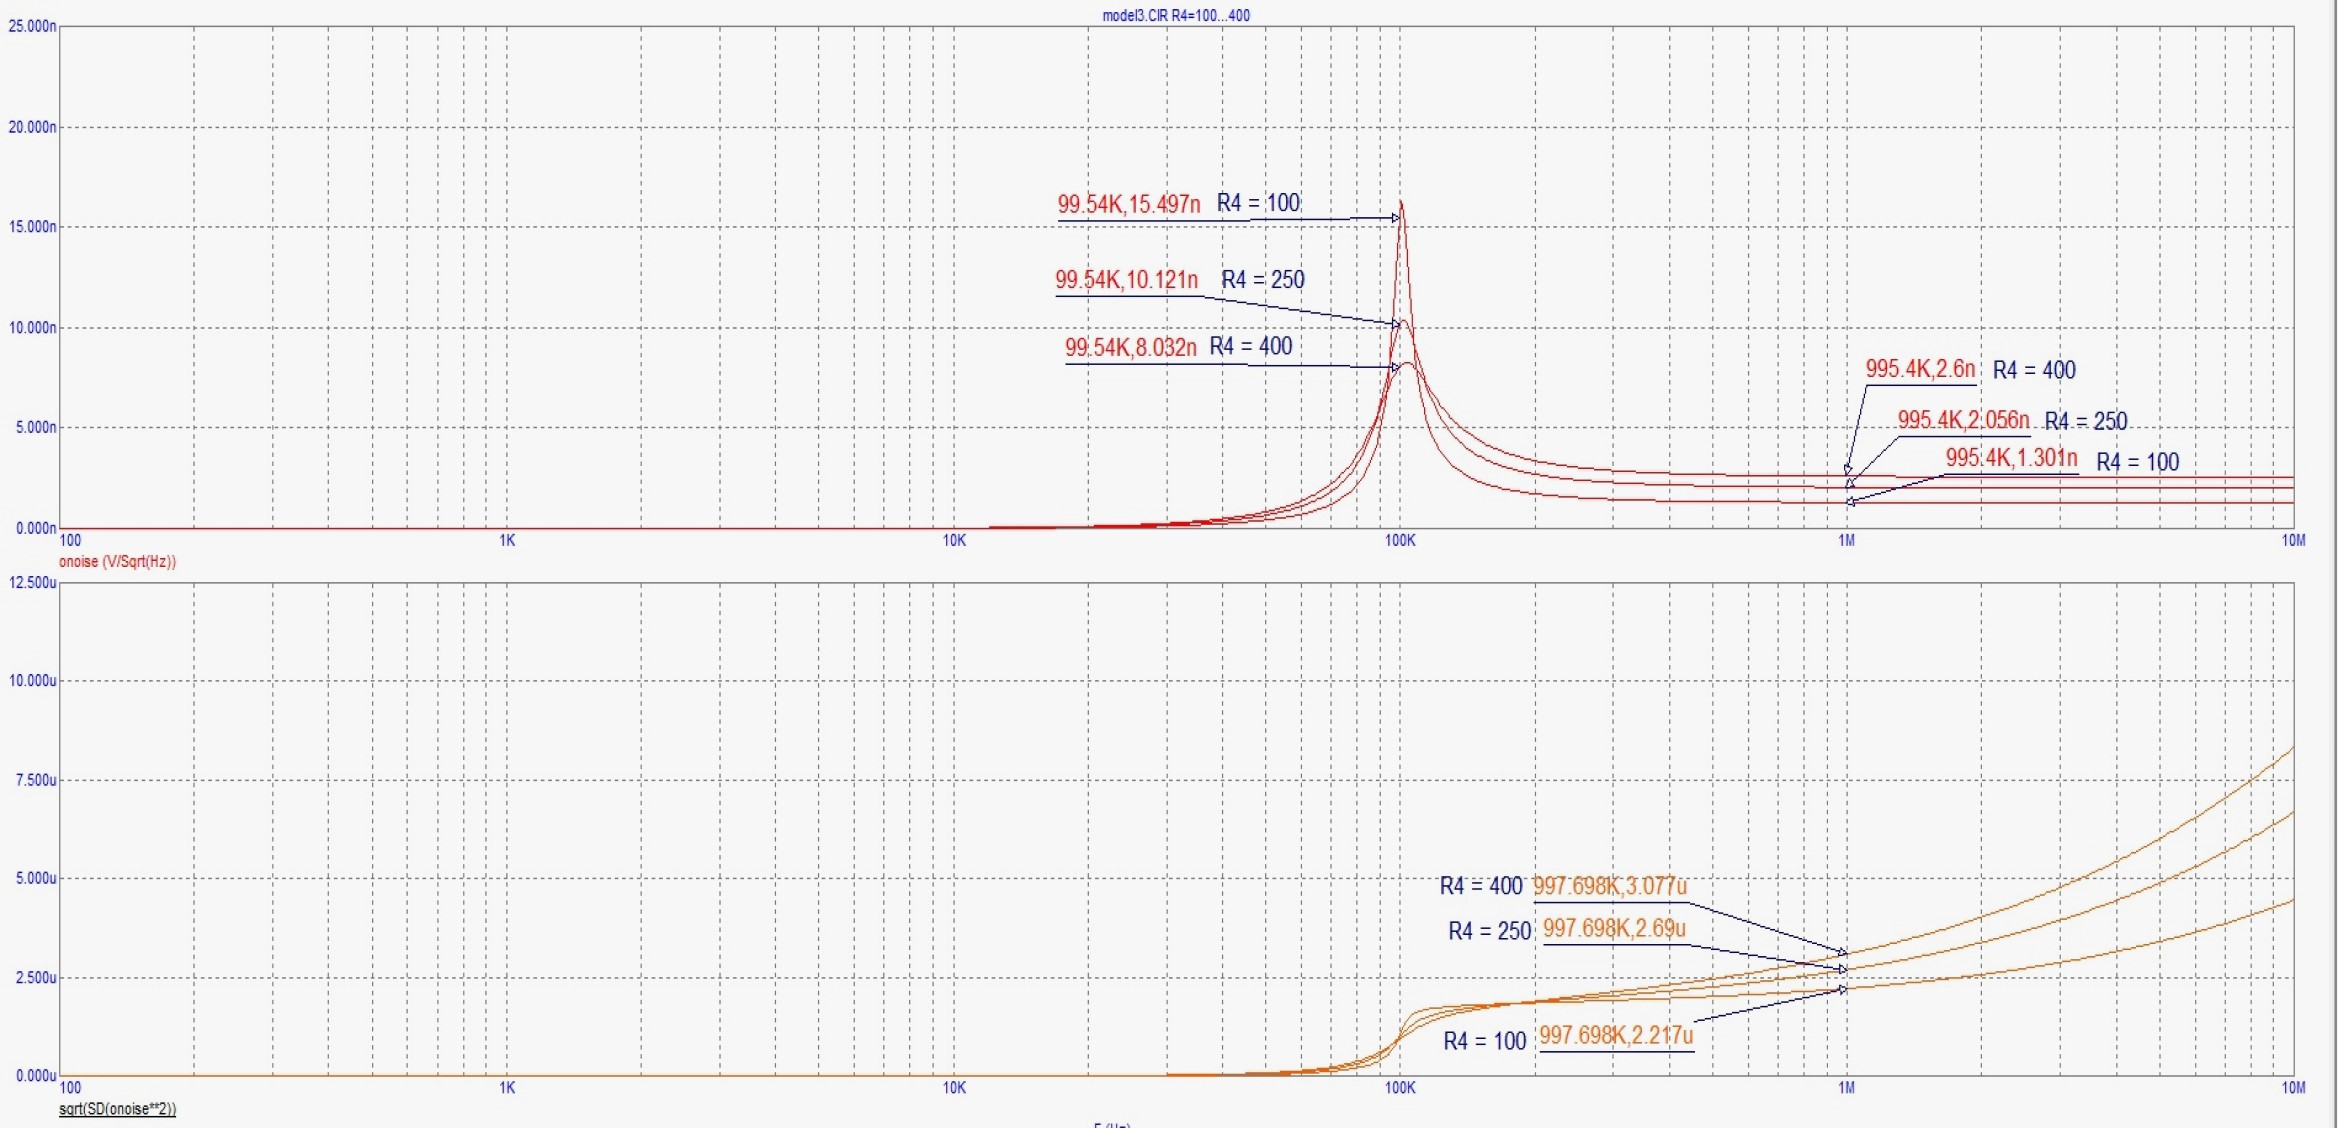
\includegraphics[width=1.1\linewidth]{3/3_4_3.jpg}
			\caption{Задание 3.4, пункт 2, варьирование R}
			\label{A}
\end{figure}


\begin{figure}[h!]
			\centering
			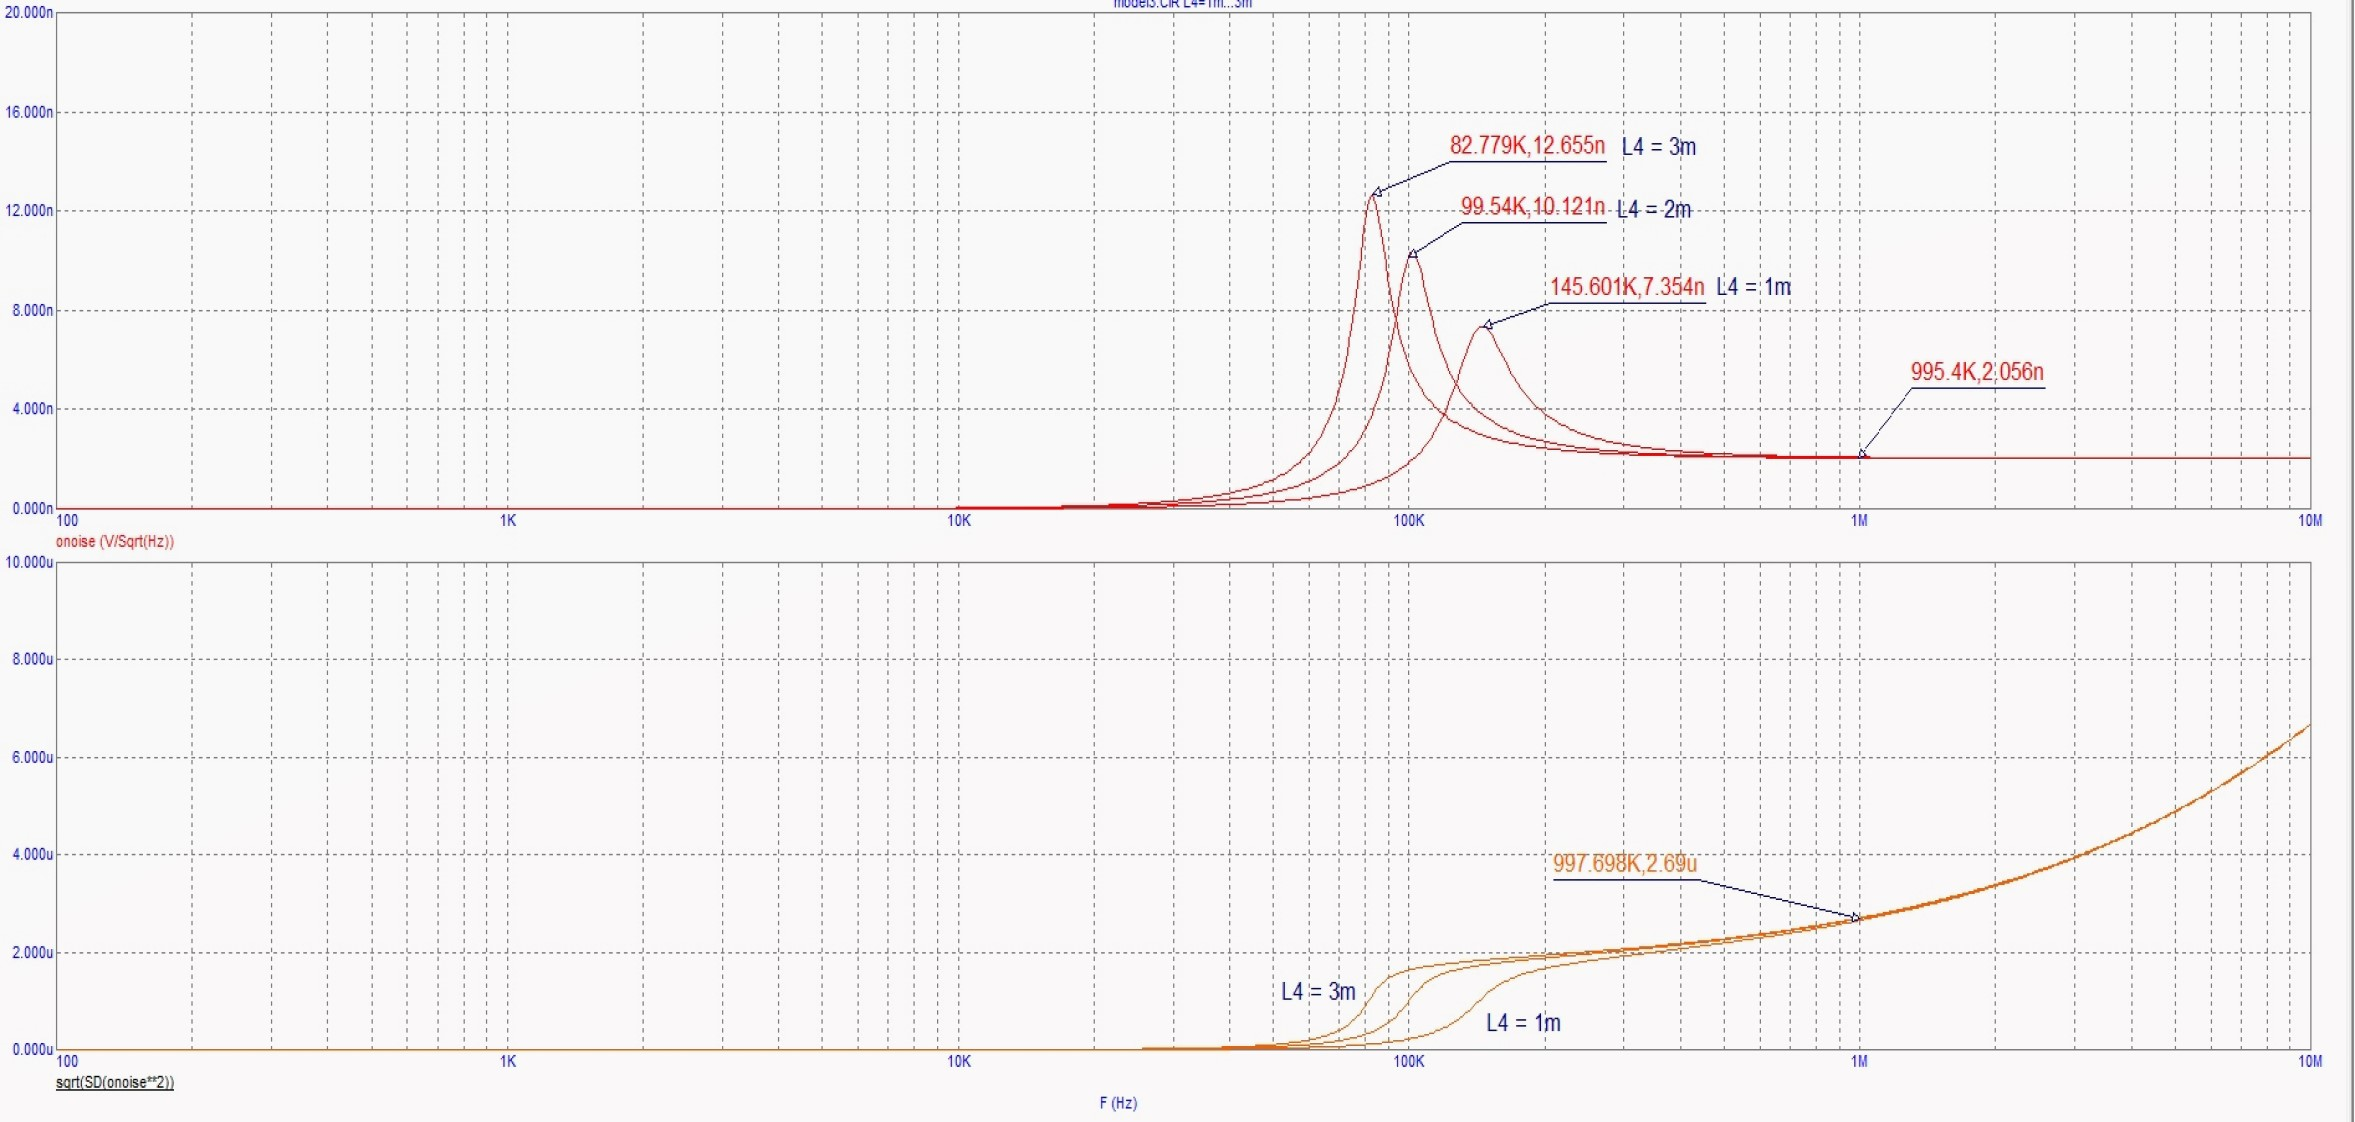
\includegraphics[width=1.1\linewidth]{3/3_4_2.jpg}
			\caption{Задание 3.4, пункт 2, варьирование С}
			\label{A}
\end{figure}


\begin{figure}[h!]
			\centering
			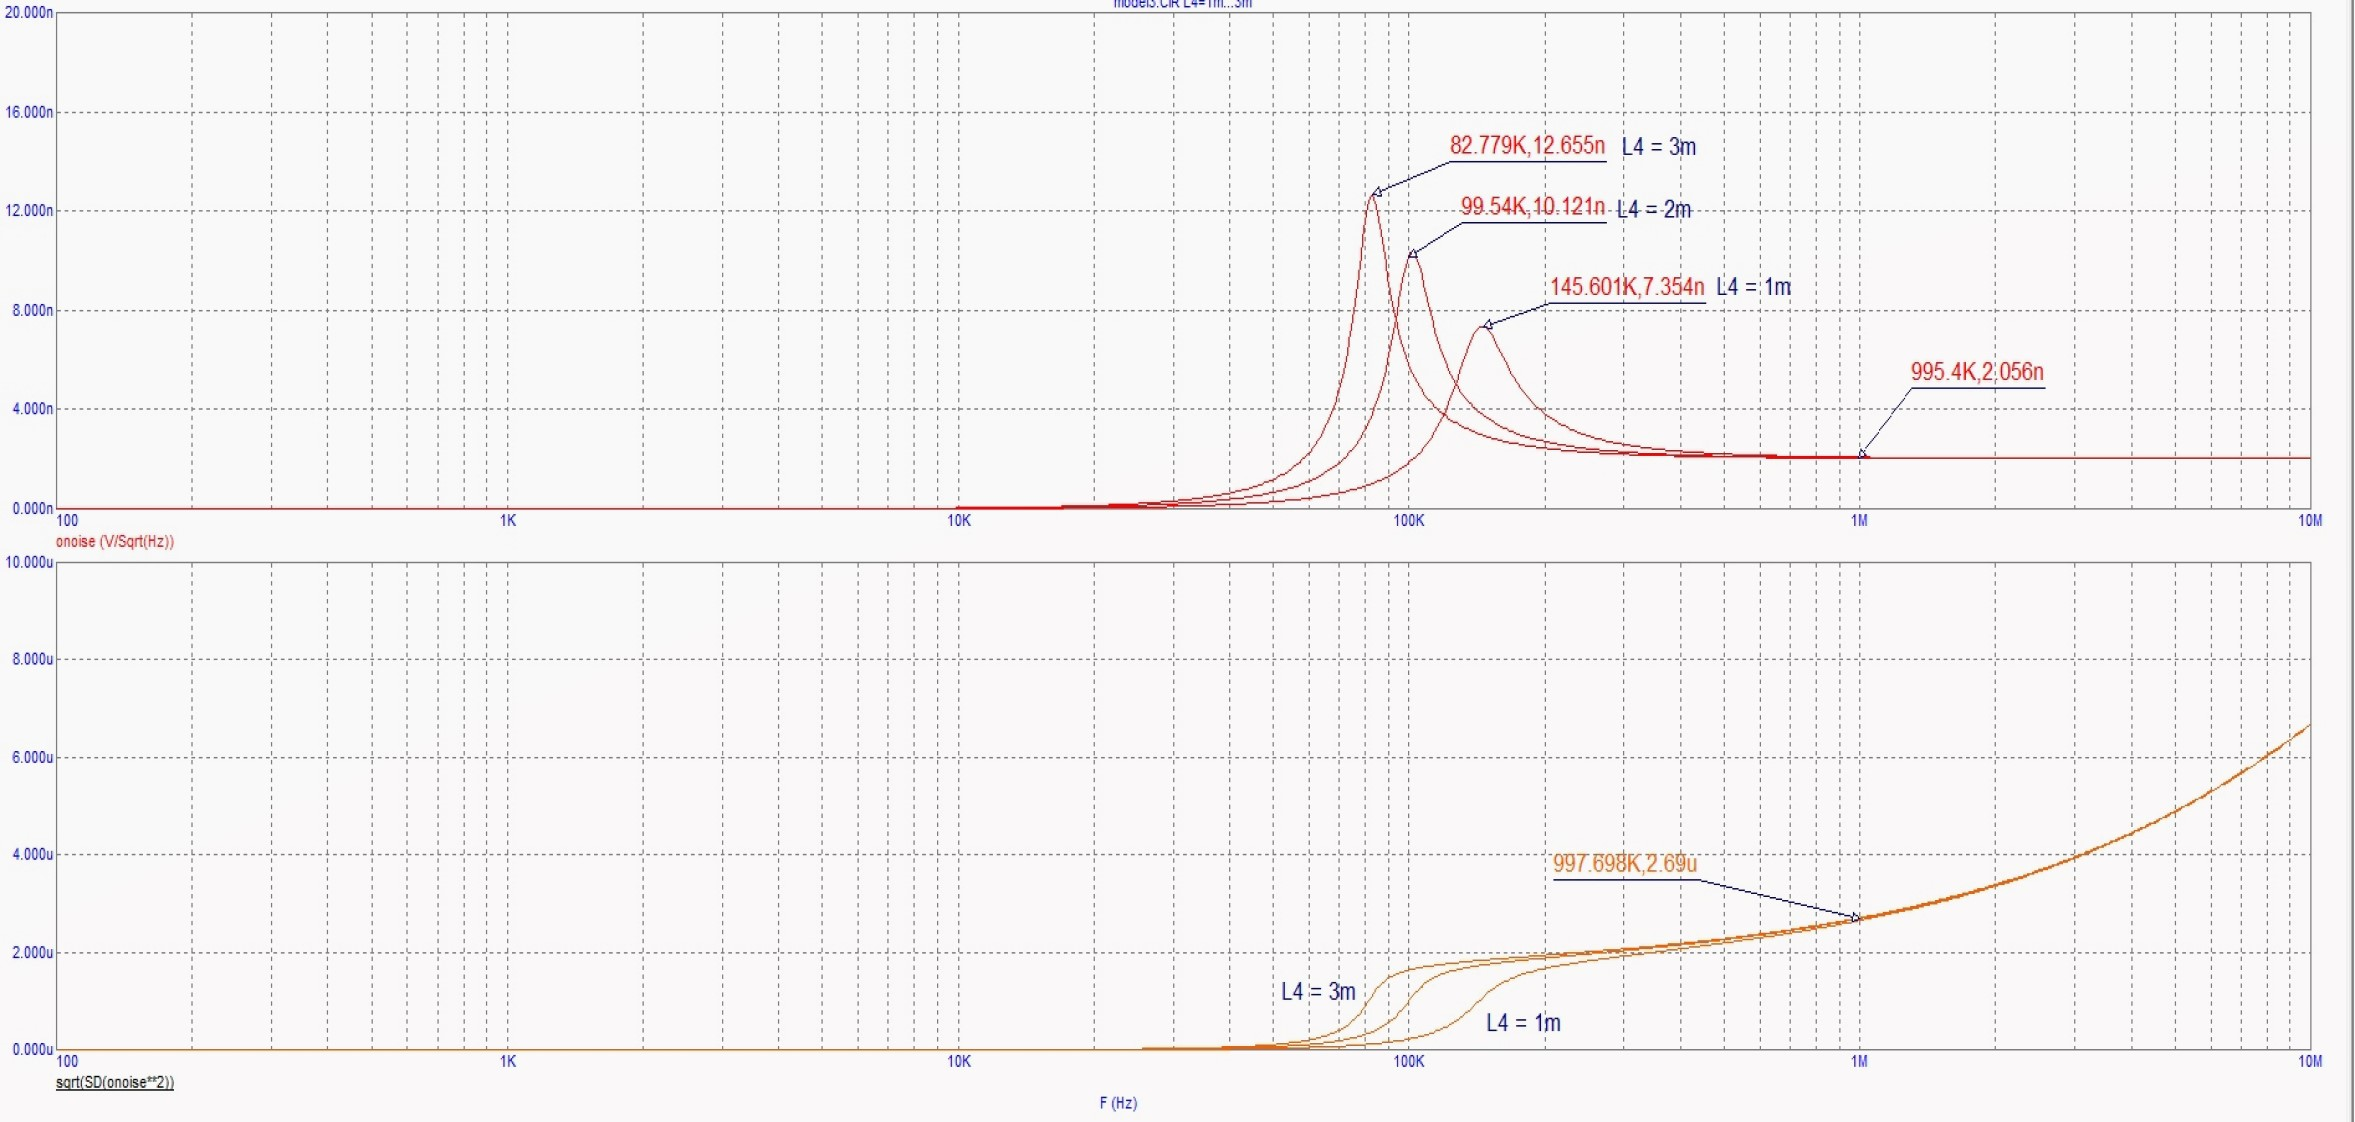
\includegraphics[width=1.1\linewidth]{3/3_4_2.jpg}
			\caption{Задание 3.4, пункт 2, варьирование L}
			\label{A}
\end{figure}




\newpage

\section{Шумящие фильтры}

\subsection{Полосовой $LC$--фильтр}

$ $

$\textbf{1.} $

Открыаем файл model4.
Установим $\{n1/V1\}$ : фильтр 1 с параметрами:


\[ f_0 = 100kHz, \rho = 1260, Q = 3\]


Подключив $v(n_1)/(v(V1)$ снимем АЧХ фильтра. Измерим резонансную частоту $f_0$, полосу по уровню 0.7, коэффициент передачи на резонансной и нулоевой частотах.

Сравним с теорией.

1) $f_0 = 100k, \Delta f = 35k$.

2) По графику:$K{f_0} \approx 0.5$.

3) Теоретический расчет по формуле:

\[ K = \frac{0.5}{1 + jQ\cdot(\frac{f}{f_0} - \frac{f_0}{f})}\]

Получаем, что $K_1 = 0.5$.

С теорией совпало.

\begin{figure}[h!]
			\centering
			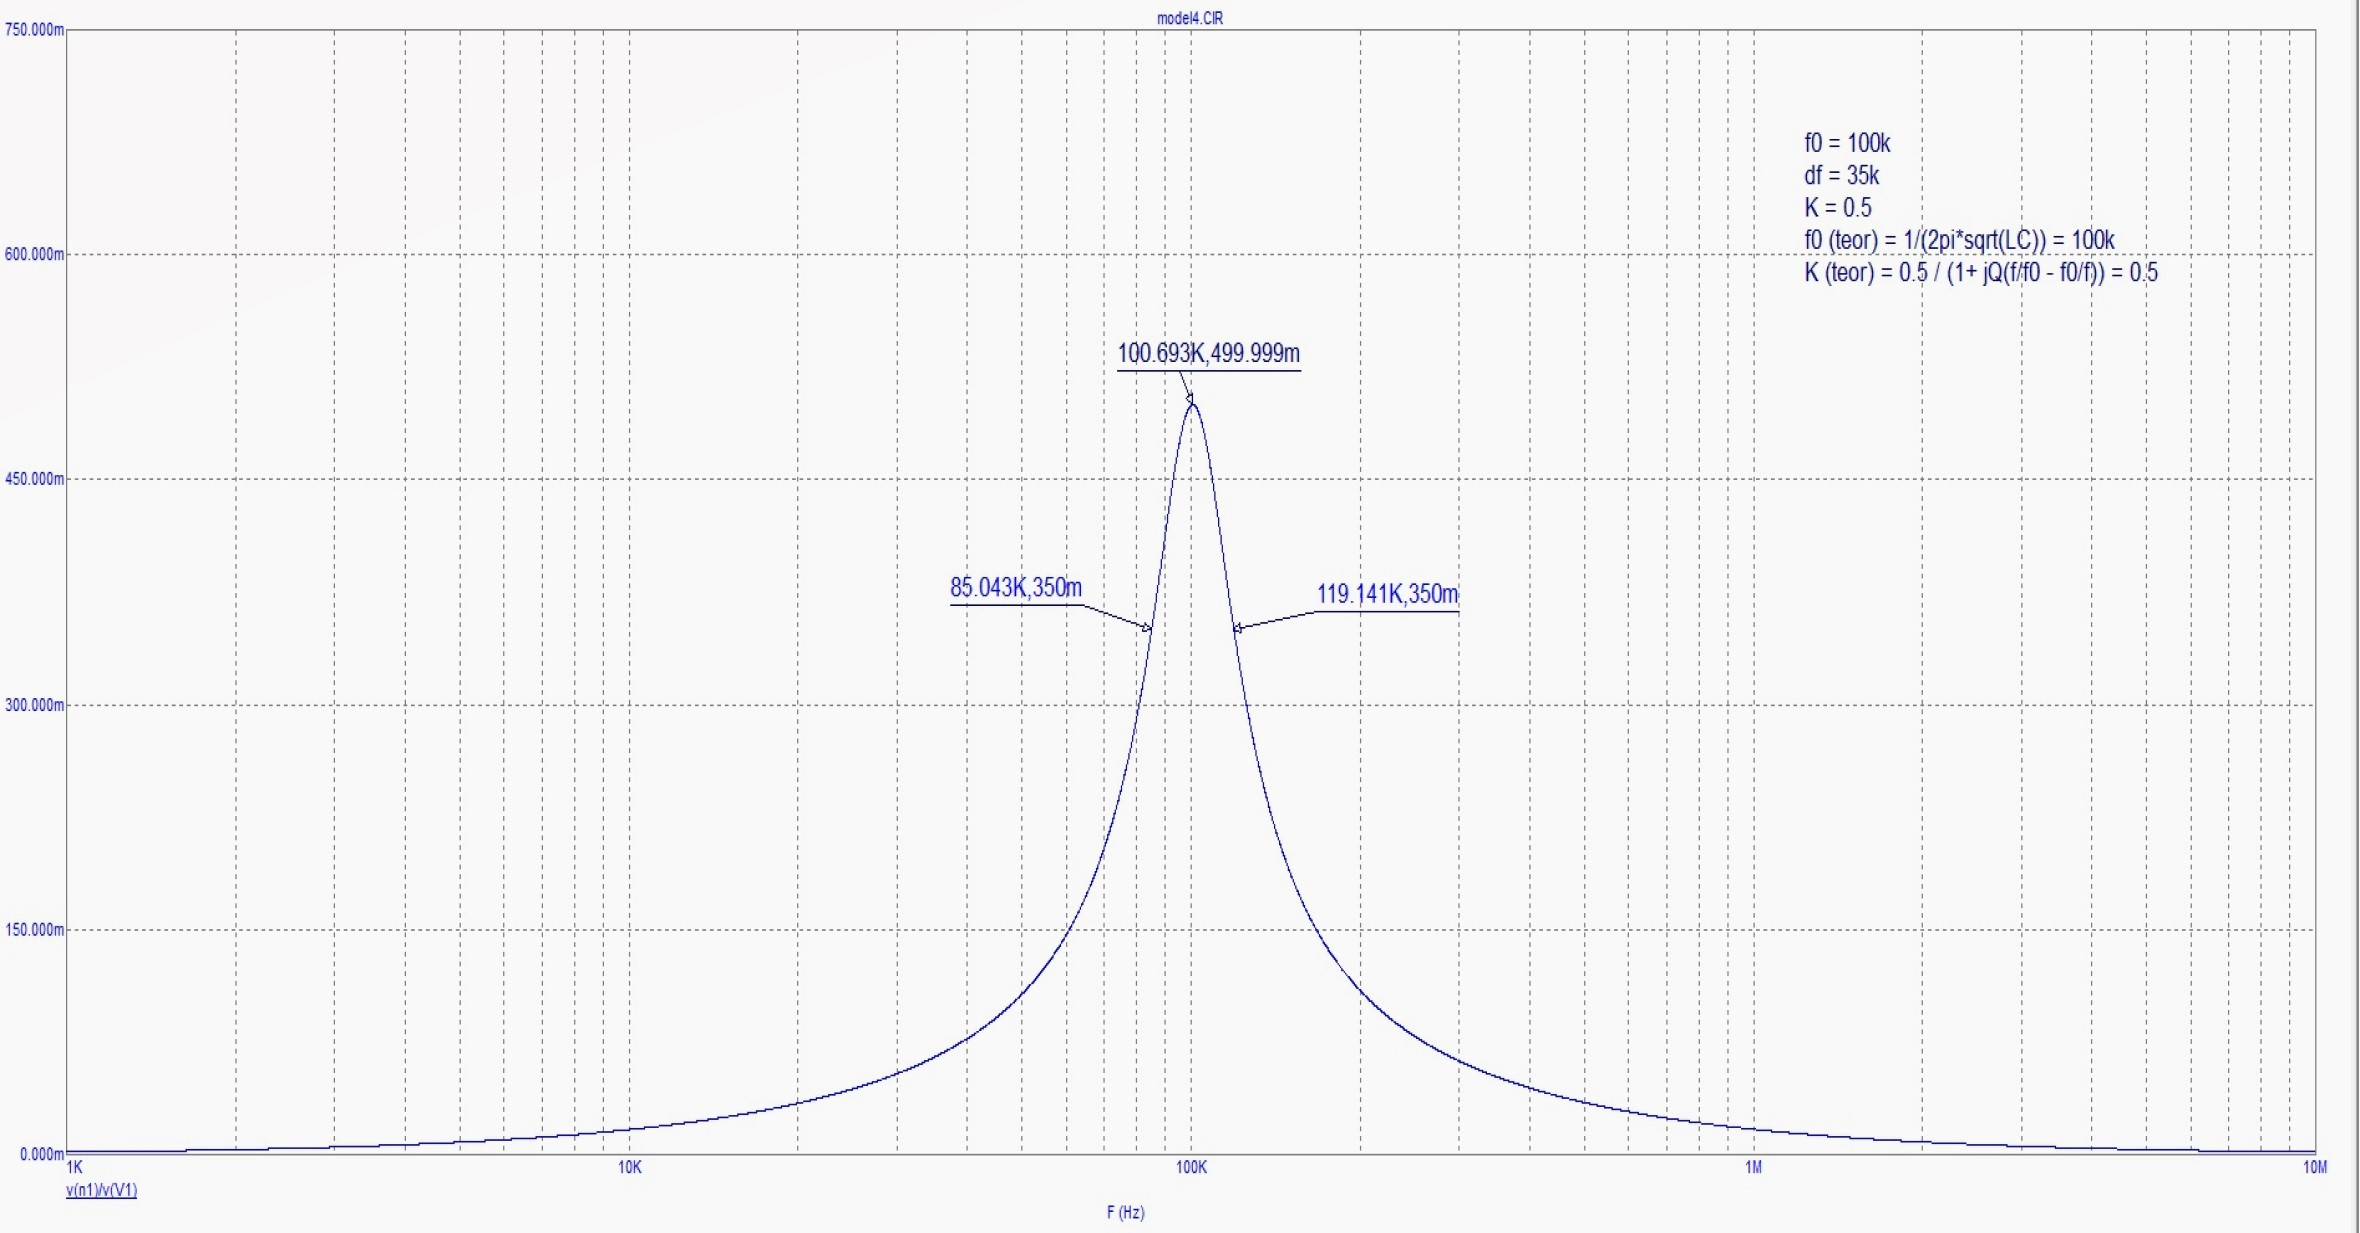
\includegraphics[width=1.1\linewidth]{4/4_1_2.jpg}
			\caption{Задание 4.1, пункт 1}
			\label{A}
\end{figure}


$\textbf{2.} $



Измерим уровни шумвого напряжения на частотах $f_0, f_0/10$. Так же заменим поочередно первый и второй резисторы нешумящим сопротивлением $H_1$, оценим вклад шумов $R_{s1}, R_1$ в шумовое напряжение и в уровень шума на выходе:
1) $n_{f_0} = 1.32n, \: n_{\frac{f_0}{10}} = 1.865n, \: \sigma = 1.819u$

2) $n_{f_0} = 994p, \: n_{\frac{f_0}{10}} = 1.865p, \: \sigma = 5.88u$

3) $n_{f_0} = 994.8p, \: n_{\frac{f_0}{10}} = 35p, \: \sigma = 235n$

\begin{figure}[h!]
			\centering
			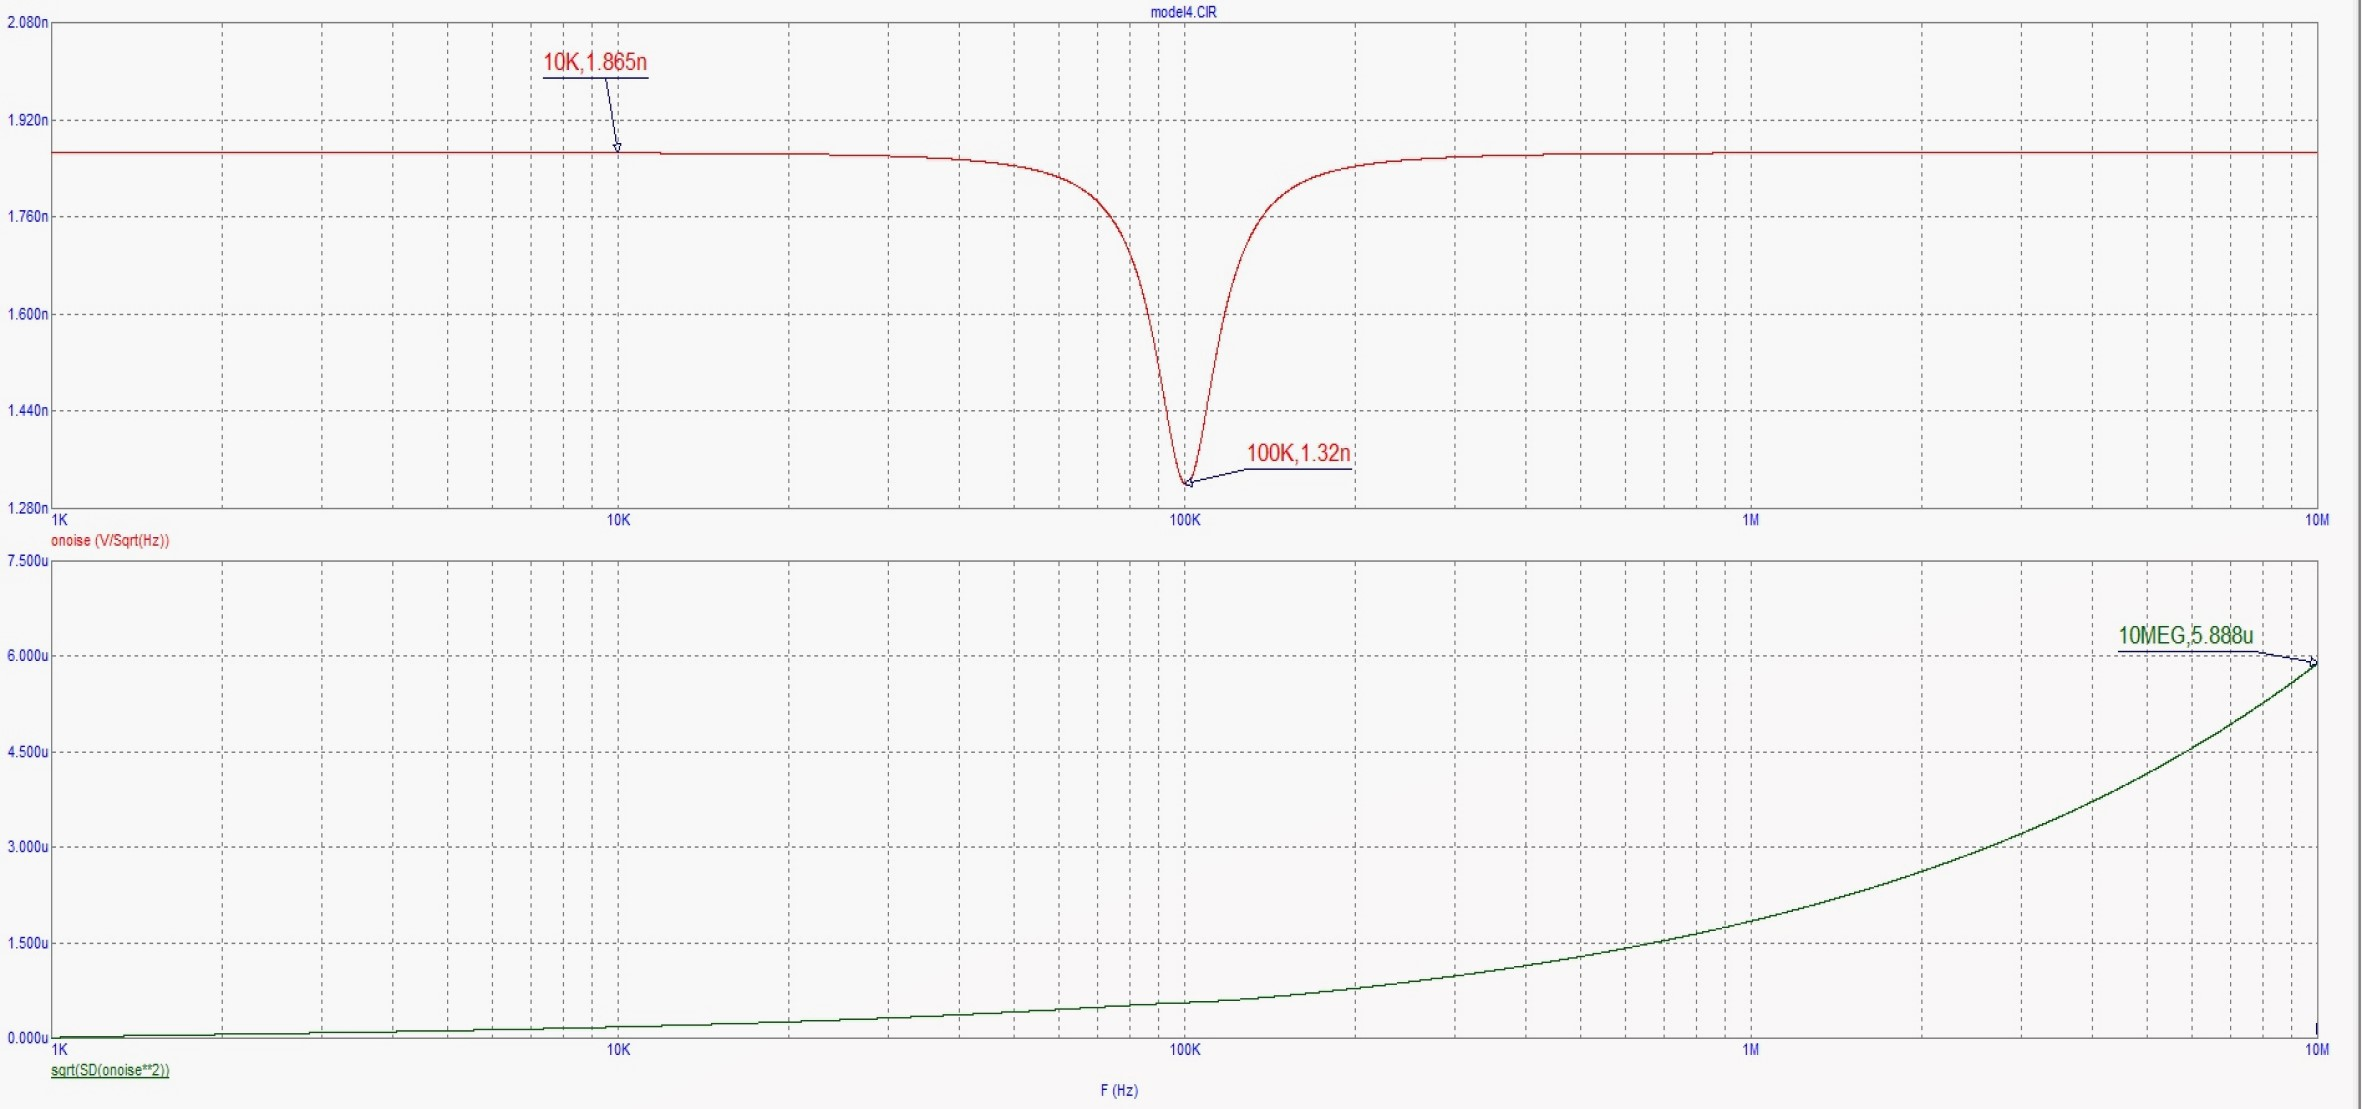
\includegraphics[width=1.1\linewidth]{4/4_1_3.jpg}
			\caption{Задание 4.1, пункт 2}
			\label{A}
\end{figure}




\begin{figure}[h!]
			\centering
			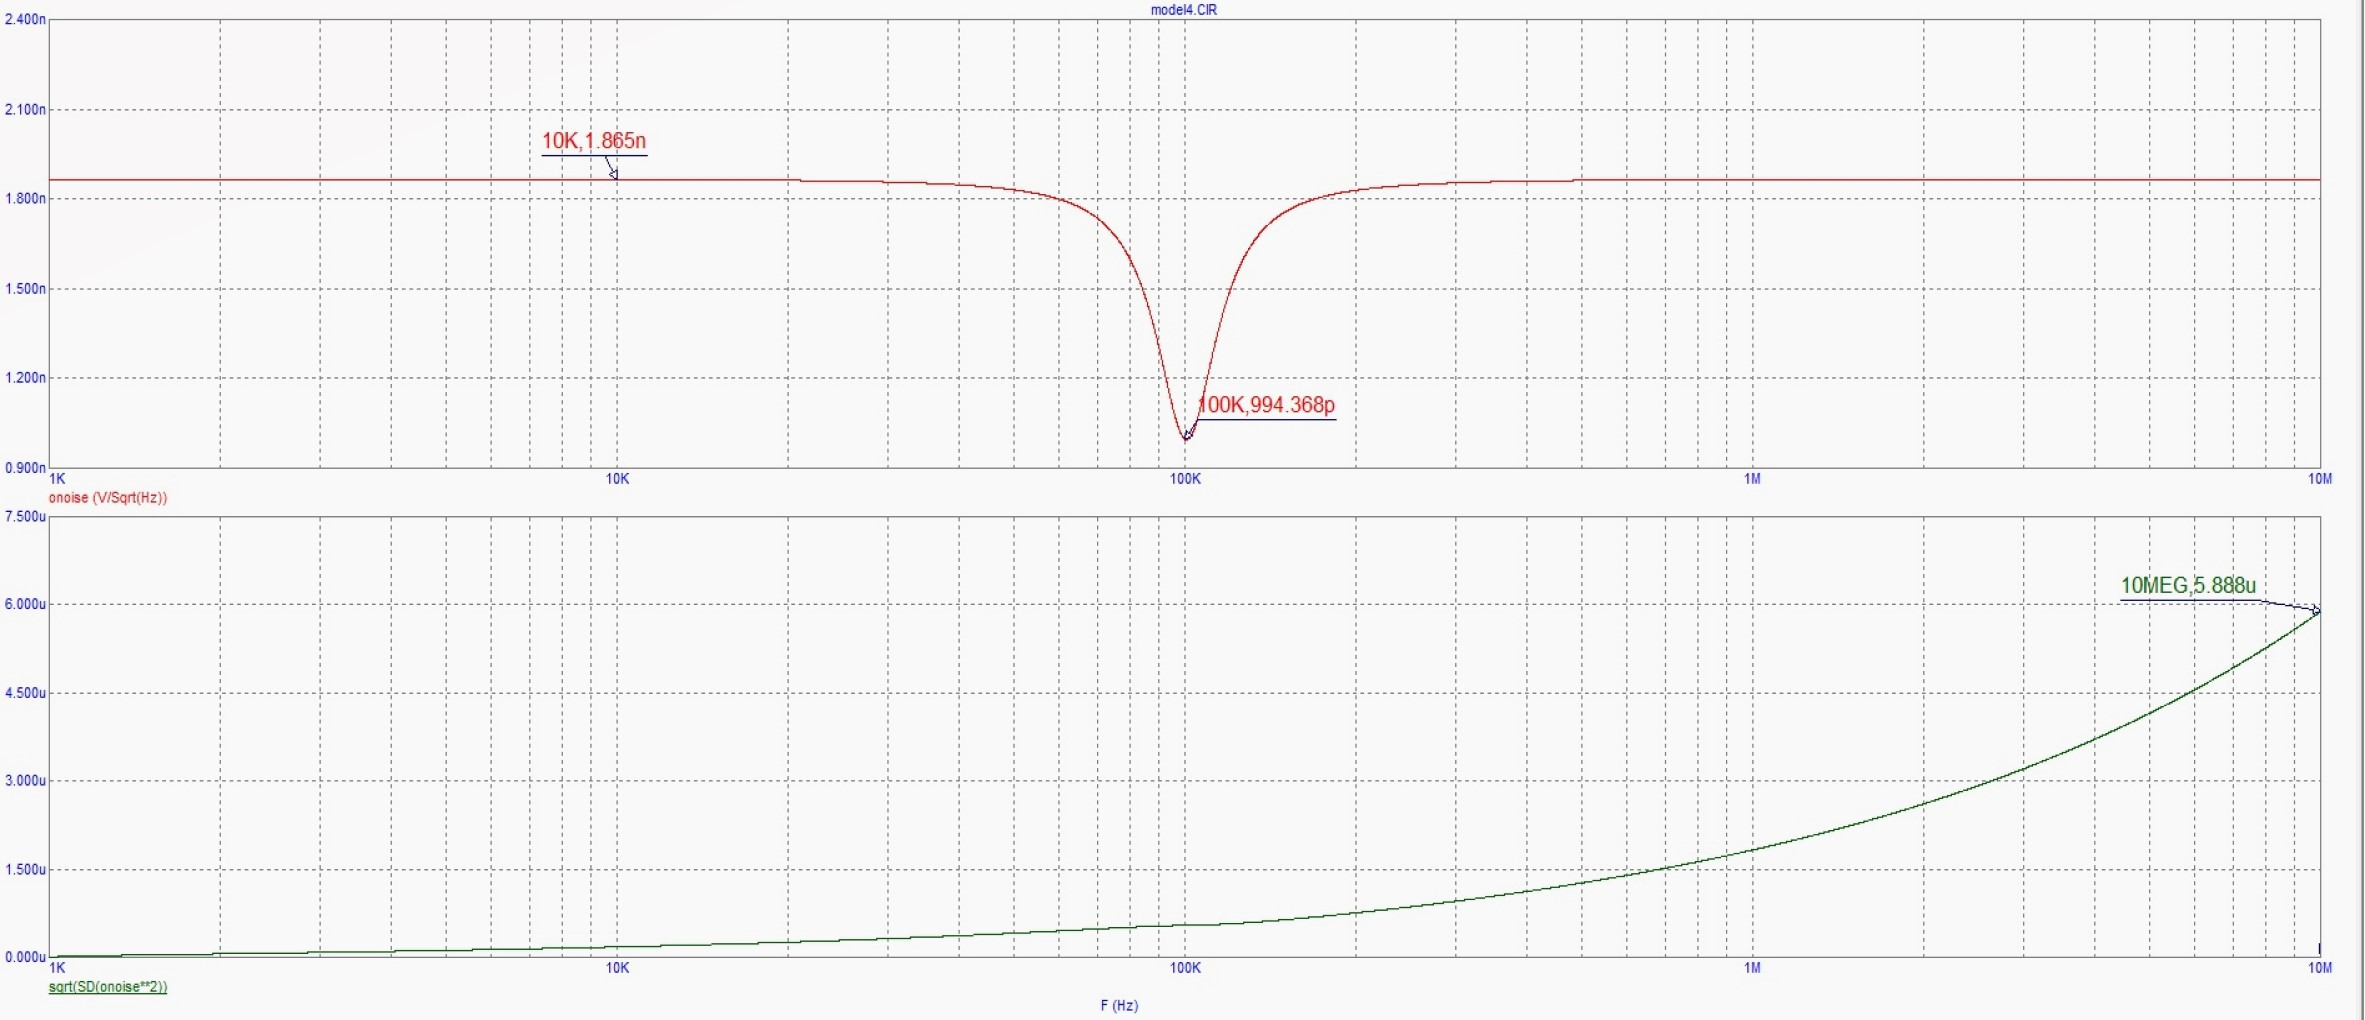
\includegraphics[width=1.1\linewidth]{4/4_1_5.jpg}
			\caption{Задание 4.1, пункт 2}
			\label{A}
\end{figure}



\begin{figure}[h!]
			\centering
			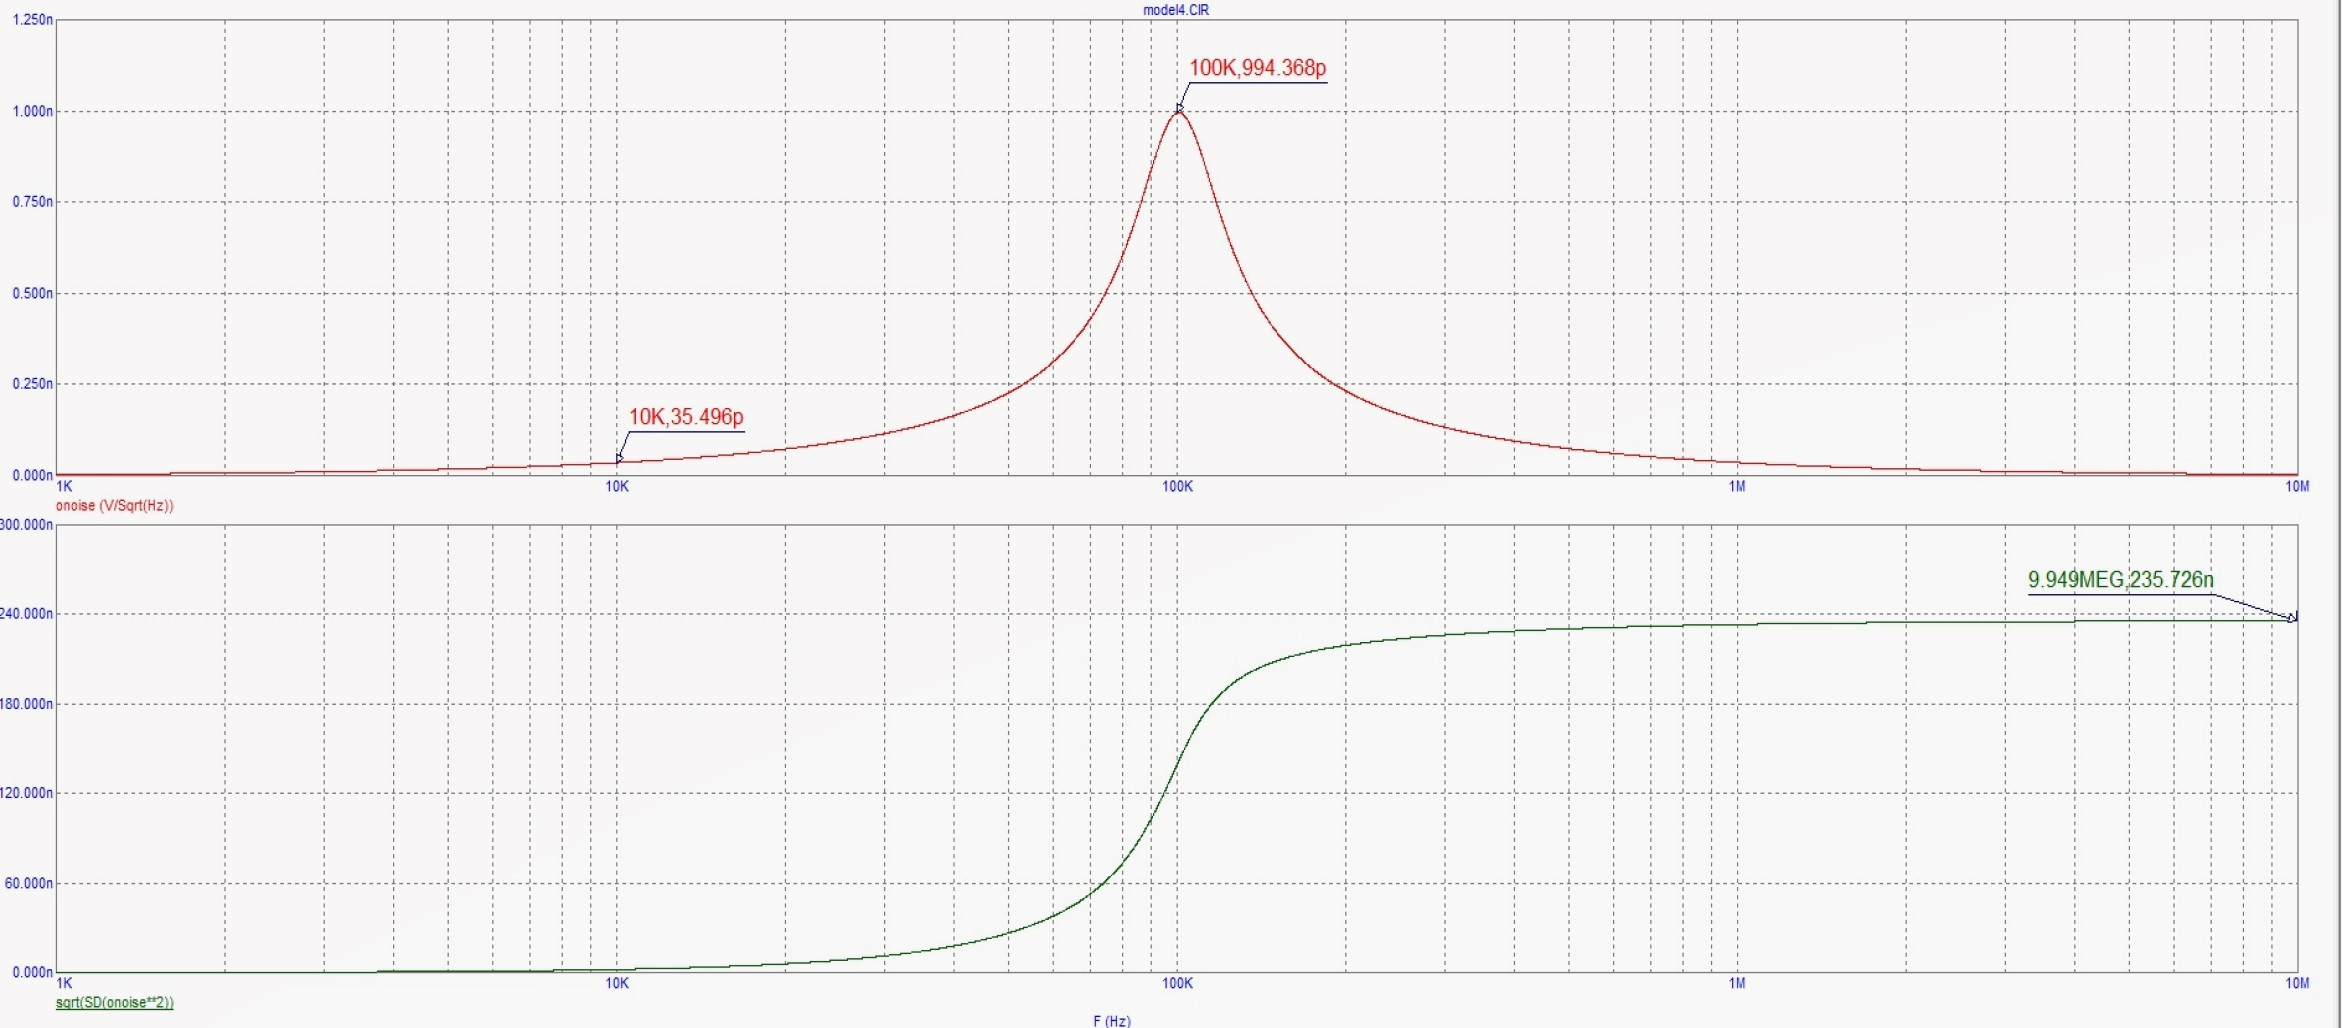
\includegraphics[width=1.1\linewidth]{4/4_1_4.jpg}
			\caption{Задание 4.1, пункт 2}
			\label{A}
\end{figure}


$\textbf{3.} $




По графику рис.36 оцениваем значение коэффициента шума на частотах $f_0$, \:, \: $f_0/10$ по формуле


\[  K_n = 20lg(\frac{e_n(f)}{\sqrt{4kTR}})   \]


1) $e_{f_0}= 112n \Rightarrow K_n(f0) = 3$

2) $e_{f_0/10}= 2.643n \Rightarrow K_n(f_0/10) = 35.6 $



\begin{figure}[h!]
			\centering
			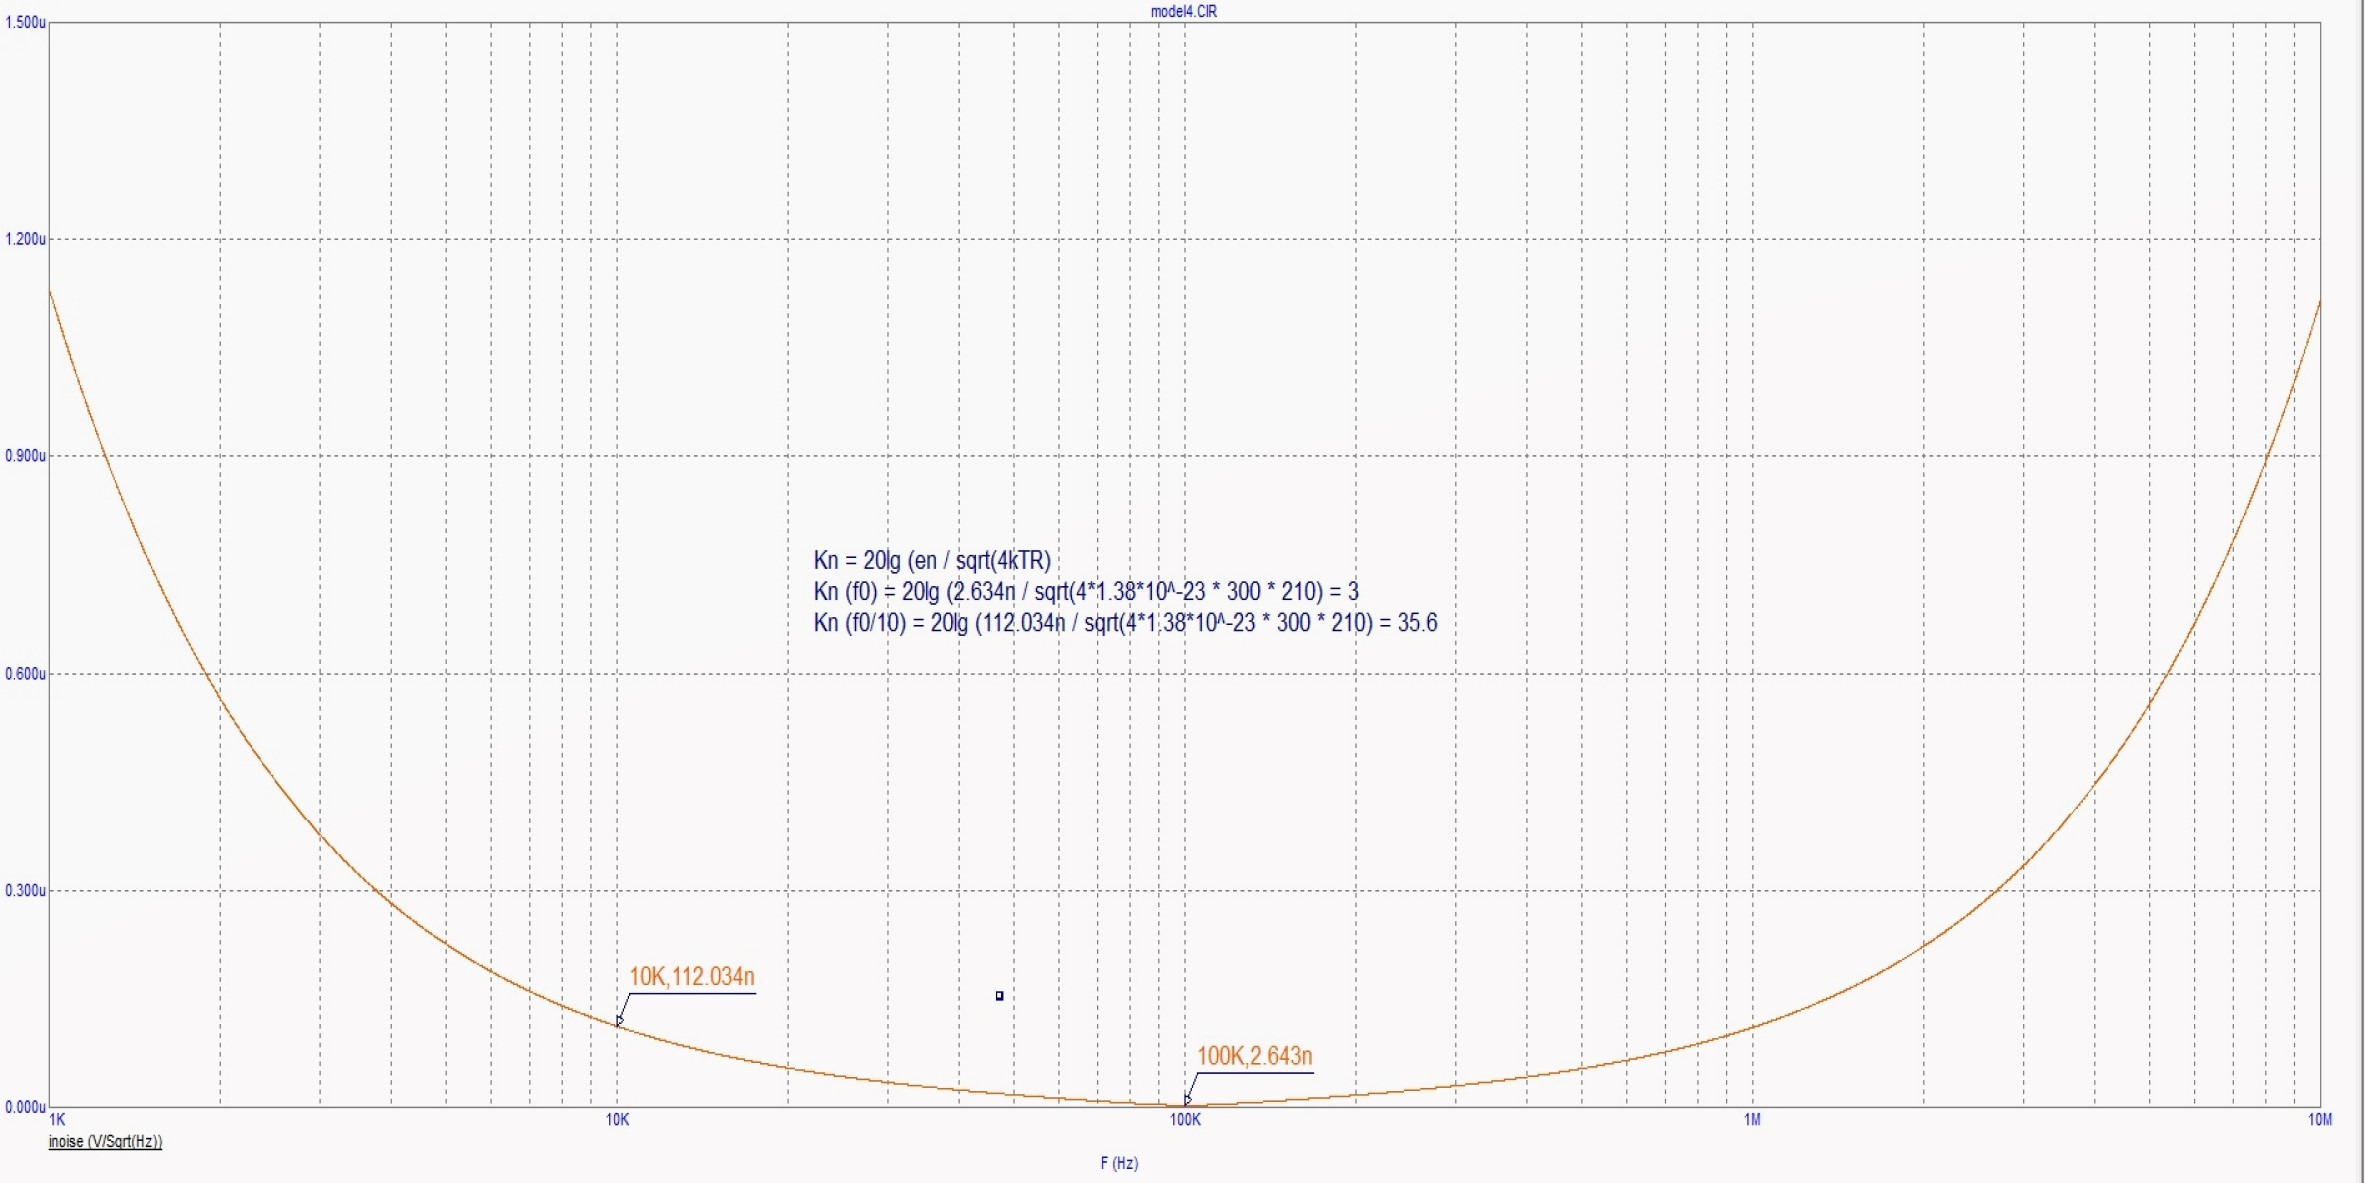
\includegraphics[width=1.1\linewidth]{4/4_1_1.jpg}
			\caption{Задание 4.1, пункт 3}
			\label{A}
\end{figure}

\subsection{Полосовой $RC$--фильтр}

$ $

$\textbf{1.} $


Установим $\{n1/V1\}$ : фильтр 2 с $f_0 = 50kHz$.


Подключив $v(n_2)/(v(V_2)$ снимем АЧХ фильтра. Измерим резонансную частоту $f_0$, полосу по уровню 0.7, коэффициент передачи на резонансной и нулоевой частотах.

Сравним с теорией.

1) $f_0 = 50k, \Delta f = 153k$.

2) По графику: $K_{f_0} \approx 1/3$.

3) Теоретический расчет по формуле:

\[ K = \frac{0.5}{1 + jQ\cdot(\frac{f}{f_0} - \frac{f_0}{f})}\]

Получаем, что $K = 0.34$.

С теорией совпало.


\begin{figure}[h!]
			\centering
			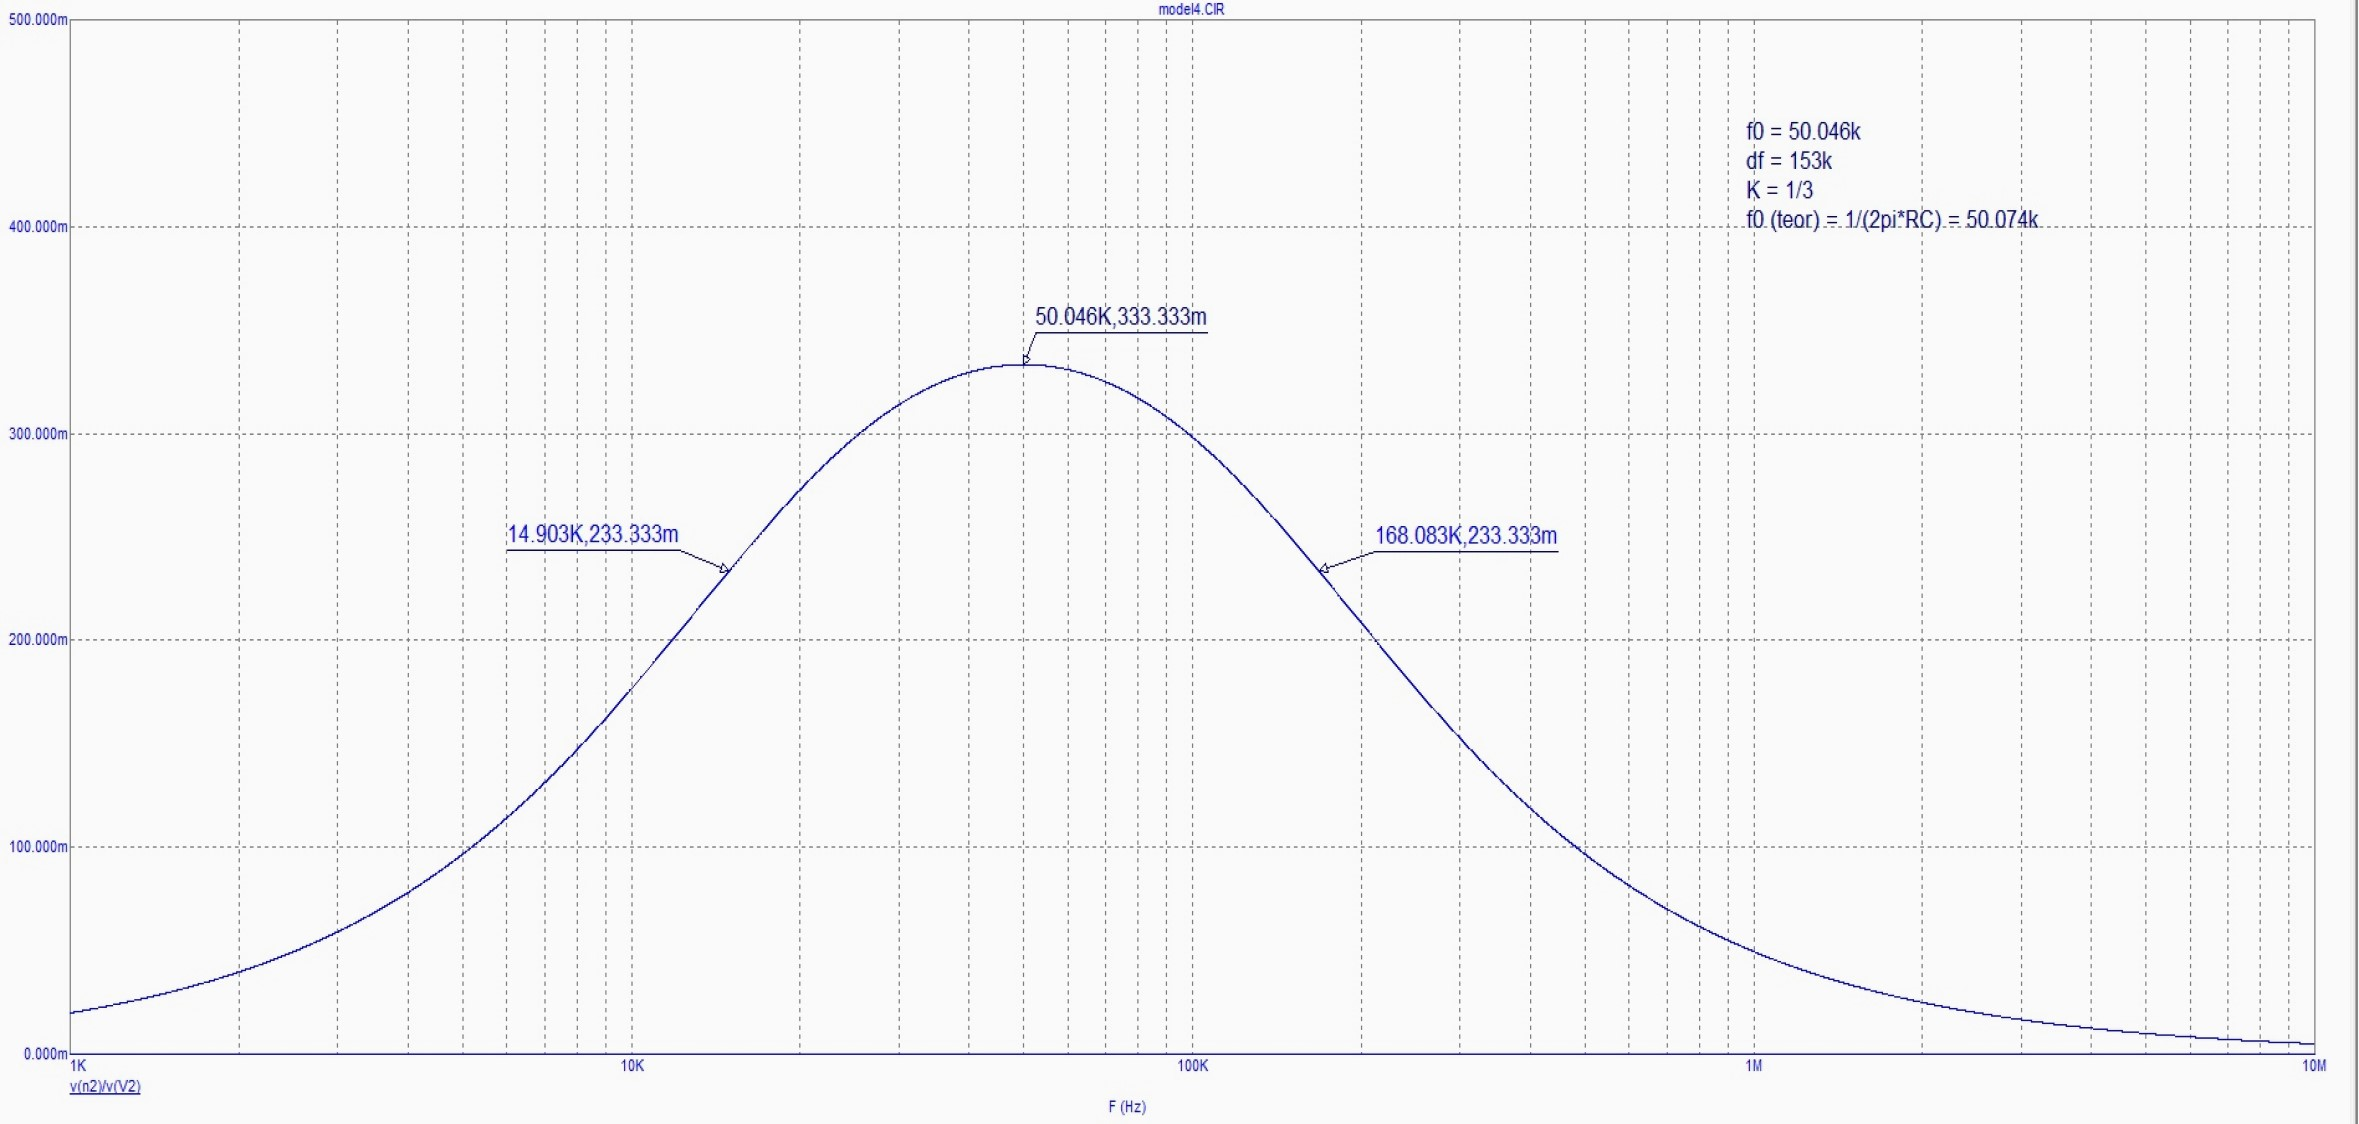
\includegraphics[width=1.1\linewidth]{4/4_2_2.jpg}
			\caption{Задание 4.2, пункт 1}
			\label{A}
\end{figure}


$\textbf{2.} $

Измерим уровни шумвого напряжения на частотах $f_0, \: 10f_0$. Так же заменим поочередно первый и второй резисторы нешумящим сопротивлением $H_1$, оценим вклад шумов $R_{s2}, R_2$ в шумовое напряжение и в уровень шума на выходе:
1) $n_{f_0} = 5.929n, \: n_{10f_0} = 1.572n, \: \sigma = 2.858u$

2) $n_{f_0} = 4.976n, \: n_{10f_0} = 993pp, \: \sigma = 2.141u$

3) $n_{f_0} = 241p, \: n_{10f_0} = 251p, \: \sigma = 370n$


\begin{figure}[h!]
			\centering
			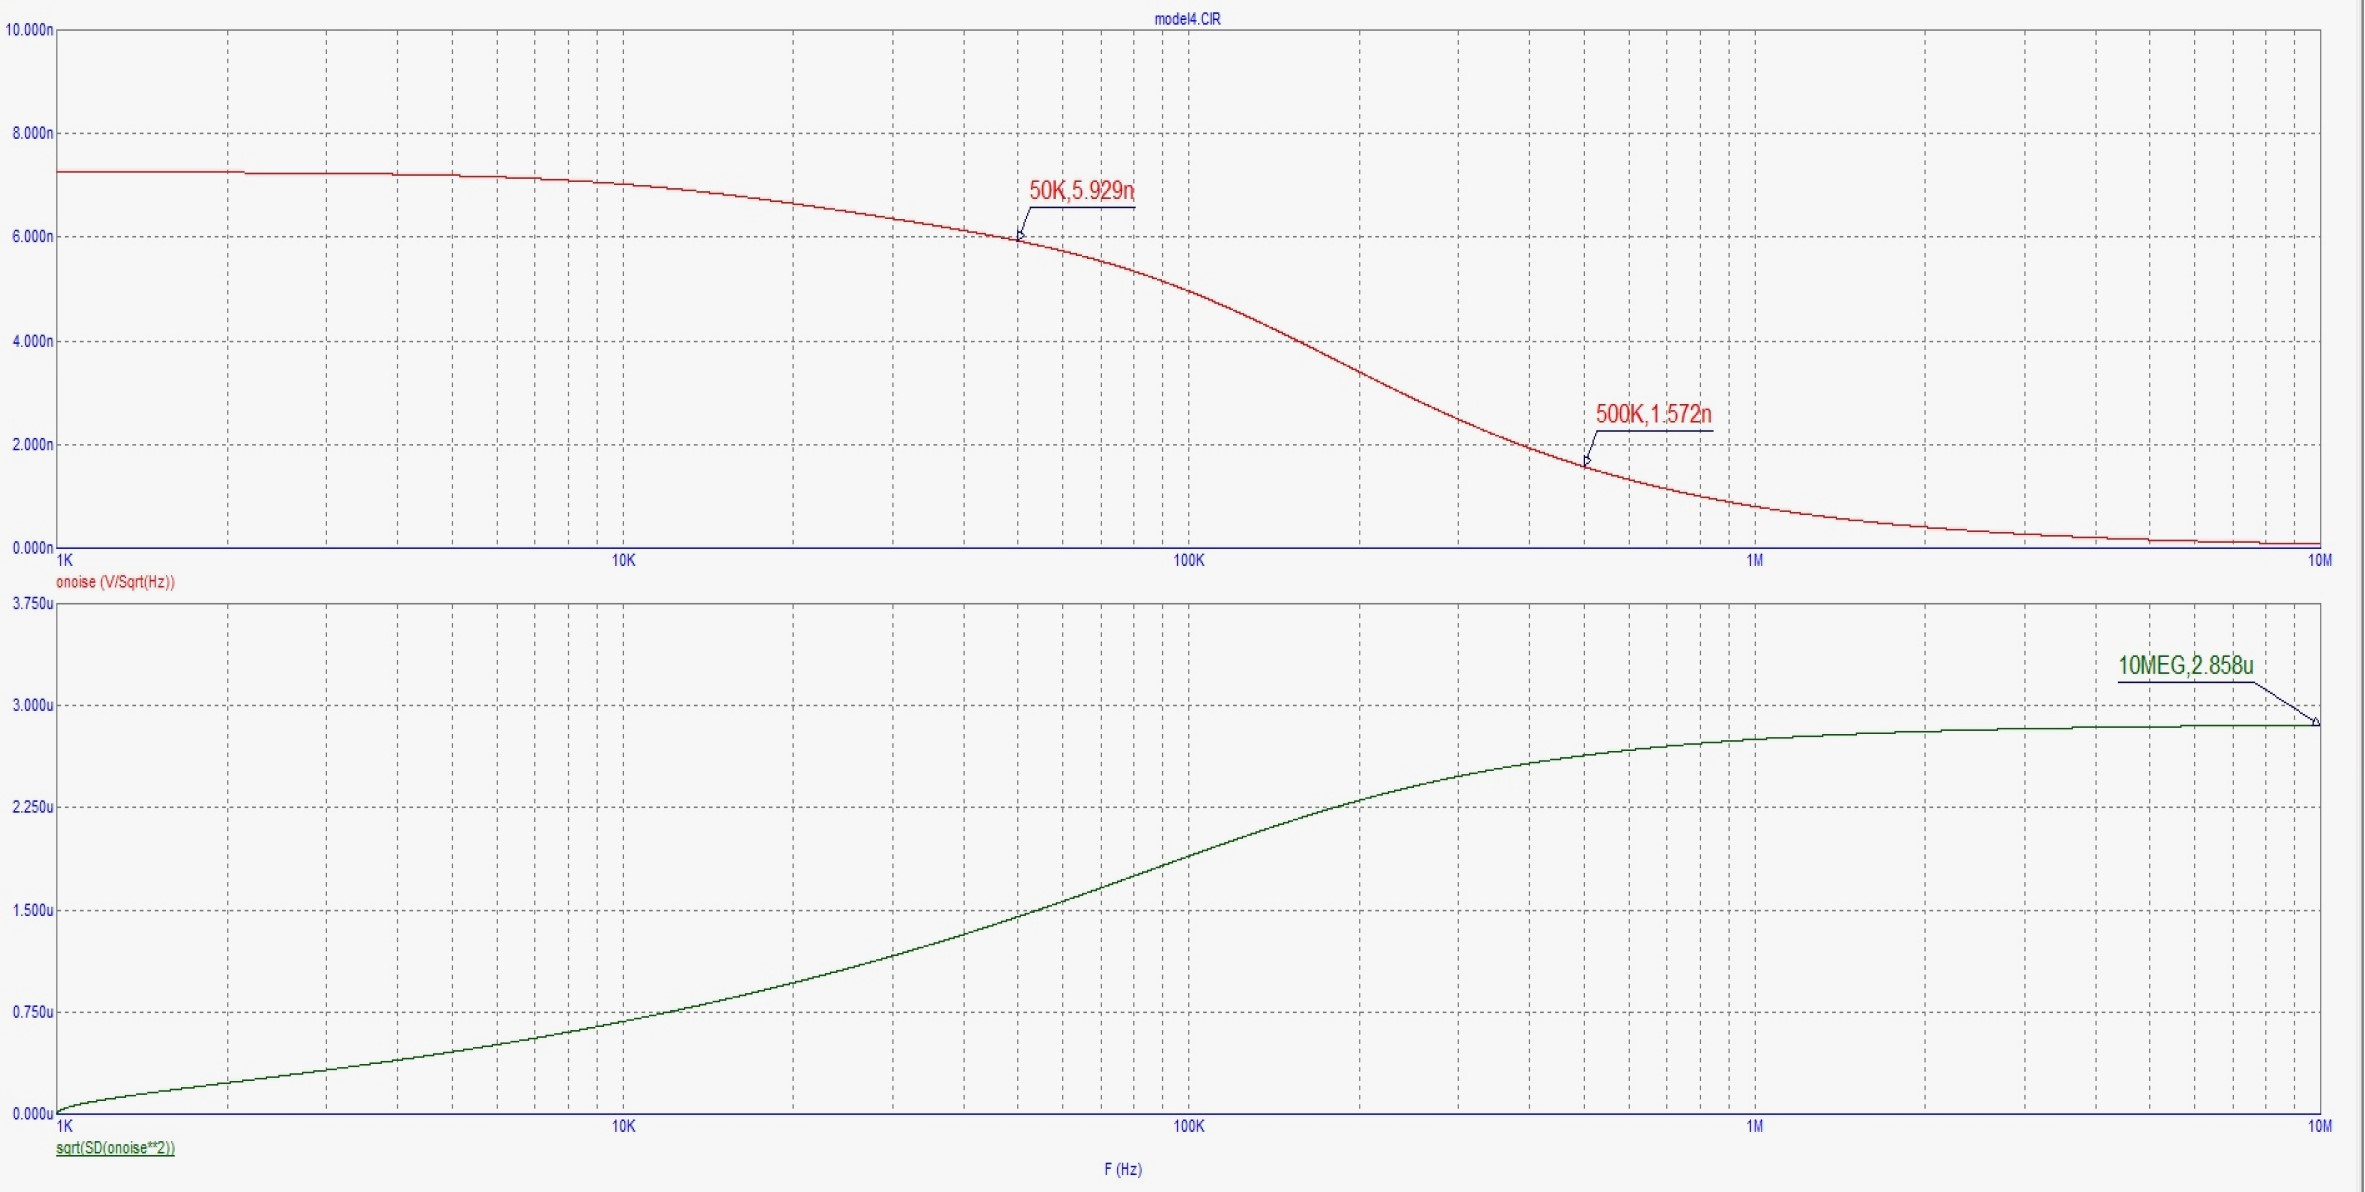
\includegraphics[width=1.1\linewidth]{4/4_2_3.jpg}
			\caption{Задание 4.2, пункт 2}
			\label{A}
\end{figure}



\begin{figure}[h!]
			\centering
			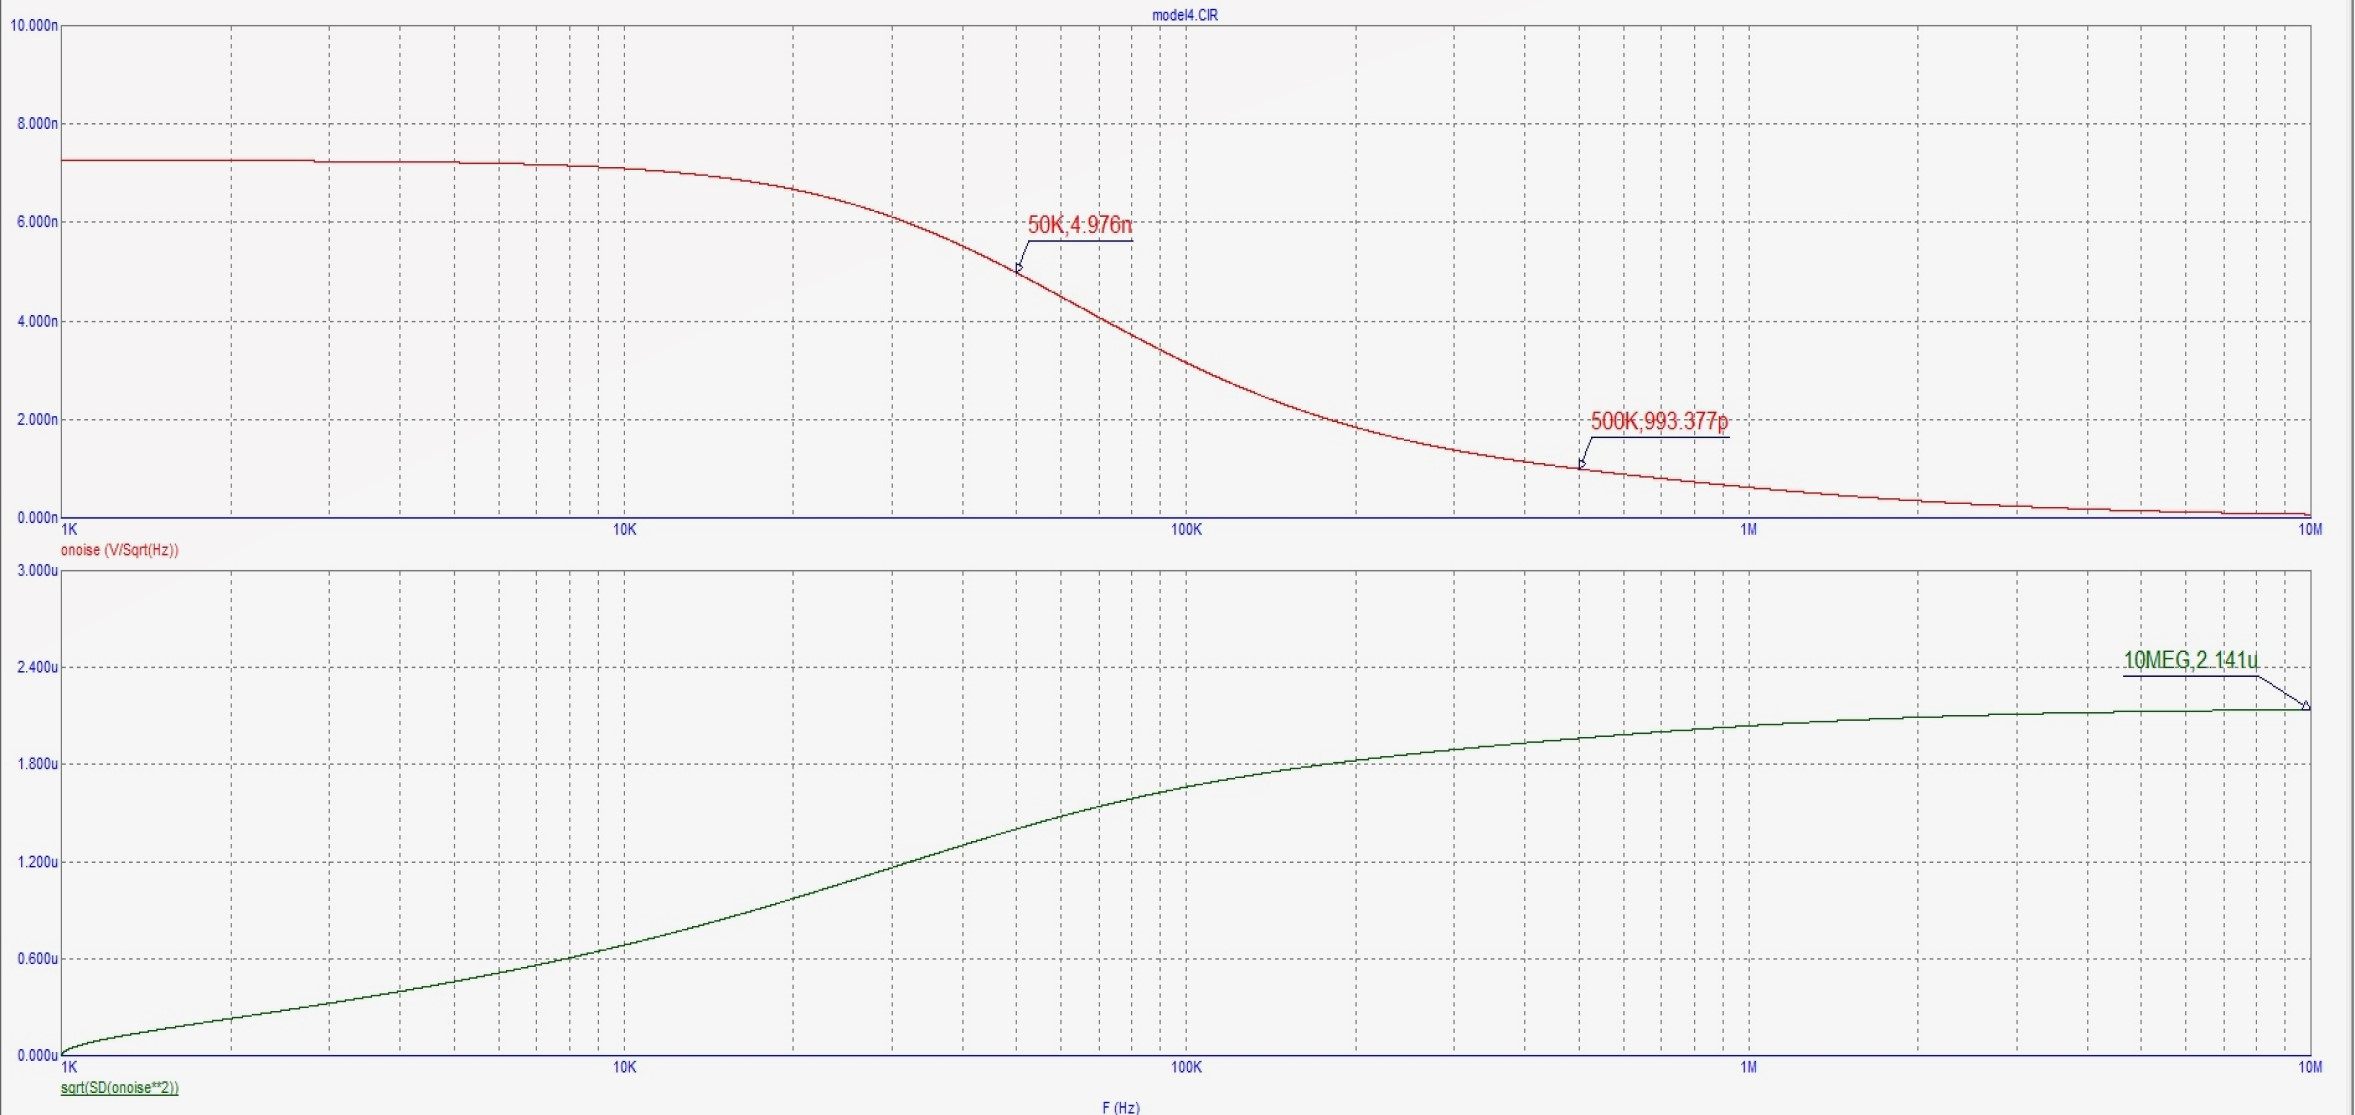
\includegraphics[width=1.1\linewidth]{4/4_2_5.jpg}
			\caption{Задание 4.2, пункт 2}
			\label{A}
\end{figure}




\begin{figure}[h!]
			\centering
			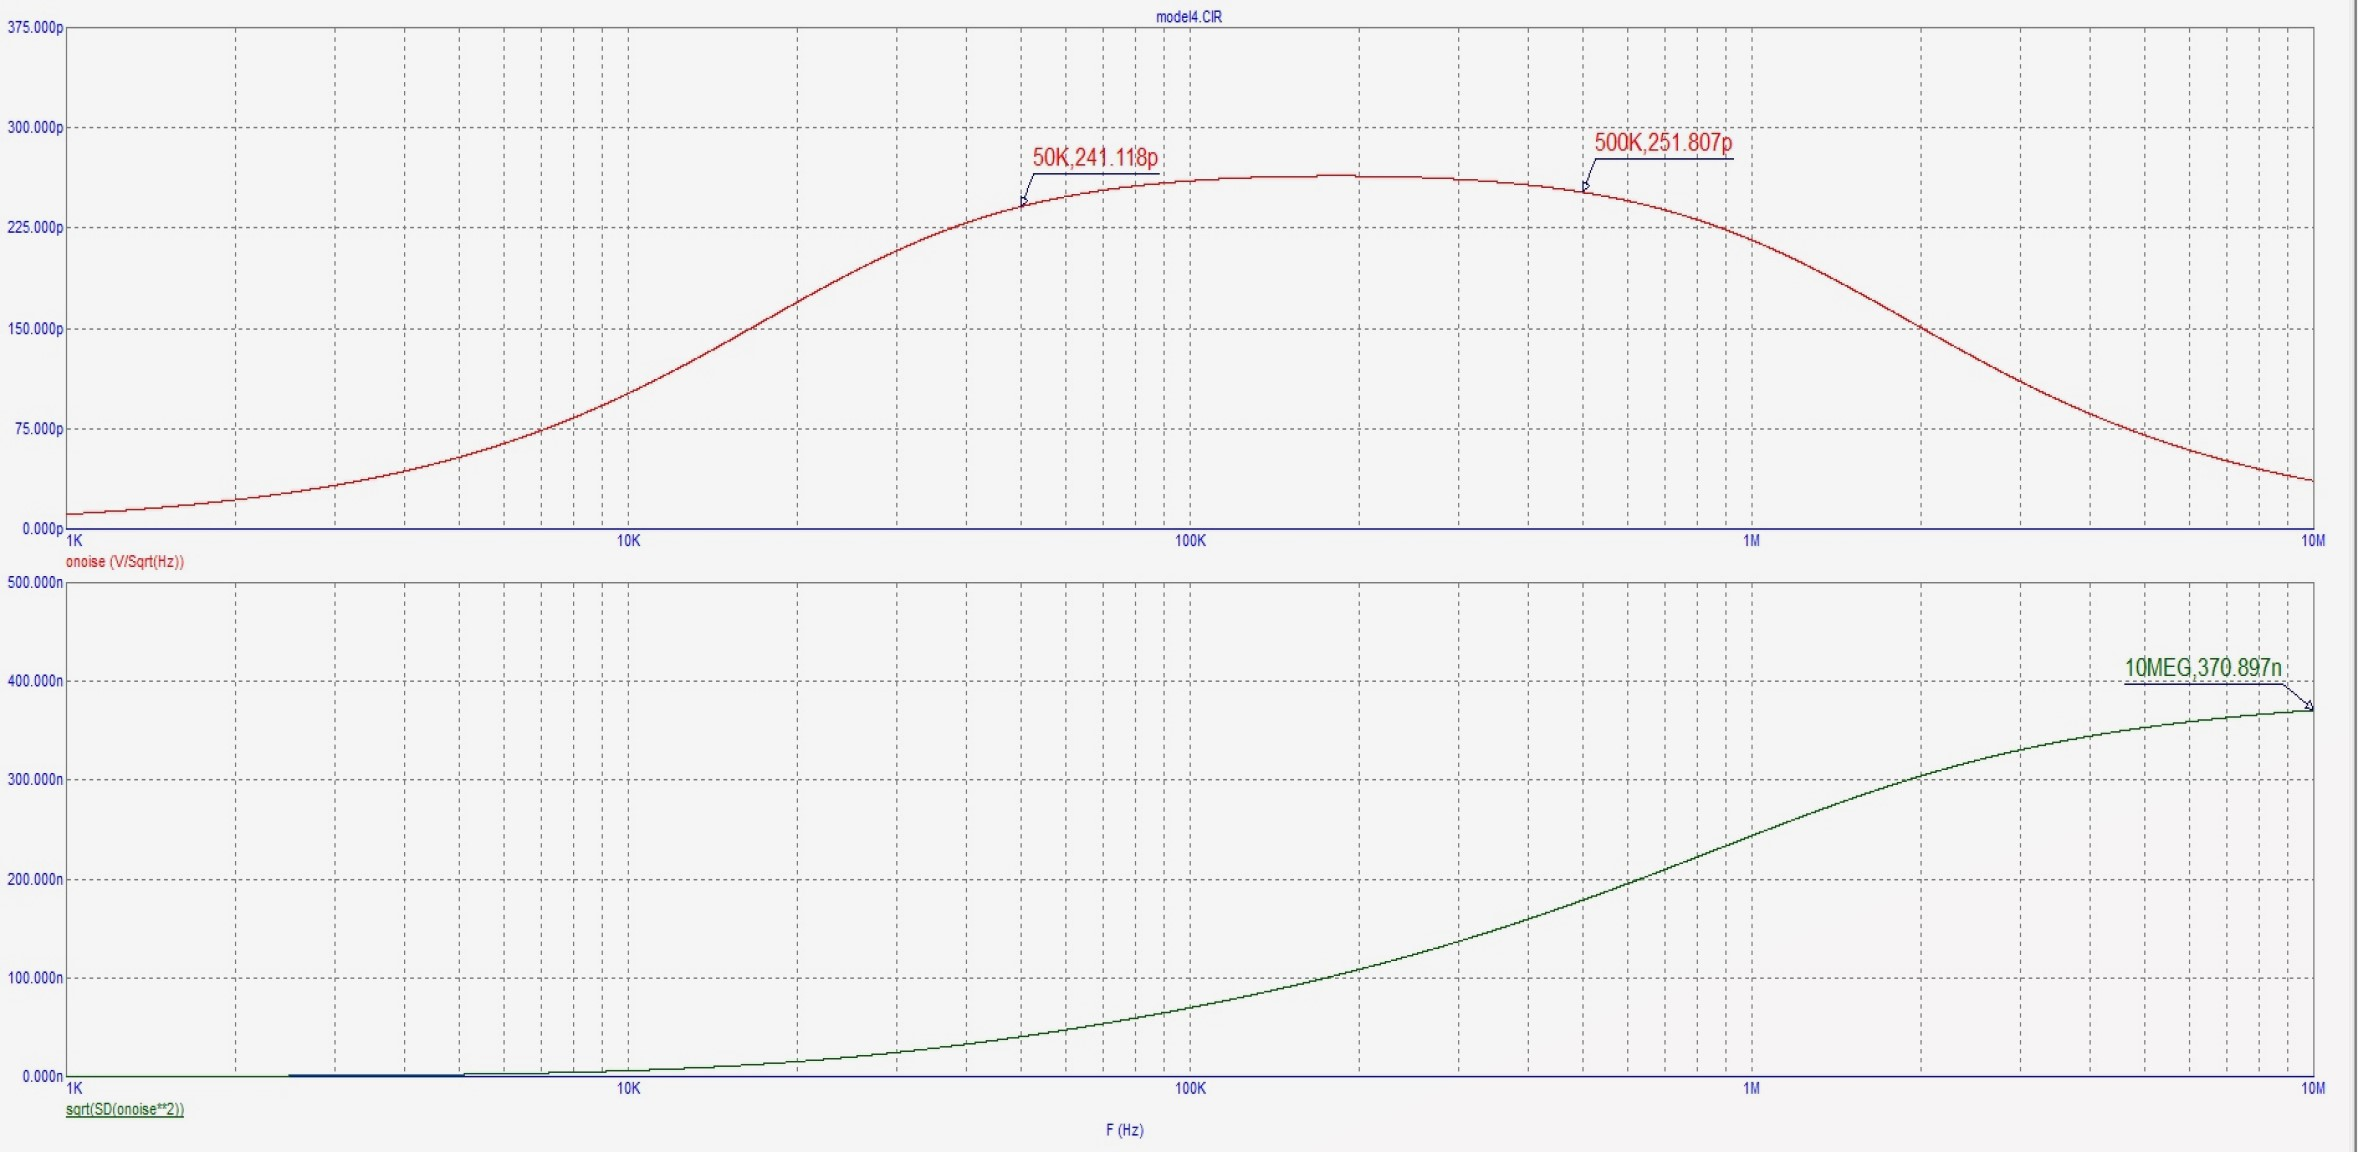
\includegraphics[width=1.1\linewidth]{4/4_2_4.jpg}
			\caption{Задание 4.2, пункт 2}
			\label{A}
\end{figure}

$\textbf{3.} $


По графику рис.41 оцениваем значение коэффициента шума на частотах $f_0$, $10f_0$, $f_0/100$ по формуле


\[  K_n = 20lg\frac{e_n(f)}{\sqrt{4kTR}}   \]


1) $e_{f_0}= 17.787n \Rightarrow K_n(f_0) = 7.8 $

2) $e_{f_0/100}= 726n \Rightarrow K_n(f_0/100) = 40 $

3) $e_{f_0/10}= 74.46n \Rightarrow K_n(f_0/10) = 20.2 $


\begin{figure}[h!]
			\centering
			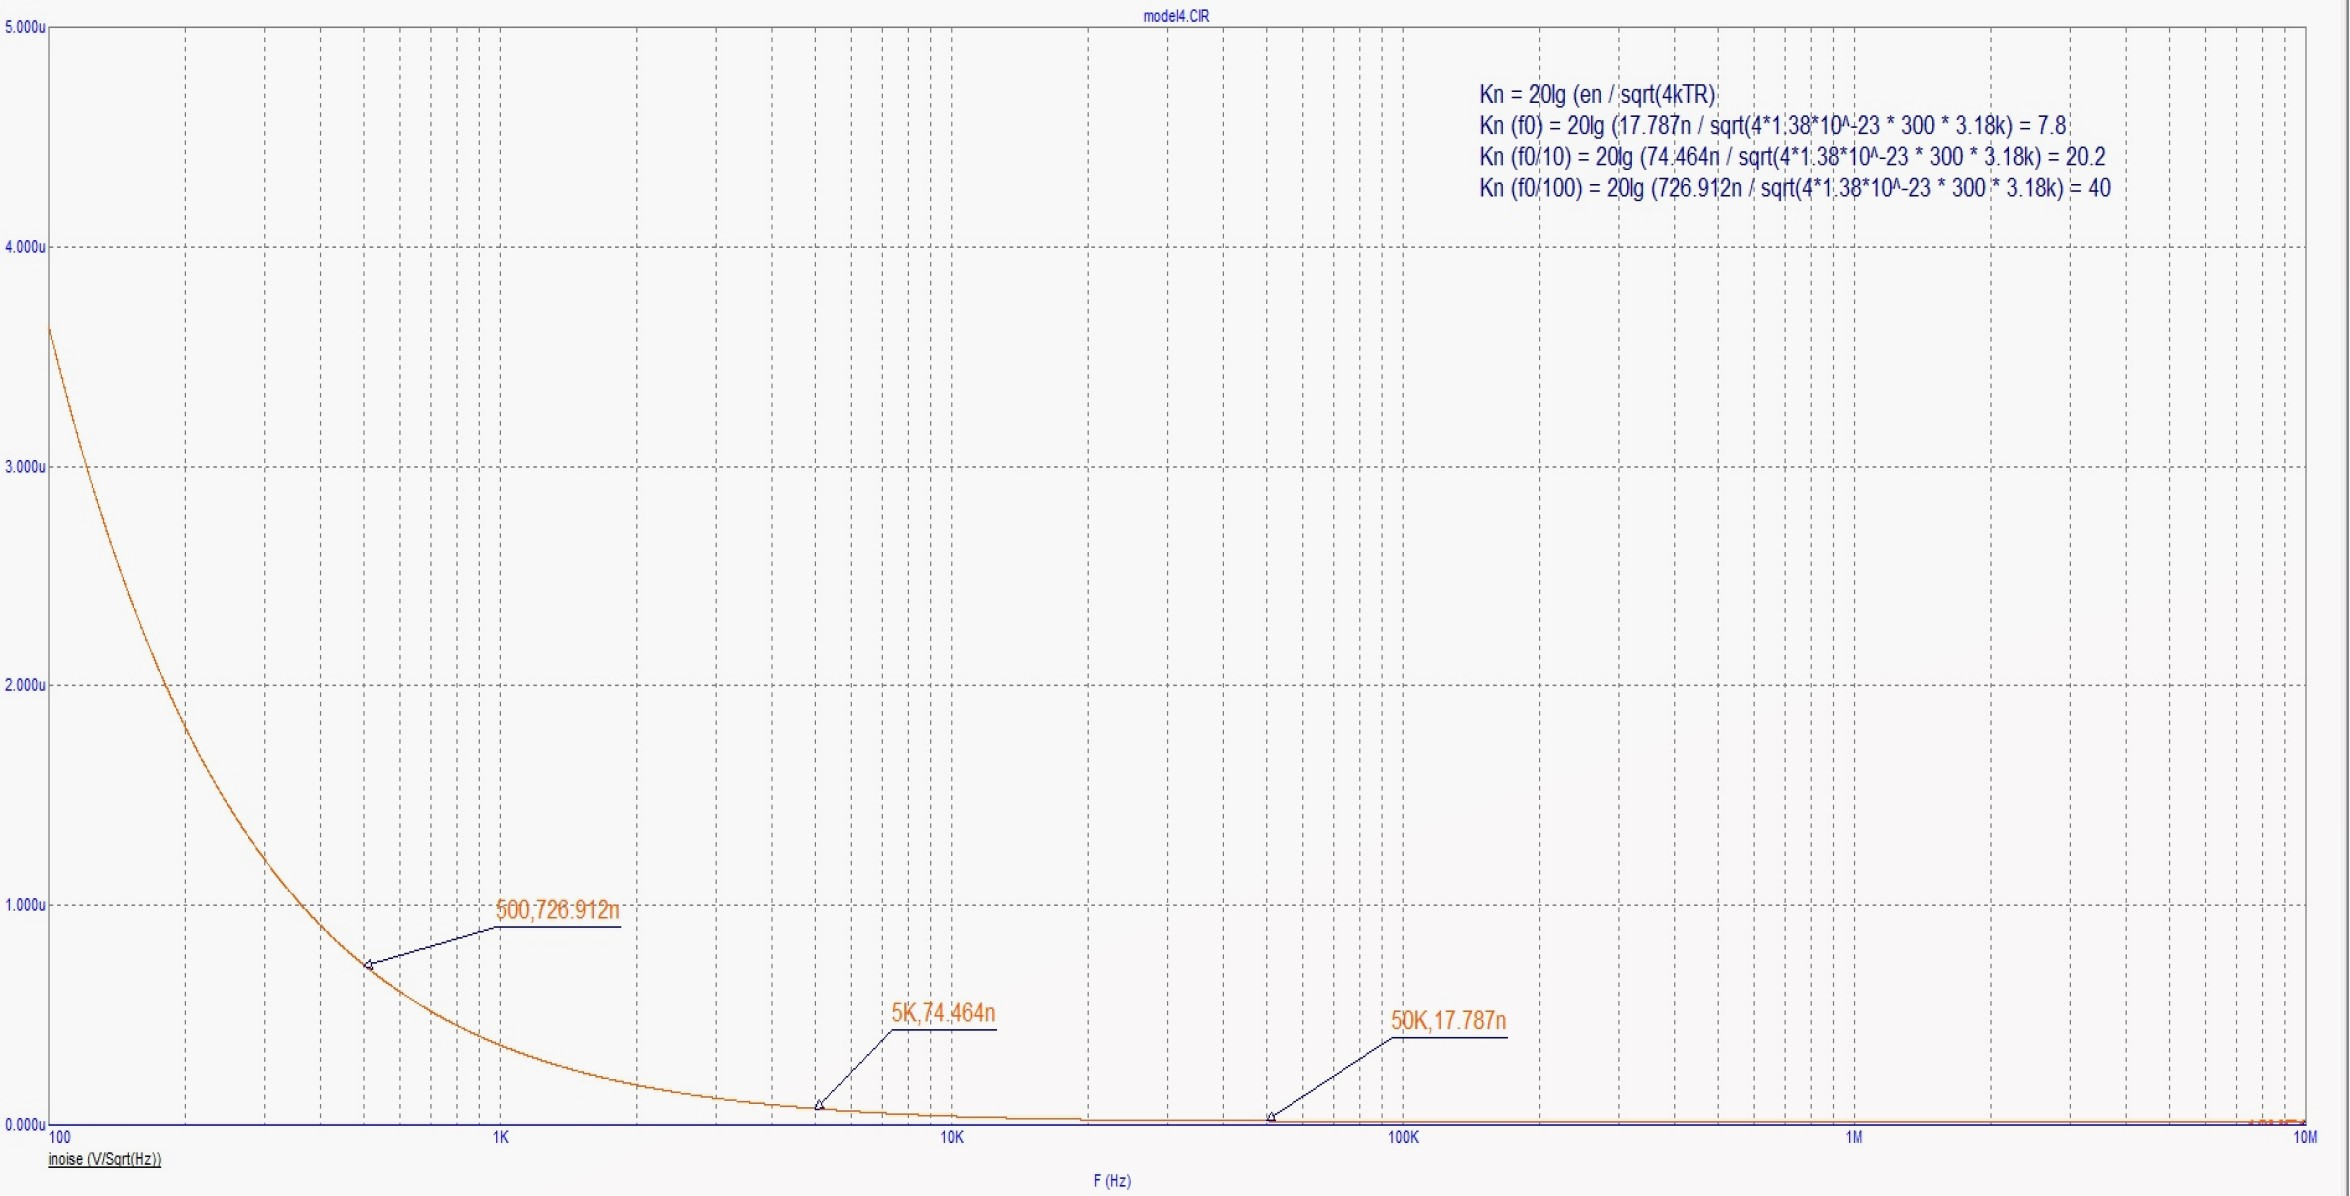
\includegraphics[width=1.1\linewidth]{4/4_2_1.jpg}
			\caption{Задание 4.2, пункт 3}
			\label{A}
\end{figure}



\subsection{$LC$--фильтр нижних частот}

$ $

$\textbf{1.} $

Подключив $v(n_3)/(v(V3)$ снимем АЧХ фильтра. Измерим резонансную частоту $f_0$, полосу по уровню 0.7, коэффициент передачи на резонансной и нулоевой частотах.

Сравним с теорией.

1) $f_0 = 102k, \: \Delta f = 34k$.

2) По графику:$K_{f_0} \approx 0.5$.
3) Теоретический расчет по формуле:

\[ K = \frac{0.5}{1 + jQ\cdot(\frac{f}{f_0} - \frac{f_0}{f})}\]

Получаем, что $K_1 = 0.5$.

С теорией совпало.

\begin{figure}[h!]
			\centering
			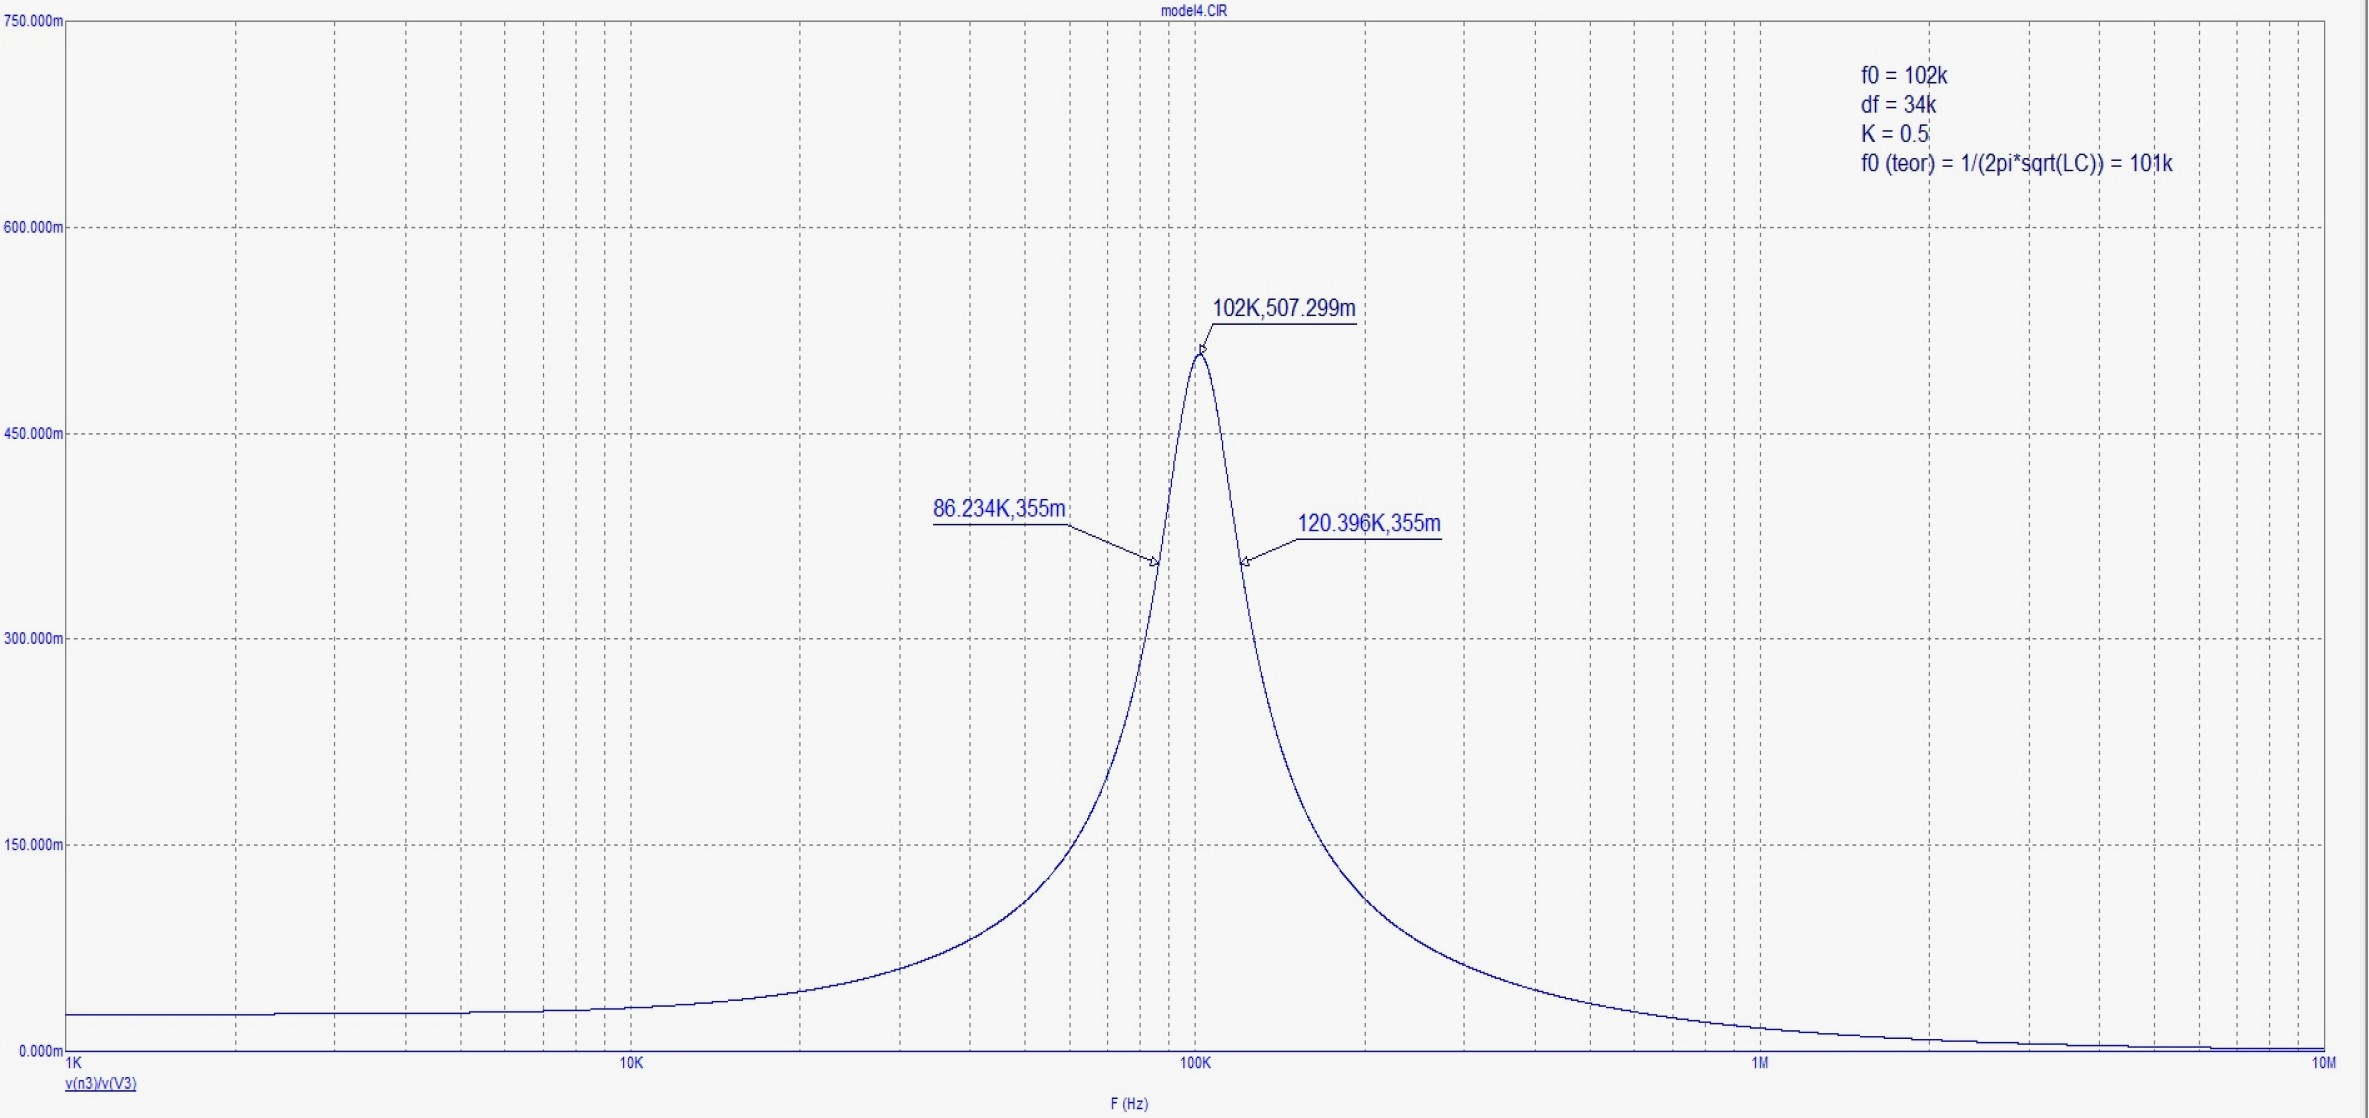
\includegraphics[width=1.1\linewidth]{4/4_3_2.jpg}
			\caption{Задание 4.3, пункт 1}
			\label{A}
\end{figure}


$\textbf{2.} $


Измерим уровни шумвого напряжения на частотах $f_0, f_0/100$. Так же заменим поочередно первый и второй резисторы нешумящим сопротивлением $H_1$, оценим вклад шумов $R_{s3}, R_3$ в шумовое напряжение и в уровень шума на выходе:
1) $n_{f_0} = 7.963n, \: n_{\frac{f_0}{10}} = 1.841n, \: \sigma = 1.819u$

2) $n_{f_0} = 5.335n, \: n_{\frac{f_0}{10}} = 344p, \: \sigma = 1.265u$

3) $n_{f_0} = 344.8p, \: n_{\frac{f_0}{10}} = 944p, \: \sigma = 230n$

\begin{figure}[h!]
			\centering
			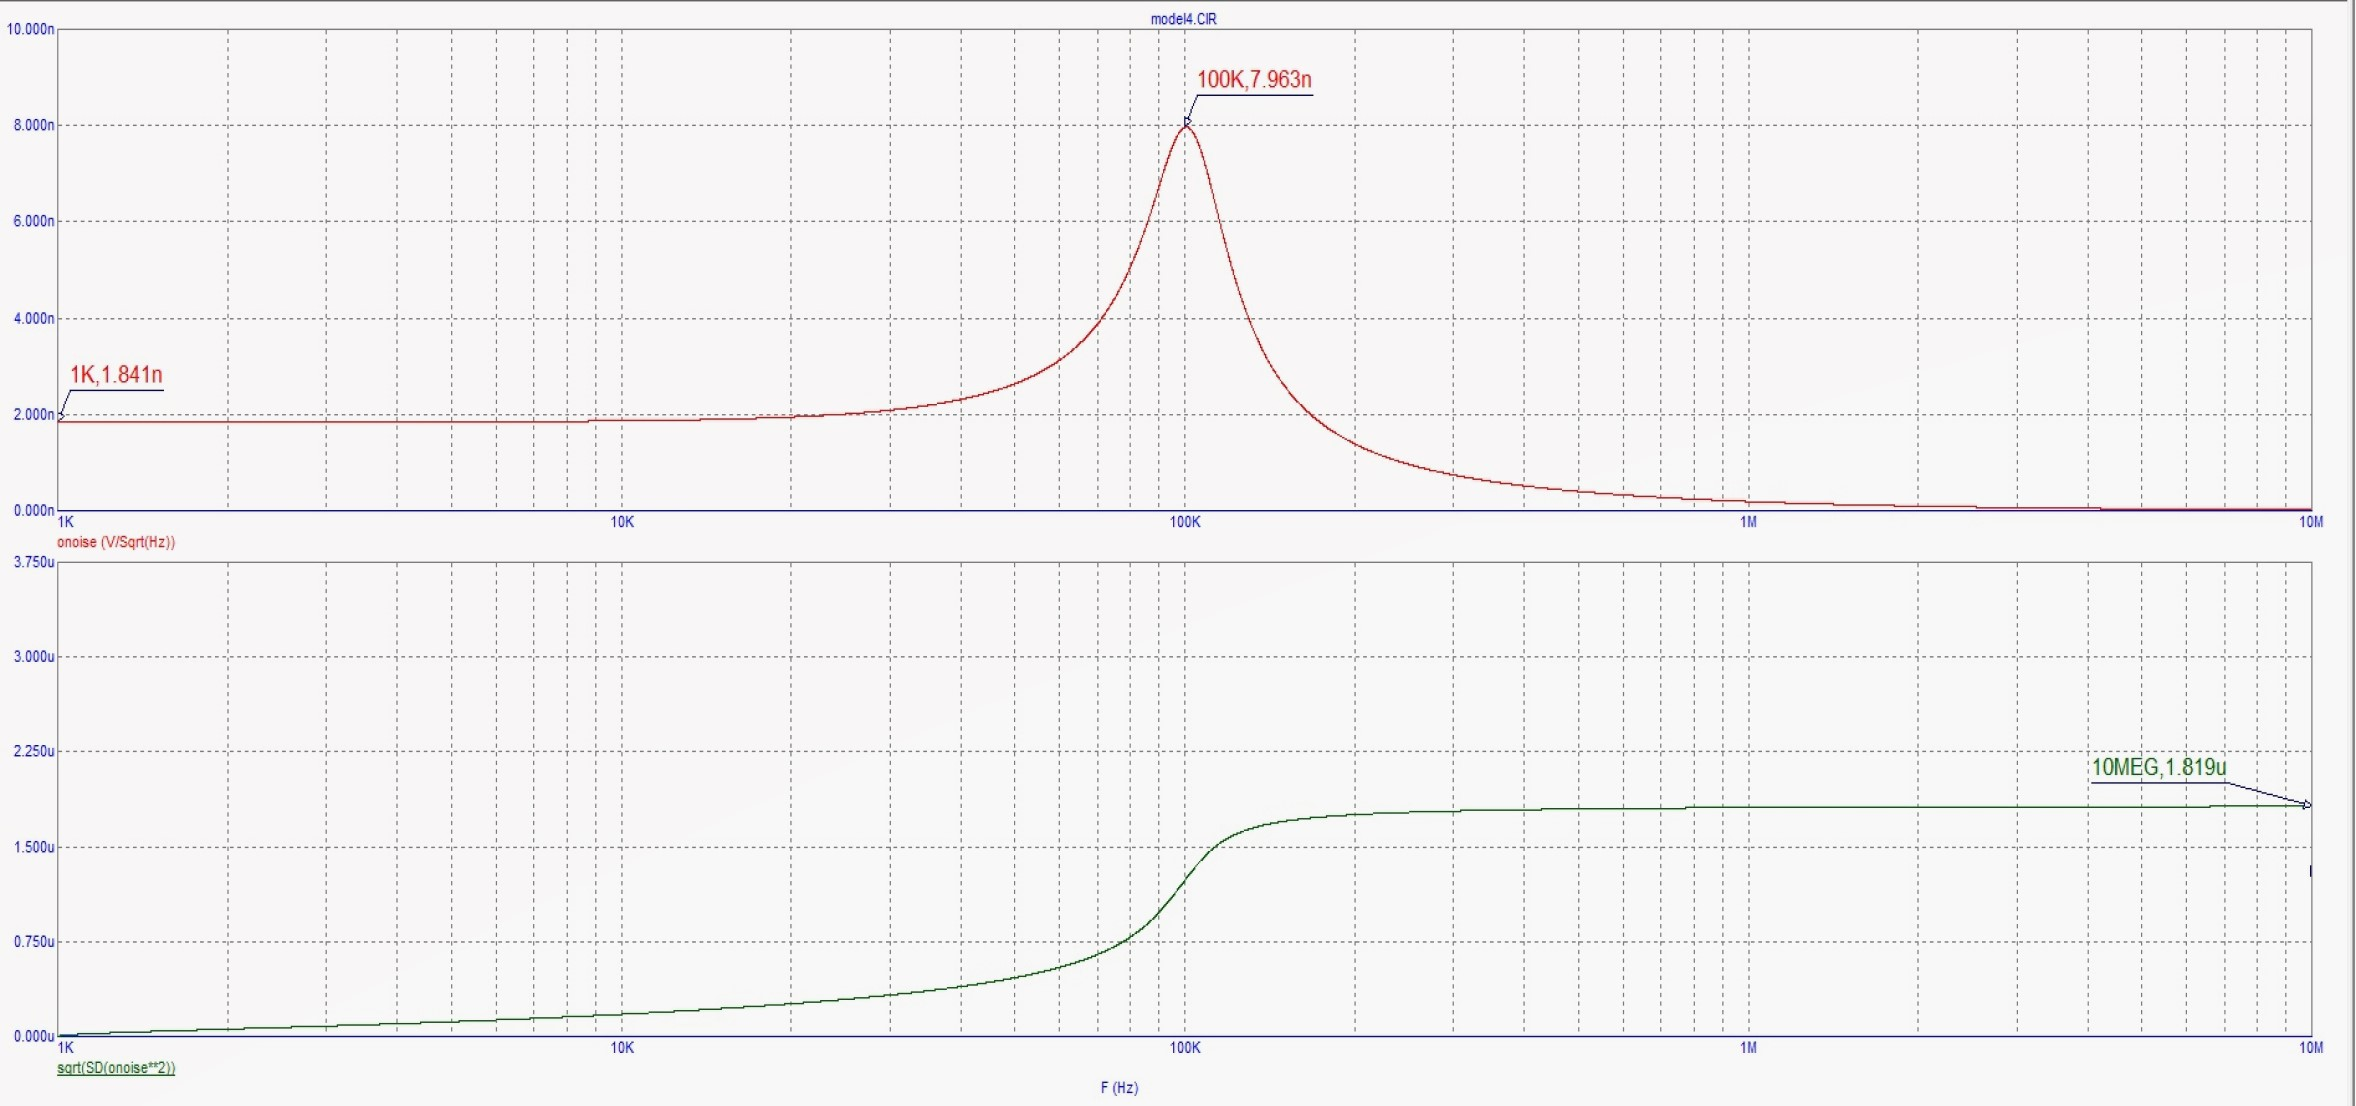
\includegraphics[width=1.1\linewidth]{4/4_3_3.jpg}
			\caption{Задание 4.3, пункт 2}
			\label{A}
\end{figure}



\begin{figure}[h!]
			\centering
			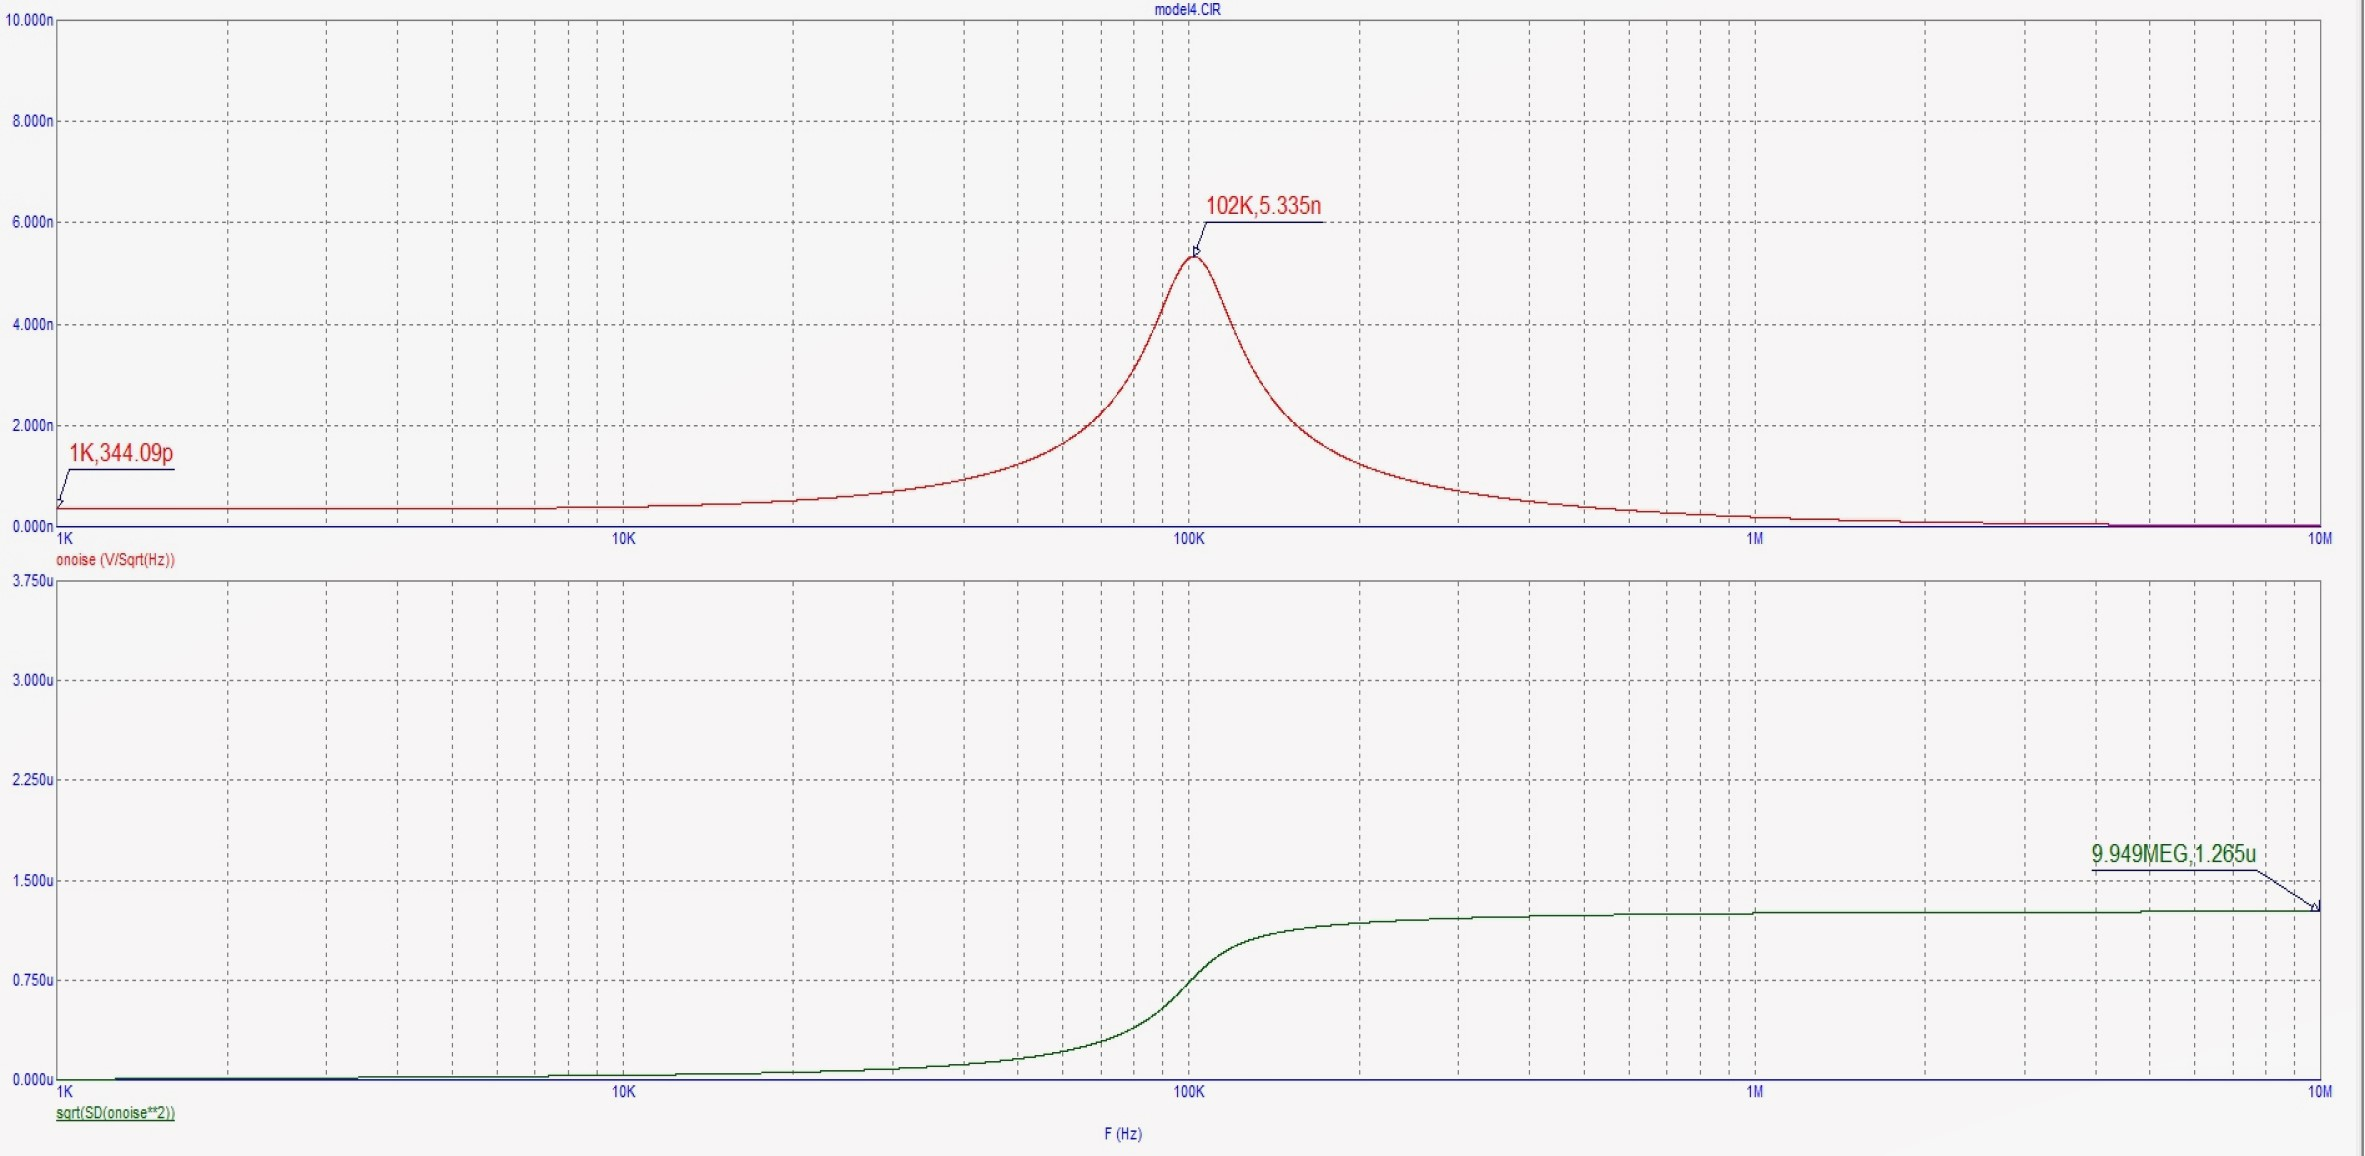
\includegraphics[width=1.1\linewidth]{4/4_3_4.jpg}
			\caption{Задание 4.3, пункт 2}
			\label{A}
\end{figure}

\begin{figure}[h!]
			\centering
			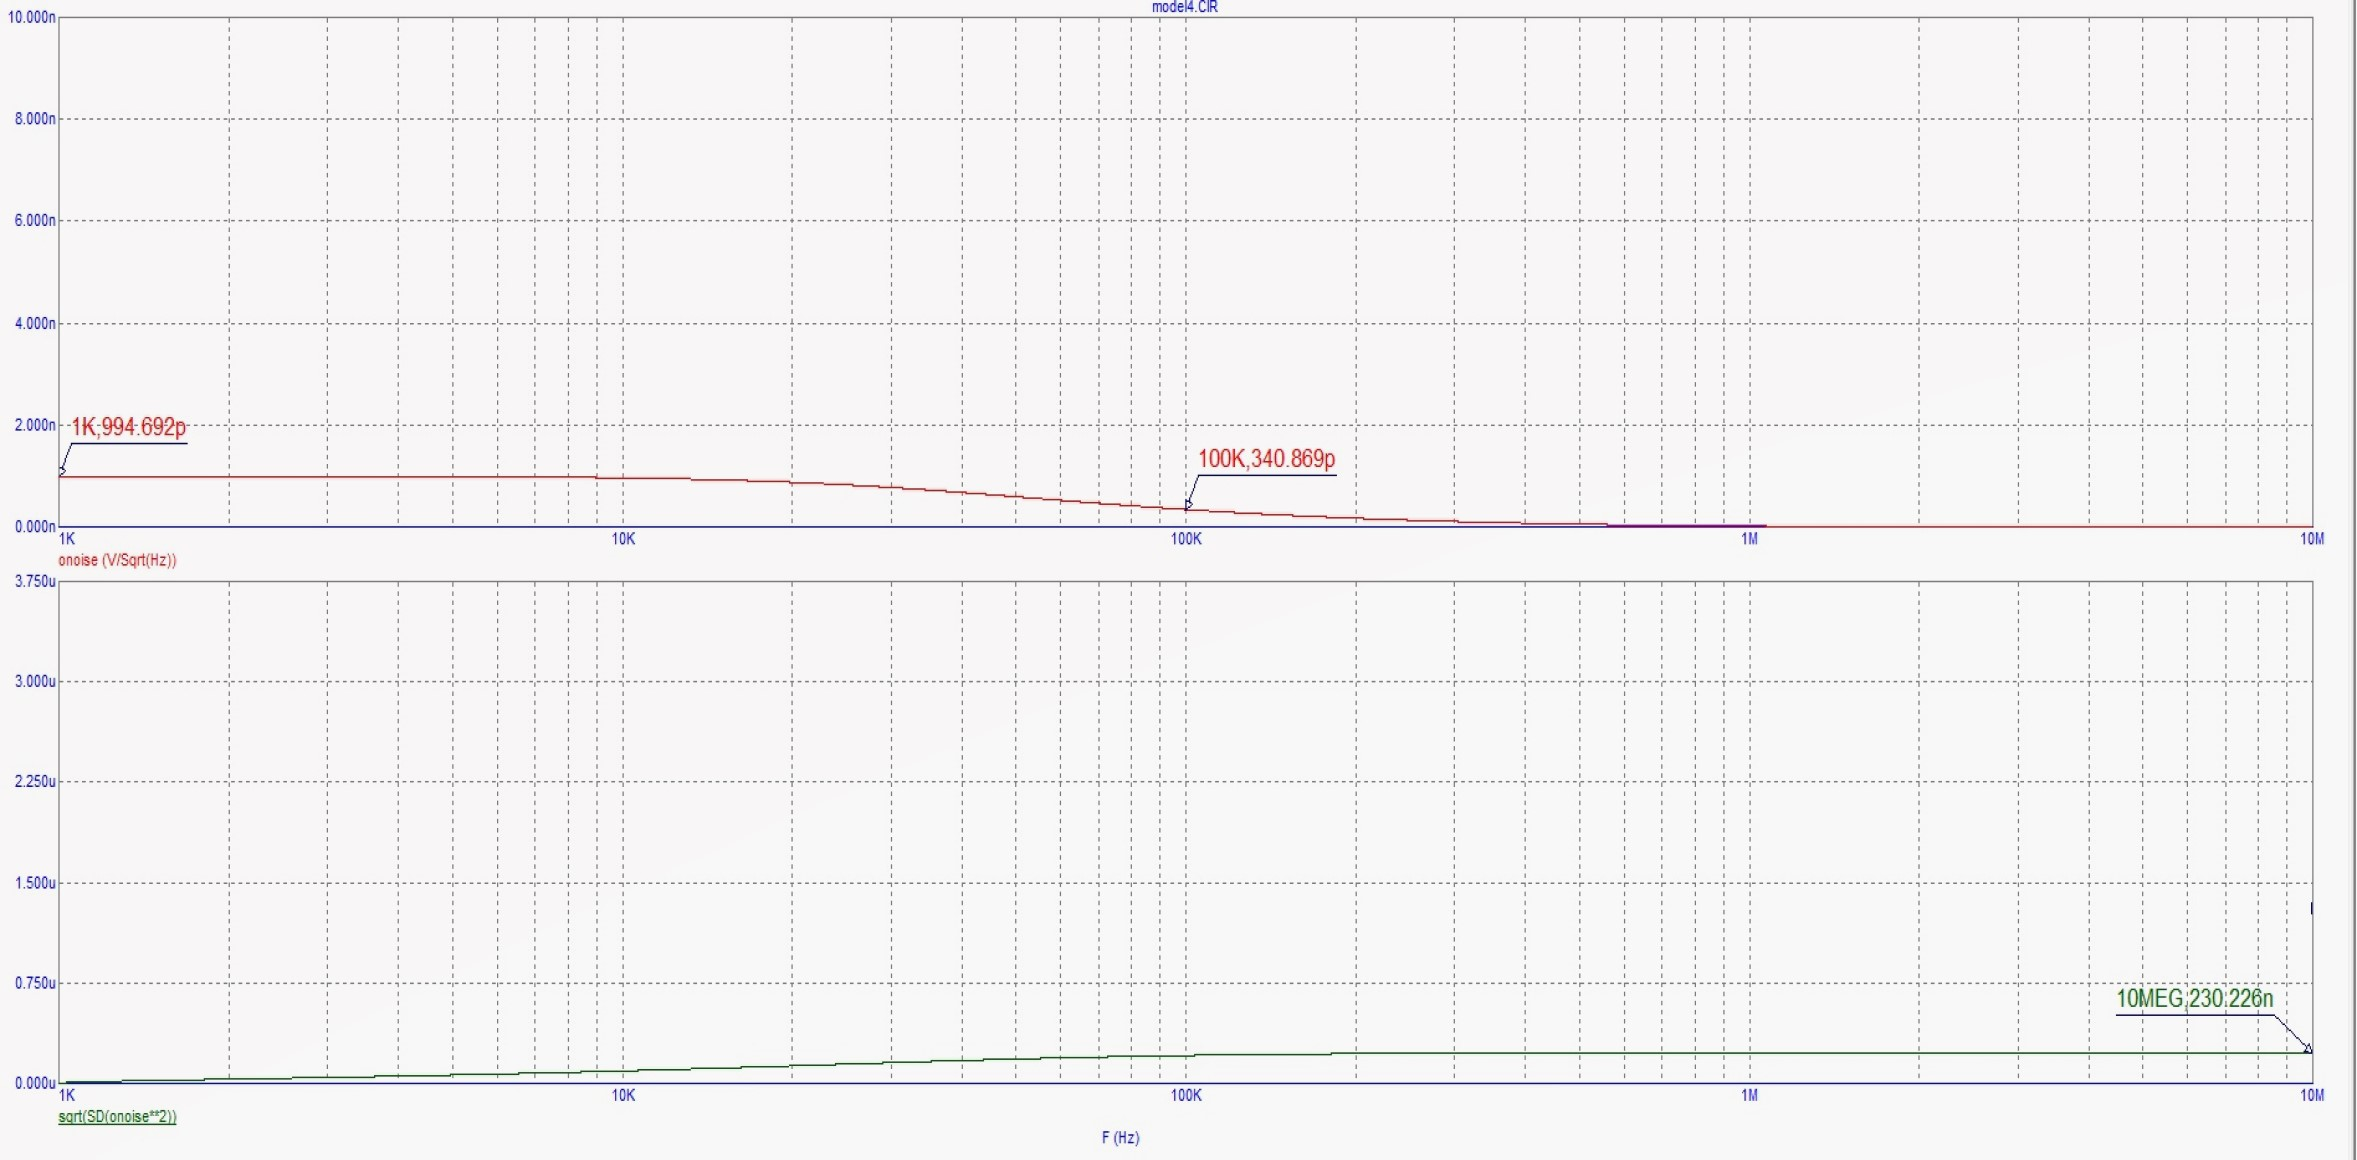
\includegraphics[width=1.1\linewidth]{4/4_3_5.jpg}
			\caption{Задание 4.3, пункт 2}
			\label{A}
\end{figure}


$\textbf{3.} $

По графику рис.46 оцениваем значение коэффициента шума на частотах $f_0$, $10f_0$, $f_0/100$ по формуле


\[  K_n = 20lg(\frac{e_n(f)}{\sqrt{4kTR}})   \]


1) $e_{f_0}= 68.329n \Rightarrow  K_n(f_0) = 18.6 $

2) $e_{f_0/100}= 15.806n \Rightarrow K_n(f_0/100) = 31.3$

3) $e_{10f_0}= 11.28n \Rightarrow  K_n(10f_0) = 15.6$


\begin{figure}[h!]
			\centering
			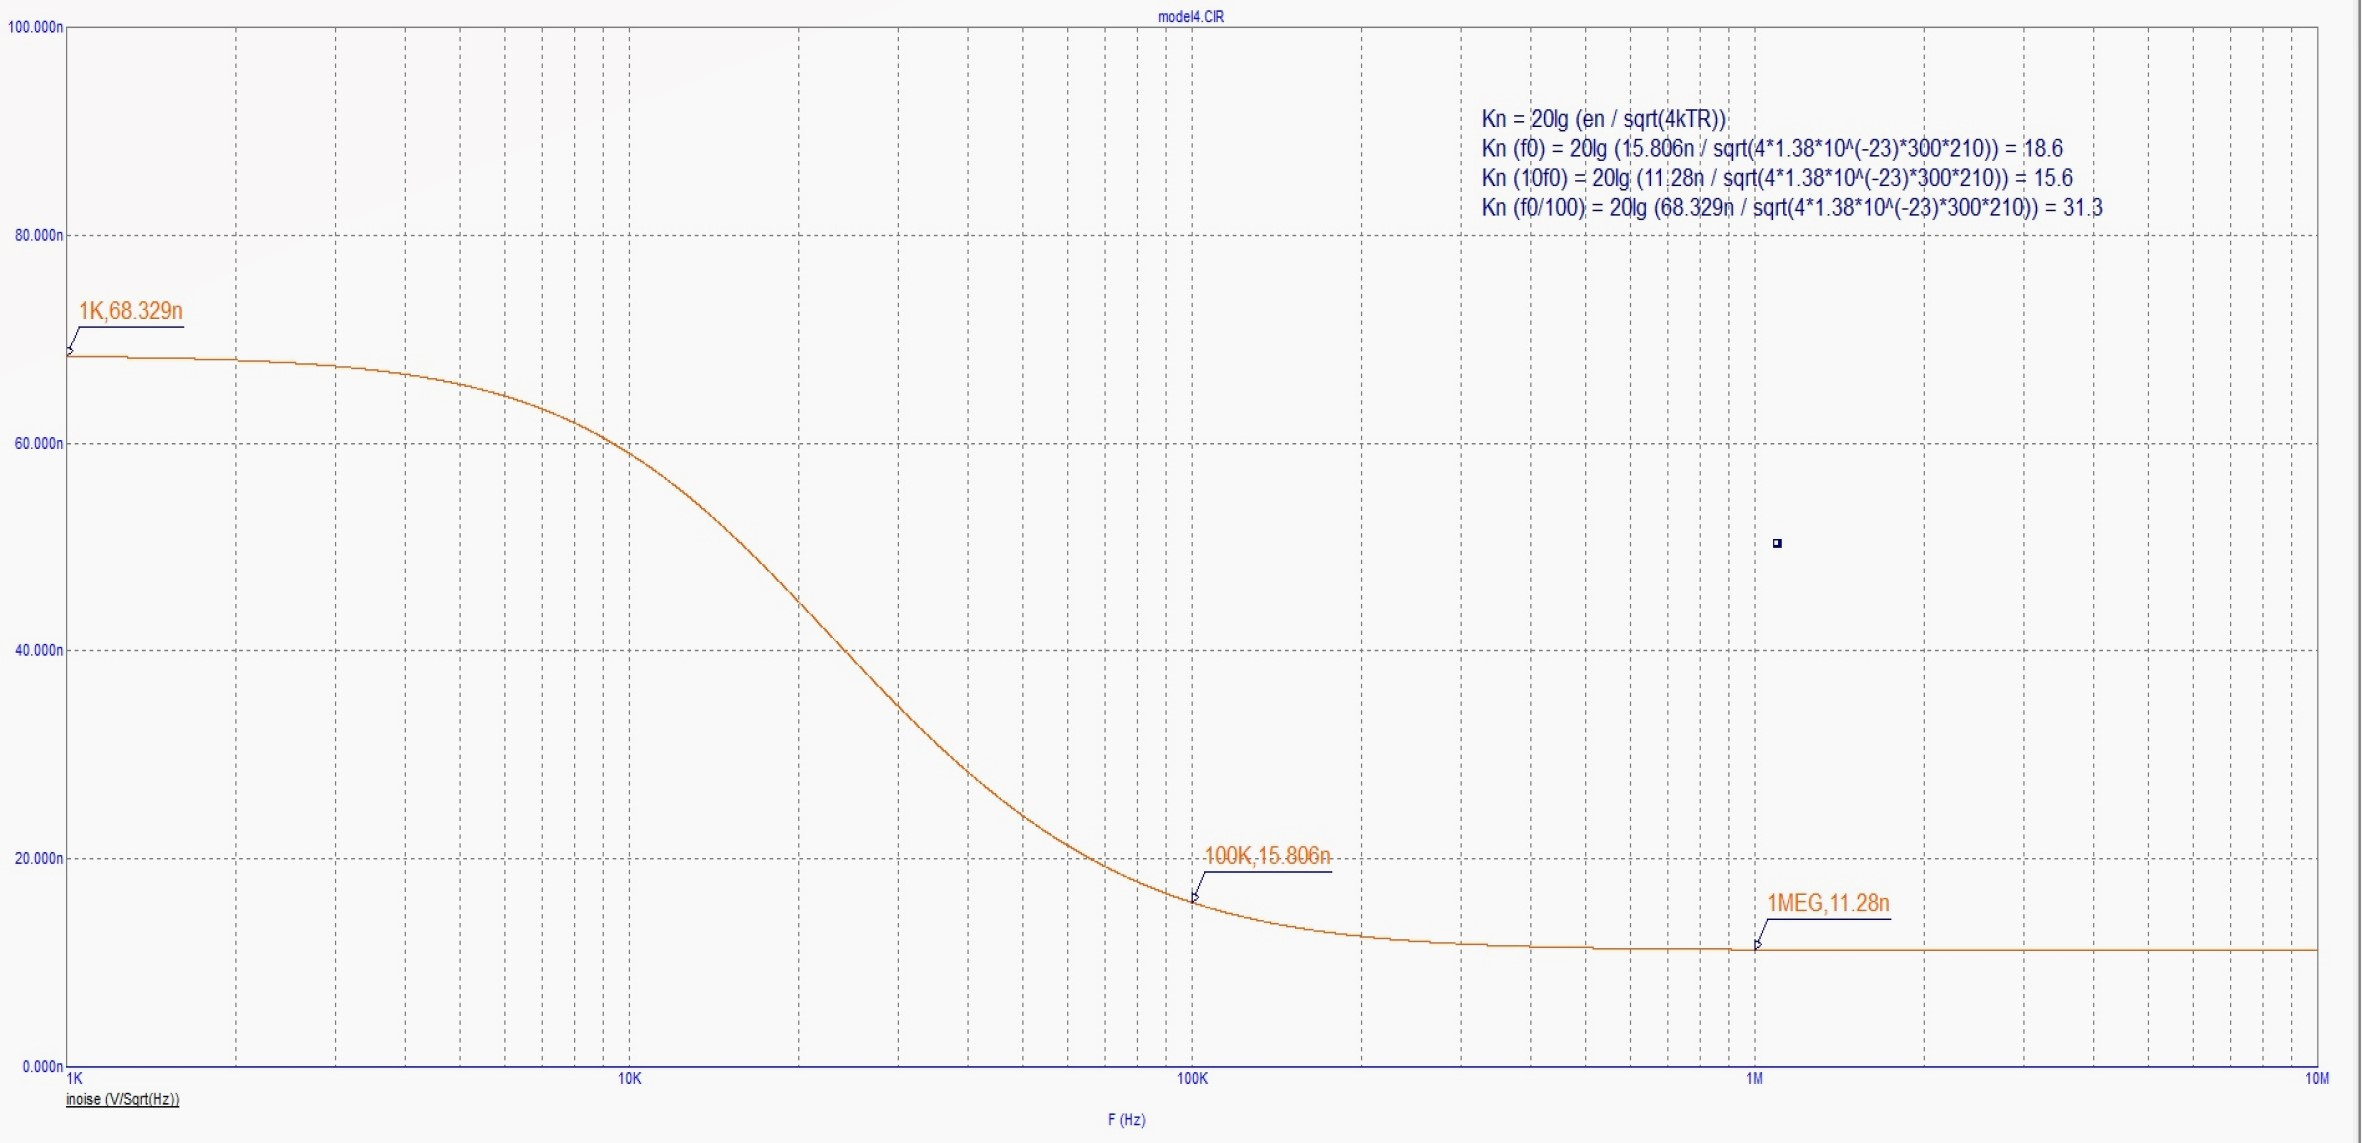
\includegraphics[width=1.1\linewidth]{4/4_3_1.jpg}
			\caption{Задание 4.3, пункт 3}
			\label{A}
\end{figure}


\newpage

\section{Шумы в усилителе на биполярном транзисторе}

$\textbf{1.}$


Установим ${E1/i}$

$I_c = 300u, \:B = 200Ohm, \: I1 = 13.5uA.$

\begin{figure}[h!]
			\centering
			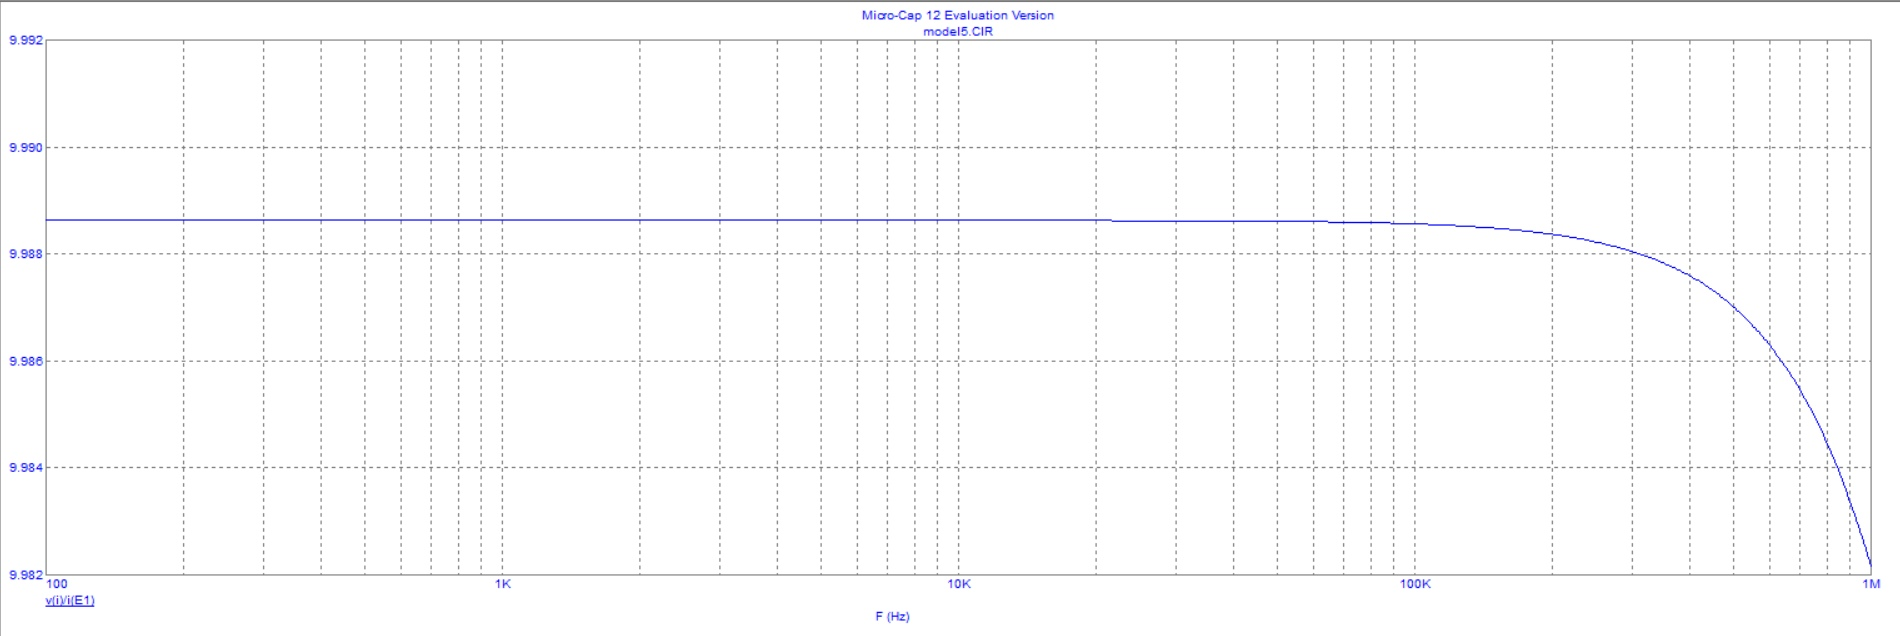
\includegraphics[width=1.1\linewidth]{5/5_1_1.jpg}
			\caption{Задание 5.1, пункт 1}
			\label{A}
\end{figure}

$\textbf{2.}$

Снимем зависимость $i(f)$ от $H_s$, варьируя $H_s[10, 1000k|log10]$, $RB = 0$

\begin{figure}[h!]
			\centering
			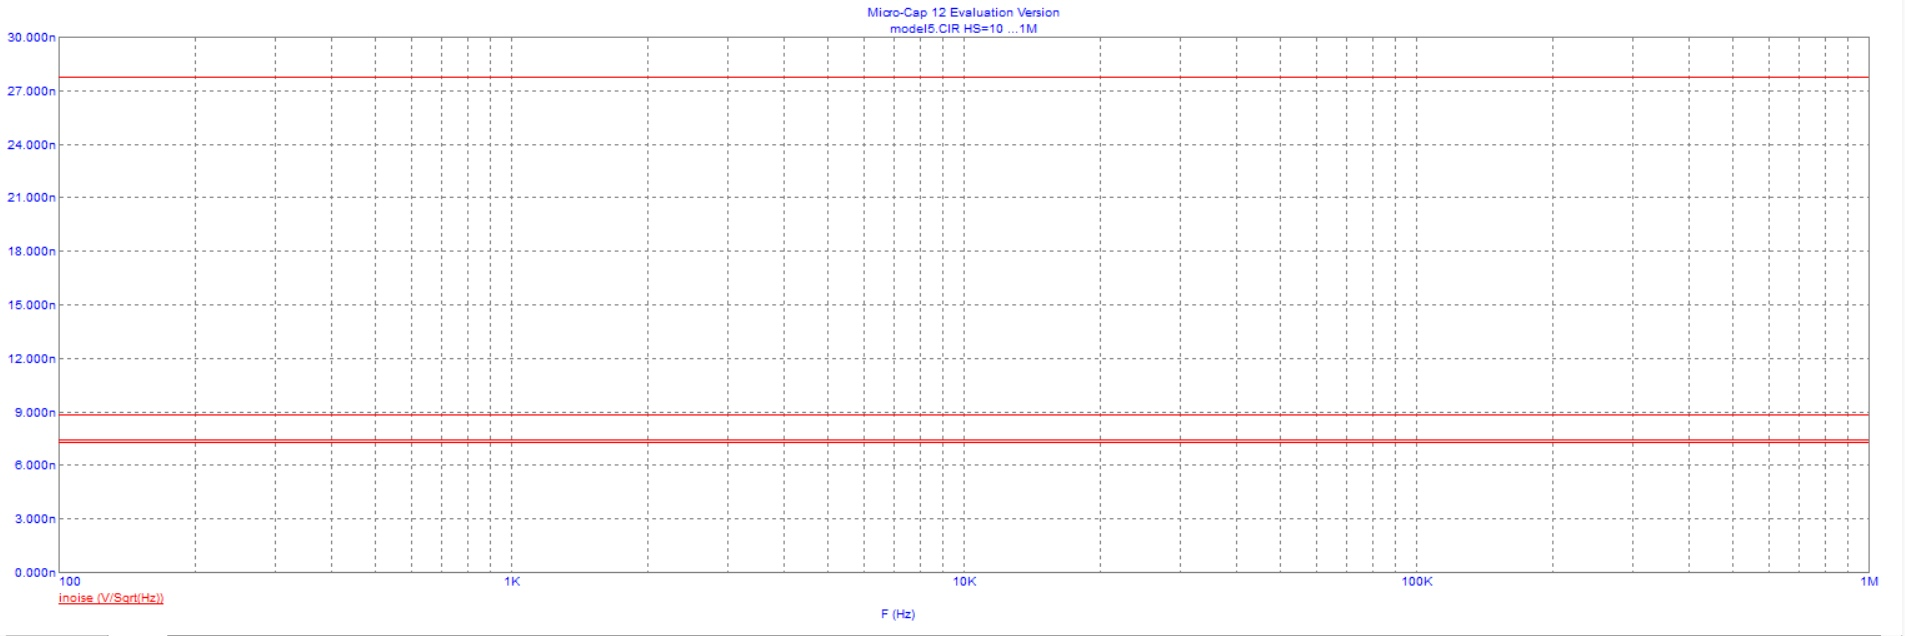
\includegraphics[width=1.1\linewidth]{5/5_1_2.jpg}
			\caption{Задание 5.1, пункт 2}
			\label{A}
\end{figure}

$H_s = 1M, i = 2.3u$

$H_s = 100k, i = 224.3n$

$H_s = 10k, i = 27.7n$

$H_s = 1k, i = 8.8n$

$H_s = 100, i = 7.4n$

$H_s = 10, i = 7.3n$

Снимем зависимость $i(f)$ от $H_s$, варьируя $RB[0, 100|25]$, $H_s = 0$

\begin{figure}[h!]
			\centering
			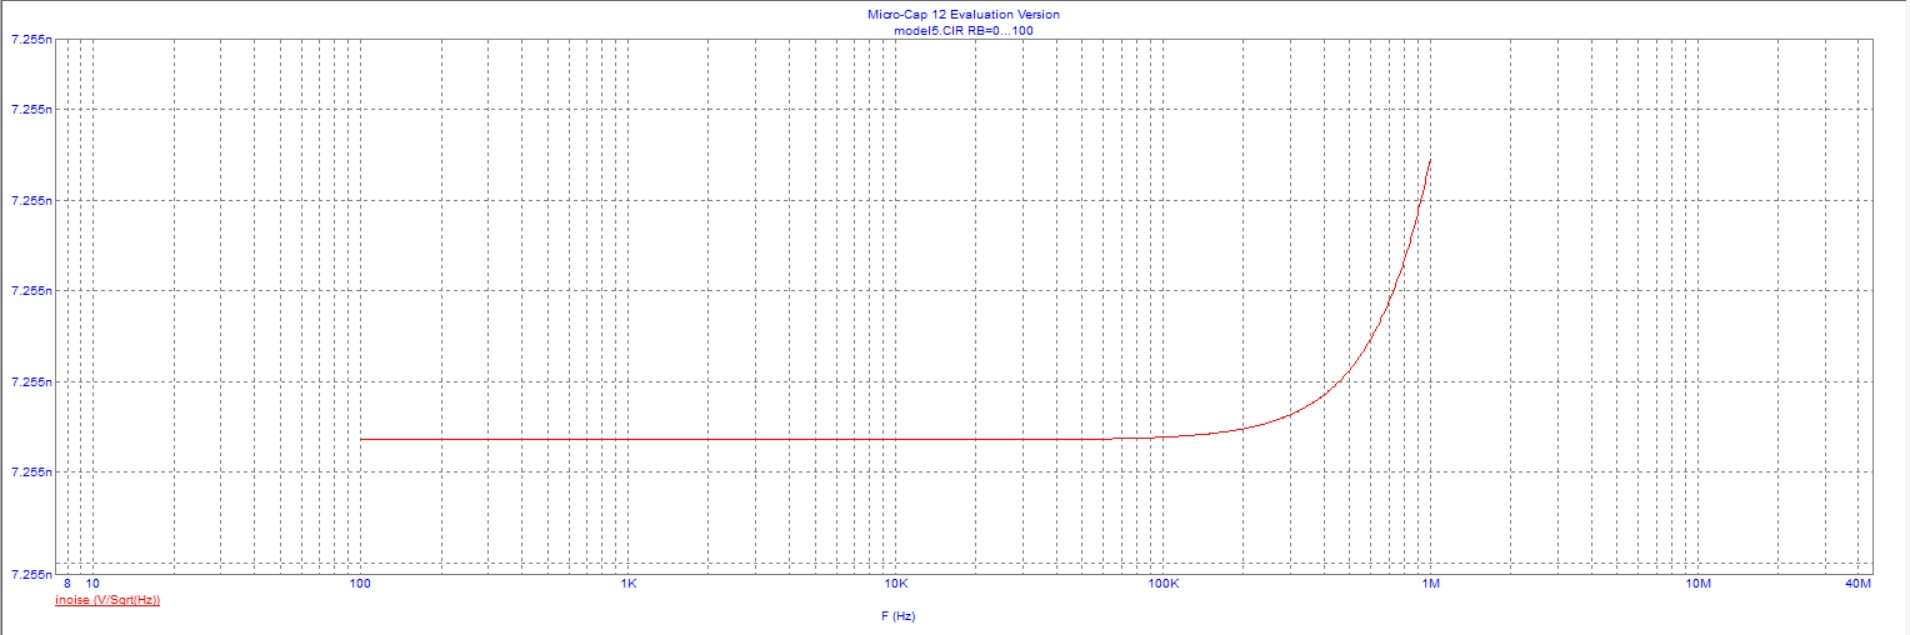
\includegraphics[width=1.1\linewidth]{5/5_1_3.jpg}
			\caption{Задание 5.1, пункт 2}
			\label{A}
\end{figure}

$\textbf{3.}$


Повторим измерения для $I_c = 0.1mA$

\begin{figure}[h!]
			\centering
			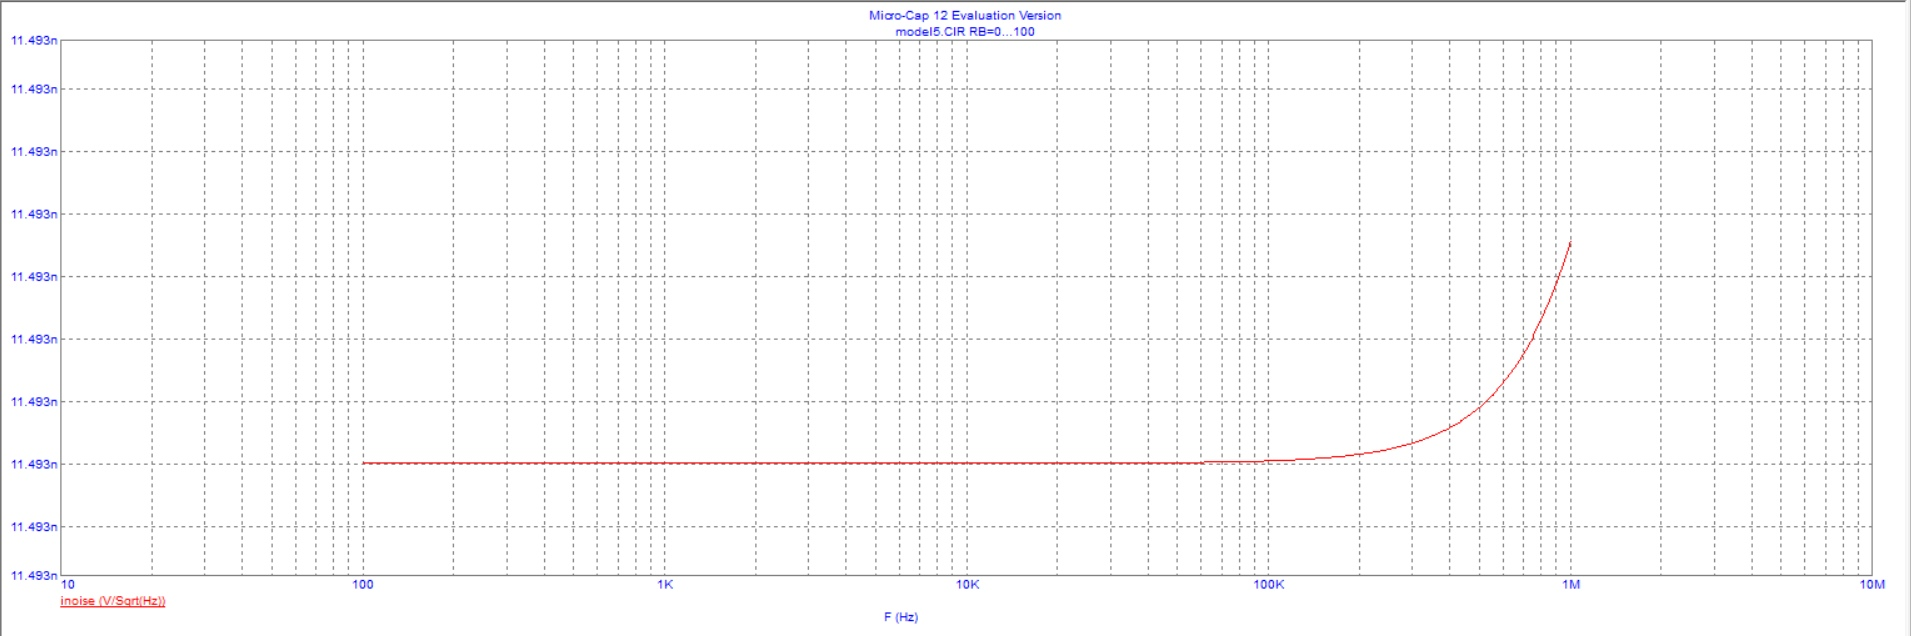
\includegraphics[width=1.1\linewidth]{5/5_1_4.jpg}
			\caption{Задание 5.1, пункт 3}
			\label{A}
\end{figure}


$\textbf{4.}$


Установим $r_b = 200Ohm$ транзистора Q2, установим $I_c = 300u$, выбрав $R_b = $, $R_c = $ ($I_c*R_c = 5V$)

\section{Шумы в усилителе на полевом транзисторе}

$\textbf{1.}$


Установим ${V/i}$, $U_p = 0.8$. %Начальное значение $I_d = $

Варьируя $U_p[0.2,2|0.2]$, исследуем зависимость крутизны транзистора S от $U_p$

\begin{figure}[h!]
			\centering
			\includegraphics[width=1.1\linewidth]{6/6_1_1.jpg}
			\caption{Задание 6.1, пункт 1}
			\label{A}
\end{figure}

$U_p = 0.2 1/S = 437.4$

$U_p = 0.4 1/S = 447.4$

$U_p = 0.6 1/S = 458.7$

$U_p = 0.8 1/S = 474.8$

$U_p = 1 1/S = 493.1$

$U_p = 1.2 1/S = 519.5$

$U_p = 1.4 1/S = 555.6$

$U_p = 1.6 1/S = 607.9$

$U_p = 1.8 1/S = 695.0$

$U_p = 2 1/S = 888.1$

\section{Литература}

\begin{itemize}

\item Григорьев А.А. Лекции по теории сигналов. - М.: МФТИ, $2013 .$

\item Методические указания к работе №$16 (\text{Шумы})$.

\end{itemize}


\end{document}
